\documentclass[11pt]{article} 
\usepackage[margin=1in]{geometry} 
\usepackage{amsfonts,amsmath,amssymb,graphicx,color}
\usepackage{mathtools}
\usepackage{psfrag} 
\usepackage{pdflscape} 
\usepackage{soul} 
\usepackage{algorithm} 
\usepackage{algpseudocode} 
\usepackage{hyperref} 
\usepackage{multirow} 
\usepackage{caption} 
\usepackage{subcaption} 
\usepackage{showlabels}
\usepackage{appendix}
\usepackage[T1]{fontenc} 
  \usepackage{amsthm,hyperre f,fullpage}


\newtheorem{thm}{Theorem}
\newtheorem{lem}[thm]{Lemma}
\newtheorem{cor}[thm]{Corollary}
\newtheorem{rem}[thm]{Remark}

\newcommand{\defeq}{\stackrel{\rm def}{=}}
\newcommand{\defeqq}{\vcentcolon=}
\newcommand{\Var}{\mathrm{Var}}
\newcommand{\E}{\mathbf{E}}

\renewcommand{\theequation}{\thesection.\arabic{equation}}
\newcommand{\comment}[1]{}

\setcounter{section}{0}%


\title{An Evolving Gradient Resampling Method for Stochastic Optimization}

\author{Richard H. Byrd 
\thanks{Department of Computer Science, University of Colorado, Boulder, CO, USA. This author was supported by National Science Foundation grant DMS-1216554 and Department of Energy grant DE-SC0001774.} 
\and Jorge Nocedal 
\thanks{Department of Industrial Engineering and Management Sciences, Northwestern University, Evanston, IL, USA. This author was supported by National Science Foundation grant DMS-0810213, and by Department of Energy grant DE-FG02-87ER25047.} 
\and Figen Oztoprak 
\thanks{Istanbul Technical University. This author was supported by Department of Energy grant DE-SC0001774, and by a grant from Tubitak.} 
\and Stefan Solntsev \thanks{Department of Industrial Engineering and Management Sciences, Northwestern University, Evanston, IL, USA. This author was supported by National Science Foundation grant DMS-0810213.} 
}

\date{\today}

\begin{document}

\maketitle 
\begin{abstract}
We propose an algorithm for minimizing expected risk $F$ that shares some properties with randomized  incremental aggregated gradient methods as well as  dynamic sampling methods. Unlike aggregated gradient methods, which are designed to revisit the training set many times, the algorithm proposed here is well suited for problems involving a verly large training set,  where one (or a few) passes over the data suffice to produce an acceptable solution.  At every iteration, the algorithm updates  a collection of gradients  from certain past iterations, and as in dynamic sample methods \emph{additional} gradients are evaluated at the current point. By allowing the amount of information to increase at every iteration the algorithm is able to achieve  linear convergence in expected risk $F$ (not just in training error). Numerical results on machine learning test problems illustrate the performance of the method. 
\end{abstract}
\newpage 
%\tableofcontents
%\newpage

%%%%%%%%%%%%%%%%%%%%%%%%%%
\section{Introduction}
%%%%%%%%%%%%%%%%%%%%%%%%%%

The stochastic gradient method of Robbins-Monro \cite{RobMon51} is the algorithm of choice for many large-scale machine learning applications. During the first passes over the data, it often outperforms most other methods proposed in the literature. However, to achieve such efficient initial behavior, the steplength  must be selected in a way that prevents the iteration from making significant progress in later epochs. This is due to the high variance of the stochastic gradients, which must be controlled with a diminishing steplength. Several algorithms have been proposed to address this limitation, including methods that average the iterates \cite{PolJud92,ruppert1988efficient}, dynamic sampling methods \cite{dss,FS2011,2014pasglyetal} and aggregated gradient methods  \cite{roux2012stochastic,johnson2013accelerating,shalev2013stochastic,mairal2015incremental,defazio2014finito,frostig2014competing,NIPS2014_5258}. 
The latter focus on the finite sum problem and enjoy a linear rate of convergence for strongly convex problems, whereas the stochastic gradient method (in this case, the incremental gradient method) only has a sublinear rate of convergence. 

In this paper, we propose an algorithm that shares some characteristics with the aggregated gradient methods mentioned above, but is more general and flexible. Unlike those methods, which are designed to revisit the training set multiple times (perhaps dozens of times), the algorithm proposed here is well suited for problems involving an extremely large training set, and where one (or a few) passes over the data suffice to produce an acceptable solution. The method is quite general; it includes as special cases  the classical stochastic gradient method, the aggregated gradient methods SAG and SAGA  \cite{NIPS2014_5258,mairal2015incremental} and  dynamic sampling methods \cite{dss,FS2011,2014pasglyetal}. The ultimate goal of this work is the design of an algorithm that achieves good testing error---not just good training error-- a goal it shares with the streaming SVRG method recently described in \cite{frostig2014competing}.


The problem of interest is stated as
\begin{equation}  \label{risk}
	\min_{x \in \mathbb{R}^n} F(x) = \mathbb{E}[ f(x;\xi)] ,
\end{equation}
where $\xi$ is a random variable with distribution $P$ and $f(\cdot\,; \xi): \mathbb{R}^n \rightarrow \mathbb{R}$  is a smooth function. In machine learning applications, $f$ is the composition of a  loss function and a prediction function parametrized by a vector $x$. 
For purposes of analysis, we assume that $f(\cdot\,; \xi)$ is strongly convex, but the algorithm is well defined and practical for non-convex problems. 

The stochastic gradient (SG) method for solving problem \eqref{risk} is given by 
\begin{equation}   \label{sgdm}
 x_{k+1} = x_k- \alpha_k  \nabla f(x_k, \xi_k), 
 \end{equation}
where $\alpha_k$ is a steplength and $\xi_k$ is a realization of the random variable $\xi$. In contrast, the iteration of the method proposed in this paper is of the form
\begin{equation}   \label{iteration}
   	 x_{k+1} = x_k  - \alpha  y_k ,
\end{equation}
where $y_k$ is an average of gradients $\nabla f(x_i, \xi_i)$ evaluated at previous iterations and  gradients $\nabla f(x_k, \xi)$ evaluated at the current iterate $x_k$.  The algorithm is designed so that  the amount of gradient information contained in $y_k$ increases monotonically during the course of the optimization.  This \textcolor{blue}{improves the quality of the vector $y_k$ compared to the aggregated gradient methods described below} and allows the algorithm to achieve a low  value of the objective $F$. We refer to the algorithm as the Evolving Gradient Resampling Method, or EGR in short. We show that the expected value of $F(x_k)$ converges to the optimal value  $F^\ast$ at a linear rate and that the computational complexity bounds compare well with those of established methods.  

The paper is organized into 6 sections. In the next section we present the algorithm, and in section~\ref{analysis} we study its convergence properties. A detailed implementation of the algorithm is given in section~\ref{implementation} and the results of numerical experiments are reported in  section~\ref{numerical}. The contributions of the paper and its relationship to other work in the literature are summarized in section~\ref{finalr}.

\bigskip\noindent
\textit{Notation and Definitions.}
We denote the minimizer of $F$ by $x^\ast$, and the corresponding objective value by $F^\ast$.  Following Bertsekas \cite{bertsekas2011incremental} we use the  term ``incremental gradient method''  for the method designed to minimize a finite sum problem and  ``stochastic gradient'' for the same method for minimizing empirical risk $F$.

%%%%%%%%%%%%%%%%%%%%%%%%%%
\section{The Evolving Gradient Resampling (EGR) Method}
The EGR method combines ideas from dynamic sampling methods, which  employ mini-batches of increasing size, and  aggregated gradient methods that store gradients evaluated at previous iterations. The latter, which are more accurately described as \emph{randomized incremental aggregated methods}  \cite{roux2012stochastic,johnson2013accelerating,frostig2014competing,NIPS2014_5258}, employ an iteration of the form \eqref{iteration} to solve the finite sum problem
\begin{equation}
	\label{saa}
	\min_{x \in \mathbb{R}^n} \  F_m(x) = \frac{1}{m} \sum_{i =1}^m f^i(x) ,
\end{equation}
where $f^i: \mathbb{R}^n \rightarrow \mathbb{R},$ $i=1, \ldots, m$ are given convex functions. 
An example of a method of this kind is SAG \cite{roux2012stochastic}, where at every iteration $k$ an index $j \in \{1, \ldots, m\}$  is chosen at random and the aggregated gradient $y_k$ is computed as
\begin{equation}   \label{sag} 
     y_k^{sag}= \frac{1}{m} \left[ \nabla f^j(x_k) -  \nabla f^j(\phi_k^j) + \sum_{i=1}^{m}  \nabla f^i (\phi^i_k) \right].
     \end{equation}
Here $\phi^i_k$ is the most recent iterate at which the gradient of the function $f^i$ was evaluated. Thus, in the SAG method one gradient, namely  $\nabla f^j$,  is updated while the rest of the gradients kept in storage (i.e. those in the summation in \eqref{sag}) are not altered. A distinctive property of SAG  and the methods described in  \cite{johnson2013accelerating,NIPS2014_5258,shalev2013stochastic,mairal2015incremental,defazio2014finito} 
is that they achieve a linear rate of convergence in the expected value of $F_m(x_k)$, which is not the case for the incremental gradient method. Numerical experience has shown that the SAG, SAGA and SVRG methods are effective in practice.

Aggregated gradient methods are suitable for the case when $m$ is not too large so that multiple passes over the data are possible. Storage is an important concern, as $m$ gradients need to be saved, which may not be practical in general for applications involving large data sets. However,  when $f^i$ is the composition of a linear function and a smooth function (as in logistic regression) it suffices to store one scalar in lieu of the gradient vector \cite{roux2012stochastic}. Storage is not an issue for the SVGR method \cite{johnson2013accelerating}, which requires only 1 extra vector of storage regardless of the form of $f^i$.

The  method proposed in this paper maintains an integer $t_k $ that counts the number of gradient vectors in storage at the beginning of the $k$-the iteration. The method approximates the objective function $F$ by the sample approximation
\begin{equation}  \label{batch}
	F_{T_k}(x)= \frac{1}{t_k} \sum_{i =1}^{ t_k} f(x; \xi_i) \, \equiv \,  \frac{1}{t_k} \sum_{i =1}^{ t_k} f^i (x) ,
\end{equation}
where  we have defined
\begin{equation} \label{spring}
	\nabla f^i(x) \defeq \nabla f(x, \xi_i) 
\end{equation}
so that $F_{T_k}$ is similar in form to the (deterministic) finite sum function \eqref{saa}.
The iteration of the EGR method is given by
\begin{equation}  \label{egri}
        x_{k+1}= x_k - \alpha y_k ,
\end{equation}
where $\alpha$ is a (fixed) steplength and the aggregated gradient $y_k$ is defined as follows. At the $k$-th iteration, the method adds some new sample gradients, indexed by the set $U_k$, to $y_k$, and at the same time updates some of the gradients previously stored, indexed by $S_k$. More precisely, defining
\begin{equation}   \label{usdef}
      u_k = | U_k |, \qquad s_k = | S_k |,
\end{equation}
the first version of our method sets
\begin{align}  \label{ysag}
      y_k & =  \frac{1}{t_{k}+u_k}  \left( \sum_{j \in S_k} \left[  \nabla f^j(x_{k}) -  \nabla f^j(\phi_{k-1}^j)\right]+ \sum_{i = 1}^{t_{k} }  \nabla f^i (\phi^i_{k-1})  + \sum_{j \in U_k} \nabla f^j(x_k) \right) ,
\end{align}
where  $\phi_{k-1}^j$ denotes the most recent iterate at which the gradient of function the $f^j$ was computed (we define this precisely below). 

Formula \eqref{ysag} is motivated by the SAG method \eqref{sag}.   The main changes are that the  second sum in \eqref{ysag}  includes $t_k$ terms rather than $m$ terms, that the first sum accounts for the fact that $s_k$ gradients in storage are updated, and the last sum represents the addition of $ u_k$ gradients evaluated at the current iterate. (The SAG method corresponds to the choice $s_k=1, u_k =0, t_k=m$). In the EGR method we have that $t_{k+1}= t_{k} + u_k$ and $u_k \geq 1$,  so that the number of gradients contained in $y_k$ grows at every iteration, in contrast with methods described in 
\cite{johnson2013accelerating,NIPS2014_5258,shalev2013stochastic,mairal2015incremental,defazio2014finito},
 where the number of stored gradients is constant.
 
A second version of the algorithm, based on the SAGA method, defines 
\begin{align}  \label{ysaga}
      y_k =  \frac{1}{s_k+u_k} \left(  \sum_{j \in S_k} \left[  \nabla f^j(x_{k}) -   \nabla f^j(\phi_{k-1}^j) + \frac{1}{t_{k}} \sum_{i = 1}^{t_{k} }  \nabla f^i (\phi^i_{k-1})  \right] + \sum_{j \in U_k}  \nabla f^j(x_k)\right).
\end{align}
 where, as before,  $\phi_{k-1}^j$ denotes the most recent iterate at which the gradient of the function $f^j$ was computed.
 A pseudocode of the algorithm, which can employ either definition of $y_k$ is given in Algorithm~\ref{alg1}

\bigskip
\begin{algorithm}
	[H] 
	\caption{EGR Algorithm}
	\label{alg1}
	{\bf Input:} Sequences $\{ s_k\}$, $\{ u_k \}$, steplength $ \alpha $, and initial iterate $x_0$
	\begin{algorithmic}
		[1] 
		\State Set $t_{0} = 0$
		\Loop { $k= 0, 1,2,,\ldots $}
		\State $U_k =\{t_{k}+1,\ldots, t_{k}+u_k \}$ 
		\State For  all $j \in U_k$ draw $\xi_j$ from the distribution $P$ 
		\State $S_k = \mbox{sample of } s_k \mbox{ indices from }\{ 1, \ldots ,t_{k}\}$ 
           \State Evaluate $\nabla f^j(x_k) = \nabla f(x_k, \xi_j) $ for $j \in S_k \cup U_k$
%		\State      $y_k =  \frac{1}{s_k+u_k} \left(  \sum_{j \in S_k} \left[  \nabla f^j(x_{k}) -   \nabla f^j(\phi_{k-1}^j) + \frac{1}{I_{k}} \sum_{i = 1}^{I_{k} }  \nabla f^i (\phi^i_{k-1})  \right] + \sum_{j \in U_k}  \nabla f^j(x_k)\right).$
           \State Compute $y_k$ by \eqref{ysag} or \eqref{ysaga}
		\State
		\begin{equation}  \label{chico} \mbox{Set   }  \  \phi^i_k =
		\begin{cases} 
  x_k & \mbox{for all $i \in S_k\cup U_k$ } \\
  \phi^i_{k-1} & \mbox{ otherwise} 
 \end{cases}
\end{equation}
		\State $x_{k+1} = x_k - \alpha y_k$ 
		\State $t_{k+1} = t_{k} +u_k$ 
		\EndLoop 
	\end{algorithmic}
\end{algorithm}

%In sections~\ref{implementation} and \ref{numerical} we refer to the two versions of Algorithm~\ref{alg1} given \eqref{ysag} or \eqref{ysaga} as EGR-SAG and EGR-SAGA, respectively.

As stated, Algorithm~1 is very general as we have not specified the sequences $\{ u_k \}$ and $\{ s_k \}$ that determine the number seen and unseen data points datapoints processed at iteration $k$. These choices give rise to various algorithms, some known and some new. For example,  the stochastic gradient method \eqref{sgdm} is obtained by setting $s_k=0, u_k =1$, and dynamic sampling methods are obtained by setting $s_k=0$ and letting $u_k$ be an incresing sequence. The purpose of allowing additional samples ($u_k >0$) at every iteration is to achieve an increasingly accurate approximation $y_k$ of the gradient $\nabla F(x_k)$. 

Various other examples of $\{ u_k \}$ and $\{ s_k \}$ that we have considered are discussed in section~\ref{implementation}. Two natural choices are $u_k = O(k)$ and $u_k = O(a^k)$ for some $a>1$. We see in the next section that linear convergence in the expected value of $F(x_k)$ can be establsihed for strongly convex functions. 

The main questions we want to answer in the rest of the paper is whether the additional flexibility of the EGR algorithm can be beneficial in practice, and whether it is supported by a convergence theory.






\newpage   
\section{Convergence Analysis}  \label{analysis}
We now study the convergence properties of an instance of Algorithm~1 in which the number of new samples $u_k$ grows geometrically. At the begining of the $k$-th iteration, the algorithm has $t_k$ gradients in storage indexed by the set $T_k= \{1, \ldots, t_k\}$. We make the following assumptions about how the sets $S_k$ and $U_k$ are constructed, and about the objective function $F$.

% Consider replacing \eqref{gk} with the SAG extension 
% \begin{align}  \label{gk_sag}
%       y_k =  \frac{1}{I_{k+1}} \left(  \sum_{i \in S_k} \left[  \nabla f^i(x_{k}) -   \nabla f^i(\phi_{k-1}^i)\right] + \sum_{i\in\{1,\cdots,I_{k}\}} \nabla f^i (\phi^i_{k-1}) + \sum_{i \in U_k}  \nabla f^i(x_k)\right),
% \end{align}
% or equivalently
% \begin{align}  \label{gk_sag2}
%       y_k =  \frac{1}{I_{k+1}} \left(\sum_{i \in S_k} \nabla f^i(x_{k}) +\sum_{i\in\{1,\cdots,I_{k}\}-S_k} \nabla f^i (\phi^i_{k-1}) + \sum_{i \in U_k}  \nabla f^i(x_k)\right).
% \end{align}
% 
 \bigskip

\noindent\textbf{Assumptions}

\begin{itemize}
 \item[A.1.] At each iteration $k$, an index $i\in \{1,\cdots, t_k\}=T_k$ is included in $S_k$ with probability $\eta$.  That is,  we have
\[
\phi_{k}^i= 
 \begin{cases}
   x_k &\mbox{ if } i\in U_k, \\
   x_k  &\mbox{ with probability }\eta \mbox{ if } i \in T_k,\\
   \phi_{k-1}^i & \mbox{ with probability }1-\eta \mbox{ if } i \in T_k.
 \end{cases}
\]

 \item[A.2.] At each iteration, $t_{k+1}= t_k+ u_k$, where $u_k= | U_k |$ is large enough so that
 \begin{equation}   \label{Igrowth}
 t_{k+1} \geq \frac{1}{\rho^2} t_k , \qquad\mbox{for some} \  \rho \in( 0,1).
 \end{equation}
 The set of new sampled functions is $U_k =\{t_k+1, \ldots, t_{k+1} \}$.


 
 \item[A.3.] Each realization $f^i$ has a Lipschitz continuous gradient with parameter $L_i$, and  the objective function $F$ given in \eqref{risk} has a Lipschitz continuous gradient with parameter $L_F$.  

 \item[A.4.] $F$ is strongly convex with (strong convexity) parameter $\mu$.
 
 \item[A.5.] The trace of the variance of individual sample gradients is uniformly bounded.  That is
 \[
   \mbox{tr}(Var(\nabla f^i(x))) \leq v^2, \ \forall x.
 \]

\end{itemize}


 \bigskip
  \textcolor{blue}{Stefan: We might replace A.1 and A.2 with specific choices of $s_k$ and $u_k$].}


\subsection{Linear convergence}
% This \emph{error} term is the deviation of $y_k$ from a batch gradient step at $x_k$ which is known to produce a convergent sequence $\{x_k\}$(ref to DSS).  On the other hand, if the iterates $\{x_k\}$ converge, that deviation goes to 0. We will exploit that reciprocal dependence in our convergence analysis. 
We first consider the error between the direction $y_k$ and the gradient $\nabla F_{T_k}(x)$ of the sample approximation \eqref{batch}. For this purpose, we define the individual errors for all samples observed up to, and including, to iteration $k$,  
\begin{align}
 e_k^i &\defeq \nabla f_i(\phi_{k}^i)-\nabla f_i(x_k), \quad i\in T_k \cup U_k.
\end{align}
%\begin{align}
% e_k^i &\defeq \nabla f_i(\phi_{k}^i)-\nabla f_i(x_k), \ i\in \{1,\cdots, t_k\}\cup U_k, \qquad \mbox{and}\\
% e_k &\defeq \frac{1}{I_{k+1}} \sum_{i=1}^{I_{k+1}} \|e_k^i\| = \frac{1}{I_{k+1}}\sum_{i=1}^{t_k}\|e_k^i\|\label{eq:defe}.
%\end{align}
It follows from Assumption A1 that $e_k^i=$ for $ i \in S_k \cup U_k$.
 We can now state for \eqref{ysag} that
\begin{equation}\label{eq:y}
 y_k = \nabla F_{T_{k+1}}(x_k) + \frac{1}{t_{k+1}}\sum_{i=1}^{t_k} e_k^i 
\end{equation}
By Assumption A.1. we also have that for $i\in \{1,\cdots,t_k\}$
\[
\|e_k^i\| =
 \begin{cases}
  0  & \mbox{ with probability }\eta,\\
  \|e_{k-1}^i + \nabla f^i(x_{k-1}) - \nabla f^i(x_k) \| & \mbox{ with probability }1-\eta
 \end{cases}
\]
 Then, using Assumption A.3., %we get the conditional expectation
\begin{equation}\label{eq:expec}
 %\E[\|e_k^i\| \ | \ e_{k-1}^i, x_k] = (1-\eta)\|e_{k-1}^i + \nabla f_{k-1}^i - \nabla f_k^i\| \leq (1-\eta)\|e_{k-1}^i\| + (1-\eta)L_i \|x_{k-1} - x_k\|.
 \E_k[\|e_k^i\|] = (1-\eta)\|e_{k-1}^i + \nabla f^i(x_{k-1}) - \nabla f^i(x_k) \| \leq (1-\eta)\|e_{k-1}^i\| + (1-\eta)L_i \|x_{k-1} - x_k\|
\end{equation}
where $\E_k$ is the expectation over all choices of $S_k$ at iteration $k$.
\bigskip

Next, we estimate the difference between the gradient of the sample approximation $F_{T_k}(x)$, and the  gradient of the objective function $F$.  Let $\mathbb{E} [\cdot]$ denote the expectation with respect to all the choices of the sets $U_\ell, S_\ell$ for $\ell=1, 2 \ldots$.
By Jensen's inequality
\begin{align*}
 (\E \|\nabla F_{T_k}(x) - \nabla F(x)\|)^2 & \leq \E \|\nabla F_{T_k}(x) - \nabla F(x)\|^2 \\
  & = \E[\mbox{tr}(\nabla F_{T_k}(x) - \nabla F(x))(\nabla F_{T_k}(x) - \nabla F(x))^T]\\
  & = \mbox{tr}(Var(\nabla F_{T_k}(x)))  \\
  & = \mbox{tr}(Var(\frac{1}{t_{k}}\sum_{i=1}^{t_k} \nabla f^i(x))) \\
  & \leq \frac{1}{t_k}\mbox{tr}(Var(\nabla f^i(x)))   \leq \frac{v^2}{t_k} ,
\end{align*}
where the last equality follows from Assumption A.5, and the fact that $\xi_i$ are independent.
\textcolor{blue}{(Figen: Probably I am just confusing myself but when I sample $i$ at $x_{k-1}$, compute $x_k$ by using $i$, and then sample $j$ at $x_k$, can I safely say $i$ and $j$ are indepedent samples?) JN: we should elaborate on this point, covering with-and-whitout repacement strategies}
If we define
\begin{equation}   \label{sigmad}
 \sigma_{k-1} \defeq \sqrt{{v^2}/{t_k}}
 \end{equation}
 we can conclude that
\begin{equation}\label{eq:var}
 \E \|\nabla F_{T_k}(x) - \nabla F(x)\| \leq \sigma_{k-1} \qquad\mbox{for all} \ x \in \mathbb{R}^n.
\end{equation}
Note also from \eqref{Igrowth} that the number of observed data grows geometrically,  i.e. $t_{k+1} \geq \rho^{-2}t_k$ for $\rho<1$ by Assumption A.2.  This implies a geometric decay in the above bound; that is
\begin{equation}\label{eq:sigma}
 \sigma_k \leq \sqrt{\frac{v^2}{\rho^{-2}t_k}} = \rho \sigma_{k-1}.
\end{equation}


The last important quantity we introduce is a bound on all individual errors $e_k^i$.   We define 
\begin{align}
 e_k &\defeq \frac{1}{t_{k+1}} \sum_{i=1}^{t_{k+1}} \|e_k^i\| = \frac{1}{t_{k+1}}\sum_{i=1}^{t_k}\|e_k^i\|\label{eq:defe},
\end{align}
where the last equality follows from the fact that $e_k^i =0$ for $i \in U_k$. Therefore, we have from \eqref{eq:y} that
\begin{equation} \label{yfe}
    \| y_k \| \leq \| \nabla F_{T_{k+1}}(x_k) \| + e_k.
\end{equation}  
We also define a bound $L<\infty$ on the average of constants $L_i$:
 \begin{equation}\label{eq:L}
  L = \max \{L_F, \ \max_k \{\frac{1}{t_{k}}\sum_{i=1}^{t_k}L_i\}\},
 \end{equation}
 
The following result  describes the joint evolution  between  three quantities:  $e_k, \sigma_k$ and  $ \| x_k - x_*\|$. (The sum of these 3 quantities can be seen as a Lyapunov function.) We recall that  $\mathbb{E} [\cdot]$ denotes the expectation with respect to all the choices of  the sets $U_\ell, S_\ell$, $\ell = 1, 2, \ldots $ 


\begin{lem} \label{lemma:main} Let $\{x_k\}$ be the iterates produced by Algorithm~\ref{alg1}, where $y_k$ is given by \eqref{ysag}, and suppose that Assumptions~A1- A5 hold.  Then, 
\begin{equation}\label{eq:control}
 \begin{pmatrix} \frac{1}{L}\E[\E_k[e_k]]\\ \E[\|x_k-x_\ast \|] \\ \sigma_k \end{pmatrix} 
\leq M
 \begin{pmatrix} \frac{1}{L}\E[e_{k-1}] \\ \E[\| x_{k-1}-x_\ast \|] \\ \sigma_{k-1} \end{pmatrix} ,
\end{equation}
where
\begin{equation}\label{eq:M}
 M = \begin{pmatrix} \rho^2(1-\eta)(1+\alpha  L)  &    \rho^2(1-\eta)\alpha L & \rho^2(1-\eta) \alpha \\  
                   \alpha L  & 1-\alpha \mu &  \alpha  \\
                   0 & 0 &  \rho \end{pmatrix},                   
\end{equation}
and $x_\ast$ is the unique minimizer of \eqref{risk}.
\end{lem}

\noindent 
\textbf{Proof.}
By using \eqref{eq:defe}, \eqref{eq:expec},  \eqref{eq:y}, \eqref{yfe}, \eqref{eq:var}, \eqref{eq:L}
\small
\begin{align*}
 \E[\E_k[e_k]] & = \frac{1}{t_{k+1}}\sum_{i=1}^{t_k} \E[\E_k[\|e_k^i\|]] \\
 & \leq  \frac{1}{t_{k+1}}\sum_{i=1}^{t_k} \left[(1-\eta)\E\|e_{k-1}^i\| + (1-\eta)L_i \E\|x_{k-1} - x_k\| \right]\\
 & \leq (1-\eta)\frac{1}{t_{k+1}}\left(\sum_{i=1}^{t_k}\E\|e_{k-1}^i\|\right) + (1-\eta)\frac{1}{t_{k+1}}\left(\sum_{i=1}^{t_k}L_i\right) \E\|\alpha y_{k-1}\| \\
 & \leq (1-\eta)\rho^2\E\left(\frac{1}{t_k}\sum_{i=1}^{t_k}\|e_{k-1}^i\|\right) + (1-\eta)\rho^2 L \alpha\left(\E\|\nabla F_{T_k}(x_{k-1})\| + \E[e_{k-1}]\right) \\
 & \leq (1-\eta)\rho^2\left(1 + L\alpha \right)\E[e_{k-1}] + (1-\eta)\rho^2L\alpha\E\left\|\nabla F_{T_k}(x_{k-1})\right\|\\
 & = (1-\eta)\rho^2\left(1 + L\alpha \right)\E[e_{k-1}] + (1-\eta)\rho^2L\alpha\E\left\|\nabla F_{T_k}(x_{k-1})-\nabla F(x_{k-1})+\nabla F(x_{k-1})-\nabla F(x_\ast)\right\|\\
 & \leq (1-\eta)\rho^2\left(1 + L\alpha \right)\E[e_{k-1}] + (1-\eta)\rho^2L\alpha\sigma_{k-1} + (1-\eta)\rho^2L\alpha\E\|\nabla F(x_{k-1})-\nabla F(x_\ast)\|
\end{align*}
\normalsize
Therefore,
\begin{equation}\label{eq:row1}
 \E[\E_k[e_k]] \leq (1-\eta)\rho^2\left(1 + L\alpha \right)\E[e_{k-1}] + (1-\eta)\rho^2L\alpha\sigma_{k-1} + (1-\eta)\rho^2L^2\alpha\E\|x_{k-1}-x_\ast\|
\end{equation}

\bigskip\noindent
Next, let us consider $\E[\|x_k-x_\ast\|]$:
 \begin{align*}
   \E\|x_k-x_\ast\| &= \E\|x_{k-1}-x_\ast + x_k-x_{k-1}\|\\
   &= \E\|x_{k-1}-x_\ast -\alpha y_{k-1}\|\\
   &= \E\left\|x_{k-1}-x_\ast -\alpha \left(\nabla F_{T_k}(x_{k-1}) + \frac{1}{t_k}\sum_{i=1}^{t_k} e_{k-1}^i + \nabla F(x_{k-1})-\nabla F(x_{k-1})\right)\right\|\\
   &\leq \E\|x_{k-1}-x_\ast -\alpha\nabla F(x_{k-1})\| + \alpha\E\|\nabla F_{T_k}(x_{k-1}) -\nabla F(x_{k-1})\| + \alpha \E[e_{k-1}]\\
   &=\E\left\|\left(I-\alpha\int_{t=0}^1 \nabla^2 F(tx_{k-1}+(1-t)x_\ast)\right)(x_{k-1}-x_\ast)\right\| + \alpha\sigma_{k-1} + \alpha \E[e_{k-1}]   
 \end{align*}
 So, by Assumption A.4 we get
\begin{equation}\label{eq:row2}
 \E\|x_k-x_\ast\| \leq (1-\alpha\mu)\E\|x_{k-1}-x_\ast\|+ \alpha\sigma_{k-1} + \alpha \E[e_{k-1}].
\end{equation}

\bigskip\noindent
Now, gathering \eqref{eq:row1}, \eqref{eq:row2}, and \eqref{eq:sigma} we obtain \eqref{eq:control}. 
\hspace*{\fill}$\Box$\medskip



\bigskip


The next Lemma provides a bound on the spactral radius of matrix $M$.  That bound provides the rate of convergence of EGR as will be shown in Theorem~\ref{thm:linear}, and is further elaborated in Lemma~\ref{lemma:order}.

\begin{lem} \label{lemma:spectral}
 Choose the constant steplength
 \begin{equation}\label{eq:alpha}
    \alpha = \min\left\lbrace\beta\left(\frac{1}{\rho^2(1-\eta)}-1\right)\frac{\mu}{L}\frac{1}{\mu+L},\frac{1}{L}\right\rbrace, \quad \mbox{for some} \ \beta  \in(0,1).
 \end{equation}
 Then, the spectral radius $\lambda^M_{\max}$ of matrix M given by \eqref{eq:M} satisfies
 \begin{equation}\label{eq:spectral}
  0<\lambda^M_{\max} \leq \max\left\lbrace\rho, 1-\frac{\alpha\mu}{1+\alpha\mu}\left(1-\rho^2(1-\eta)[1+\alpha L(1+\kappa)]\right)\right\rbrace<1 
 \end{equation}
where $\kappa \defeq \displaystyle\frac{L}{\mu}$.
\end{lem}

\noindent 
\textbf{Proof.}  The $3\times 3$ matrix \eqref{eq:M} has three eigenvalues, we have $\lambda^M_3=\rho$, and $\lambda^M_1,\lambda^M_2$ are the eigenvalues of upper-left $2\times 2$ block
\begin{equation}\label{eq:M}
 B = \begin{pmatrix} \rho^2(1-\eta)(1+\alpha  L)  &    \rho^2(1-\eta)\alpha L \\  
                   \alpha L  & 1-\alpha \mu \end{pmatrix}.                    
\end{equation} 
Let 
\[
A = \begin{pmatrix} \rho^2(1-\eta)(1+\alpha  L)-1 & \rho^2(1-\eta)\alpha L\\  
                   \alpha L  & -\alpha\mu \end{pmatrix}  
\]
so that
\[
 B = I + A.
\]
We will first show that both eigenvalues of A, $\lambda^A_1,\lambda^A_2$, are negative.  

\bigskip

\textit{Case I.} In \eqref{eq:alpha}, $\alpha = \beta\left(\frac{1}{\rho^2(1-\eta)}-1\right)\frac{\mu}{L}\frac{1}{\mu+L}$. 
\[
A_{11} = \rho^2(1-\eta)(1+\alpha  L)-1 < \rho^2(1-\eta)\left(1-\frac{\mu}{\mu+L}\right)+\frac{\mu}{\mu+L}-1 < \frac{L+\mu}{\mu+L} -1 = 0.
\]
So, both $A_{11}<0$ and $A_{22}<0$, yielding $\mbox{tr}(A)<0$.  On the other hand, 
\begin{align*}
 \det(A) &= \alpha\rho^2(1-\eta)(-\mu(1+\alpha L)-\alpha L^2)+\alpha\mu\\
 &= \alpha \left[ \mu\left(1-\rho^2(1-\eta)\right) - \alpha \rho^2(1-\eta) L (\mu+L) \right] = \alpha(1-\beta)(1-\rho^2(1-\eta))\mu >0.
\end{align*}

\textit{Case II.} In \eqref{eq:alpha}, $\alpha = \frac{1}{L}$.  Note that in this case
\begin{equation}\label{eq:step}
  \beta\left(\frac{1}{\rho^2(1-\eta)}-1\right)\frac{\mu}{\mu+L} \geq  \quad \Leftrightarrow \quad \rho^2(1-\eta) \leq \left(\frac{1+\kappa}{\beta} + 1\right)^{-1} < \left(\kappa + 2 \right)^{-1}.
\end{equation}
Then,
\[
 \mbox{tr}(A) < A_{11} = \rho^2(1-\eta)(2)-1 < \frac{2}{\kappa + 2} -1 = -\frac{\kappa}{\kappa + 2}<0,
\]
and
\[
 \det(A) = \alpha[-\rho^2(1-\eta)(2\mu+ L)+\mu] > \alpha\left(-\mu\frac{2+\kappa}{\kappa + 2} + \mu\right) = 0.
\]

\bigskip

Therefore we conclude that $\lambda^A_1,\lambda^A_2<0$. 
Number them so that $\lambda^A_1 \geq \lambda^A_2$.
To bound  $\lambda^A_1$ above note that
\[
	\frac{\det(A)}{\mbox{tr}(A)} =\frac{ \lambda^A_1 \lambda^A_2} {\lambda^A_1 + \lambda^A_2} > \lambda^A_1
\]	
since $ \lambda^A_2 /  ( \lambda^A_1 + \lambda^A_2 ) \in (0,1)$ .
%Now, since $\det(A)=\lambda(\mbox{tr}(A)-\lambda)$ for the two eigenvalues of $A$, we get the following concave quadratic for which we know that both roots are negative:
%\[
% p(\lambda) = -\lambda^2 + \mbox{tr}(A)\lambda -\det(A).  
%\]
%Note that $p(0) = -\det(A) < 0$ and $p^{\prime}(0) = \mbox{tr}(A) < 0$.
%
%\bigskip\noindent
%Clearly, the first order expansion of concave $p(\lambda)$ at zero must take a positive value at $\lambda_{\max}^A$ --the larger root of $p(\lambda)$.  That is,
%\[
% p(0)+p^\prime(0) (\lambda_{\max}^A-0) > p(\lambda_{\max}^A)=0. \quad \mbox{Equivalently, } \lambda_{\max}^A<-\frac{p(0)}{p^\prime(0)}<0.
%\]
%Placing values of $p(0)$ and $p^\prime(0)$ we obtain
Therefore,
\begin{equation}\label{eq:lambdaA}
 \lambda_{\max}^A < \frac{\det(A)}{\mbox{tr}(A)} = -\frac{-\alpha\rho^2(1-\eta)(\mu(1+\alpha L)+\alpha L^2)+\alpha\mu}{1-\rho^2(1-\eta)(1+\alpha  L)+\alpha\mu} < -\alpha\mu\frac{1-\rho^2(1-\eta)(1+\alpha L(1+\kappa))}{1+\alpha\mu}. 
\end{equation}
Since $\lambda^M_{\max} = \max\{\rho,\lambda^M_1,\lambda^M_2\}$ and we have $\lambda^M_1=1+\lambda^A_1,\ \lambda^M_2=1+\lambda^A_2$, the upper bound result follows.  

\bigskip

For the lower bound, we note that 
\begin{align*}
 \lambda^A_{\max} \geq \frac{1}{2}(\lambda^A_1 + \lambda^A_2) = \frac{1}{2}\mbox{tr}(A) &= \frac{1}{2}(\rho^2(1-\eta)(1+\alpha  L)-1-\mu\alpha)\\
 &>\frac{1}{2}(\rho^2(1-\eta)(1+\alpha  L)-1-L\alpha) = \frac{1}{2}([\rho^2(1-\eta)-1](1+\alpha  L))>-1
\end{align*}
since $(\rho^2(1-\eta)-1)\in(-1,0)$ and $(1+\alpha L)<2$.  So, we get $\lambda_{\max}^M>0$.
\hspace*{\fill}$\Box$\medskip



\begin{lem}\label{lemma:order}
If the parameters $\rho,\eta$ satisfy $\rho^2(1-\eta) \leq \left((1+\kappa)\frac{\theta}{\beta} + 1\right)^{-1}$, then we have 
\begin{equation}\label{eq:rate1}
\lambda_{\max}^A < -\frac{(1-\beta)\theta}{(1+\beta)(\kappa+\theta)} = -\Theta(\kappa^{-1}).   
\end{equation}
Otherwise, 
\begin{equation}\label{eq:rate2}
 \lambda_{\max}^A < -\frac{\beta(1-\beta)(1-\rho^2(1-\eta))^2}{\rho^2(1-\eta)\kappa(\kappa+1)+\beta} = -\Theta(\kappa^{-2}).
\end{equation}
\end{lem}

\noindent 
\textbf{Proof.} In \eqref{eq:lambdaA}, we place the corresponding value of $\alpha$ from \eqref{eq:alpha}:

\bigskip

\textit{Case I.} $\alpha=\displaystyle\frac{\theta}{L}$. 
\[
 -\frac{\alpha\mu}{1+\alpha\mu}\left(1-\rho^2(1-\eta)[1+\alpha L(1+\kappa)]\right) = -\frac{\theta}{\kappa+\theta}\left(1-\rho^2(1-\eta)[1+\theta(1+\kappa)]\right)
\]
In light of \eqref{eq:step}, 
\[
 1-\rho^2(1-\eta)[1+\theta(1+\kappa)]\geq 1-\frac{\beta(1+\theta(1+\kappa))}{\beta+\theta(1+\kappa)} = \frac{(1-\beta)\theta(1+\kappa)}{\beta+\theta(1+\kappa)}> (1-\beta)\frac{1}{\beta+1}.
\]

\bigskip

\textit{Case II.} $\alpha = \displaystyle\beta\left(\frac{1}{\rho^2(1-\eta)}-1\right)\frac{\mu}{L}\frac{1}{\mu+L}$.
\begin{align*}
 -\frac{\alpha\mu}{1+\alpha\mu}\left(1-\rho^2(1-\eta)[1+\alpha L(1+\kappa)]\right) &= -\frac{\beta(1-\rho^2(1-\eta))}{\beta(1-\rho^2(1-\eta))+\rho^2(1-\eta)\kappa(\kappa+1)}(1-\rho^2(1-\eta))(1-\beta)\\
 & < -\frac{\beta(1-\beta)(1-\rho^2(1-\eta))^2}{\beta+\rho^2(1-\eta)\kappa(\kappa+1)}.
\end{align*}
\hspace*{\fill}$\Box$\medskip

\bigskip

\begin{thm}\label{thm:linear}
 Suppose Assumptions A.1-A.5 hold, and $y_k$ is computed with \eqref{ysag}.  Then, $\{\E\|x_k-x_\ast\|\}$ produced by Algorithm~\ref{alg1} converges to zero R-linearly.
\end{thm}

\noindent 
\textbf{Proof.}  By Lemma 1, 
\begin{equation}\label{eq:control}
 \begin{pmatrix} \frac{1}{L}\E[e_k]\\ \E[\|x_k-x_\ast \|] \\ \sigma_k \end{pmatrix} 
\leq M^k
 \begin{pmatrix} \frac{1}{L}e_0 \\ \| x_0-x_\ast \| \\ \sigma_0 \end{pmatrix} 
\end{equation}

To study the norm of $M$ we note that since the upper left $2 \times 2$ matrix is positive, it has 2 distinct eigenvalues, and thus 2 linearly independent eigenvectors. If we append a zero to these vectors we have 2 independent eigenvectors of $M$ which are clearly independent of the eigenvector corresponding to $\rho$.  If we define $S$ to be the matrix whose columns are these 3 eigenvectors, we have that $S^{-1}MS =D$ where $D$ is diagonal. Now if we define the weighted vector norm 
\[ \|x\|_S \equiv \|S^{-1}x\|_2 ,  \]
then the corresponding induced matrix of $M$ is
\[
\|M\|_S \equiv  \| S^{-1}MS\|_2 = \|D\|_2= \lambda_{max}^M.
\]
It follows immediately that
\begin{equation}\label{rconv}
\left\| \begin{pmatrix} \frac{1}{L}\E[e_k]\\ \E[\|x_k-x_\ast \|] \\ \sigma_k \end{pmatrix} \right\|_S
\leq  (\lambda_{max}^M)^k
 \left\| \begin{pmatrix} \frac{1}{L}e_0 \\ \| x_0-x_\ast \| \\ \sigma_0 \end{pmatrix} \right\|_S
\end{equation}
where $ \lambda_{max}^M$ satisfies (\ref{eq:spectral}).
\hspace*{\fill}$\Box$\medskip

\bigskip

It is worth noting that the above analysis provides a simple proof of the R-linear convergence of the SAG algorithm, since SAG 
is equivalent to Algorithm \ref{alg1} applied to a finite population,with $t_k =m$ and $u_k=0$ for all $k$.  Although the proof is short, the liner convergence rate is much worse than that established by \cite{roux2012stochastic}.

\begin{cor}\label{thm:sag}
Suppose$\{x_k\}$ is produced by the SAG method applied to a population of size $m$, i.e. Algorithm \ref{alg1} where $s_k=1$ and $u_k=0$ for all $k$, with  $y_k$ is computed with \eqref{ysag}.
 Suppose Assumptions A.1-A.5 hold.  Then, $\{\E\|x_k-x_\ast\|\}$  converges to zero R-linearly.
\end{cor}

\noindent 
\textbf{Proof.}  Since for this problem $F(x) =  \frac{1}{m} \sum_{i =1}^m f^i(x) $, we have $\sigma_k=0$ for all $k$.
It follows from Lemma \ref{lemma:main} that 
\begin{equation}\label{sagrecur}
 \begin{pmatrix} \frac{1}{L}\E[\E_k[e_k]]\\ \E[\|x_k-x_\ast \|]  \end{pmatrix} 
\leq M
 \begin{pmatrix} \frac{1}{L}\E[e_{k-1}] \\ \E[\| x_{k-1}-x_\ast \|]  \end{pmatrix} 
\end{equation}
where
\begin{equation}\label{M2}
 M = \begin{pmatrix} (1-\eta)(1+\alpha  L)  &   (1-\eta)\alpha L \\  
                   \alpha L  & 1-\alpha \mu  .
                    \end{pmatrix},                   
\end{equation}
Then, by Lemma \ref{lemma:spectral} and \ref{lemma:order}, if we use the  steplength
 \begin{equation}\label{alphasag}
    \alpha = \min\left\lbrace\beta\frac{\eta}{1-\eta}\frac{\mu}{L}\frac{1}{\mu+L},\frac{\theta}{L}\right\rbrace, \quad \mbox{for some} \ \beta,\theta\in(0,1),
 \end{equation}
% where $\eta\in(0,1)$ satisfies
%  \[
%   (1-\eta) \geq \left(\frac{L}{\mu}(\mu+L)+1\right)^{-1},
%  \]
then the spectral radius $\lambda^M_{\max}$ of the matrix $M$  satisfies
  \begin{equation}\label{sagspec}
  \lambda^M_{\max} \leq
  \begin{cases}
    1-\displaystyle\frac{(1-\beta)\theta}{(1+\beta)(\kappa+\theta)} & \mbox{, if }\eta \geq 1-\left((1+\kappa)\frac{\theta}{\beta} + 1\right)^{-1}\\
    1-\displaystyle\frac{\beta(1-\beta)\eta^2}{(1-\eta)\kappa(\kappa+1)+\beta} & \mbox{, otherwise. }
  \end{cases}
   \end{equation}
  It follows from (\ref{sagrecur}) that $\{\E\|x_k-x_\ast\|\}$  converges to zero R-linearly.
  
  \hspace*{\fill}$\Box$\medskip




%%%%%%%%%%%%%%%%%%%%%%%%%%%%%%%%%%
 \section{Implementation}  \label{implementation}
 
 In this section we describe various choices for the sequences $\{s_k\}$ and $\{u_k\}$, and the characteristics of the resulting methods. We also present an efficient way of implementing Algorithm~\ref{alg1}, and make a few comments about techniques for reducing storage.

There are some implicit restrictions in the input choices of Algorithm~\ref{alg1}. Clearly we must have that $s_0=0$ and $u_0>0$, and thus $t_1 = u_0$.  By construction, $t_k = \sum_{i=0}^{k-1} u_i$ for $k>0$ and we must have that $s_t \leq t_k$. For finite datasets of size $m$, $u_k$ must become $0$ once the whole training set has been exhausted.
Table~\ref{tab1},  lists five methods that generated by the EGR framework; two of these are well known. A short discussion of these algorithms is given below.

  \bigskip
  \begin{figure}[htp] 
 % \begin{table} 
  \begin{center} 
  	\begin{tabular}  
  		{ |c||c|c|c|c|c| } 
  		\hline Algorithm & $u_k$ & $t_k$ & $\frac{u_k}{t_k}$ &$s_k$ for $k>0$ & $\frac{s_k}{t_k}$  \\
  		\hline \hline {only-add} & * & * & * & $0$ & $0$  \\
  		\hline {only-update}  &$ 
  		\begin{array}{ll}
  			m & \mbox{ if $k=0$} \\
  			0 & \mbox{ if $k>0$} 
  		\end{array}
  		$& $m$ & $0$& * & * \\
  		\hline {EGR-lin}  &$c$& $kc$ & $\frac{1}{k}$ &$c$ &$\frac{1}{k}$  \\
  		\hline {EGR-quad}  &$c(k+1)$& $\frac{ck(k+1)}{2}$ & $\frac{2}{k}$ &$ck$ &$\frac{2}{k+1}$  \\
  		\hline {EGR-exp}  &$ 
  		\begin{array}{ll}
  			c(r-1) & \mbox{ if $k=0$} \\
  			c\left(\frac{r}{r-1}\right)^{k-1} & \mbox{ if $k>0$} 
  		\end{array}
  		$& $cr \left(\frac{r}{r-1}\right)^{k-2}$ & $\frac{1}{r-1}$&$c\left(\frac{r}{r-1}\right)^{k-1} $ &$\frac{1}{r-1}$\\
  		\hline
  	\end{tabular}
  \end{center}
   \caption{Methods obtained from Algorithm~\ref{alg1} by specifying  the sequences $\{s_k\}$ and $\{u_k\}$.  A * means that any (integer) value can be chosen. It is understood that  the {\tt floor} function $\lfloor{\cdot} \rfloor$ should be applied to some entries to several entries  to ensure the resulting values of $u_k, s_k$ are always integers.}
 % \end{table}
 \label{tab1}
  \end{figure}

\noindent{\texttt{Only-add}} algorithms do not store gradients. They include the stochastic gradient method and dynamic sampling methods. These methods, which are very successful in practice, have been exhaustively explored and results have been established about the expected rate of convergence of $F$ to $F^*$.

\medskip\noindent{\texttt{Only-update}} A few well known methods fall into this category, including the classic gradient descent algorithm, SAG, and  SAGA. These algorithms work on a static batch of size $m$. Most of the proven results are about the quantity $F^*_m$, but some also estimate $\|  x^K_m - x^*\|$.

\medskip\noindent{\texttt{egr-lin}}. In this version of the EGR method employs a constant number of replacements and a constant number of new samples at each iteration, which give rise to a linear growth in $t_k$.

\medskip\noindent{\texttt{egr-quad}}. Here the number of replacements and new samples both grwo linearly at each iteration. This results in a  quadratic growth in $t_k$.

\medskip\noindent{\texttt{egr-exp}}. This choice ensures that the sequence $\{ t_k \}$ grows by a fixed factor at every iteration. This strategy starts with a large initial batch of size $c(r-1)$ for $u_0$, and then computes a constant fraction of $t_k$ and resamples that amount, thus growing at an exponential rate. 
 
\subsection{Implemented Version of the Algorithm}

The way Algorithm \ref{alg1} is stated suggest computing a sum over all $\{1, \ldots ,t_k \} $ at every iteration. This costly computation can be avoided by storing the current sum, and updating it accordingly at every iteration. 

  \bigskip
  \begin{algorithm}
  	[H] 
  	\caption{EGR Algorithm (Implementation Version)}
  	\label{alg1-IMP}
  	{\bf Input:} $\{ s_k\} $, $\{ u_k \}$, $\alpha$, $x$
  	\begin{algorithmic}
  		[1] 
  		\State $I \defeqq 0$, $k \defeqq 0$, $A \defeqq 0$
  		\Loop 
  		\State $U_k =\{t_{k}+1,\ldots, t_{k}+u_k \}$ 
  		\State For  all $j \in U_k$ draw $\xi^j$ from the distribution $P$ 
  		\State $S_k = \mbox{sample of } s_k \mbox{ indices from }\{ 1, \ldots ,t_{k}\}$ 
  		\State $B \defeqq \sum_{j \in S} g^j$ 
  		\State $g^j \defeqq  \nabla f^j(x) \mbox{ for all } j \in S\cup U$ 
  		\State 
  		\begin{equation}
  			y \defeqq  \frac{\frac{s_k}{I} A - B +\sum_{j \in S\cup U}g^j}{s_k+u_k} \mbox{ EGR-SAGA } \; \mbox{ or } \; y \defeqq  \frac{A - B +\sum_{j \in S\cup U}g^j}{t_k+u_k} \mbox{ EGR-SAG } 
  		\end{equation}
  		\State $x  \defeqq  x - \alpha y$ 
  		\State $I  \defeqq  I +u_k$ 
  		\State $A  \defeqq  A - B+ \sum_{j \in S\cup U}g^j$ 
  		\State $k \defeqq k+1$ 
  		\EndLoop 
  	\end{algorithmic}
  \end{algorithm}
  
  
 We conclude this section with a few brief comments on techniques that can be employed to reduce storage in the EGR method. For more discussion see \cite{stefanThesis}.
  
  
\section{Numerical Tests} \label{numerical}
 
 We performed experiments to validate the effectiveness of EGR. Binary and multiclass classification problem were constructed using the GOOGLE, MNIST, and other test problems. A cross-entropy loss function with L2 regularization was used on all test sets.

 Each dataset is split into two parts: a \emph{training set} and a \emph{testing set}. The training set constitues the information avaiable to the algorithms throught the iterations, and is used as a proxy for sampling from the distribution $P$.  The testing set is used to assess the effectiveness of the algorithms compared, which we do using three performance measures. The \emph{test function value} is defined as \eqref{saa} using the testing set, and is used as an estimate for $F$. The \emph{percent correctly classified} measure is commonly used in measuring the quality of classifiers in machine learning settings, and is defined as a fraction of the test set that has been assigned to the correct class for a given classifier. The \emph{Matthews correlation coefficient} measure is a balanced measure which test classification quality and can be used even if the classes are of very different sizes.

 The basis for comparison of the different methods is the number of gradient evaluations: this is a fair estimate of the total work expended for the methods tested.
 
   \subsection{Test Problems}

   Dense datasets, with approximately evenly split -1 and +1 labels
   \begin{verbatim}
    "alphaGood" =>"numFeatures"=>"500",   "numDatapoints"=>"500000"
    "MNIST"     =>"numFeatures"=>"768",   "numDatapoints"=>"60000"
    "myrand"    =>"numFeatures"=>"50",    "numDatapoints"=>"700000"
    "HIGGS"     =>"numFeatures"=>"28",    "numDatapoints"=>"11000000"
    "SUSY"      =>"numFeatures"=>"18",    "numDatapoints"=>"5000000"
   \end{verbatim}

   A dense dataset for multiclass logistic regression
   \begin{verbatim}
    "Speech"    =>"numFeatures"=>"235",   "numDatapoints"=>"191607", "numClasses"=>"129"
   \end{verbatim}

   A sparse dataset, with approximately evenly split -1 and +1 labels 
   \begin{verbatim}
    "farm"      =>"numFeatures"=>"54877", "numDatapoints"=>"4143" - sparse
   \end{verbatim}

   Training points are 75\% of the total datapoints. 

   Always have L2 regularization of $\frac{1}{\mbox{num training points}}$

   Discarded datasets:
   \begin{verbatim}
     "Classify_Convex"  => "numFeatures"=>"784",  "numDatapoints"=>"8000"
     "BreakMe"          => "numFeatures"=>"5000", "numDatapoints"=>"5000"
   \end{verbatim}
   
   
   \subsection{Algorithms Tested}
   The EGR framework is general and many existing and popular algorithms are special cases. These include the Stochastic Gradient (SG) and the Dynamic Sample Size (DSS) methods. 
   
   Additional algorithms tested include the initialization heuristics of the original SAG and SAGA algorithms. Similar to EGR, in these methods the memory grows dynamically, albeit in a different manner. At each iteration a randomly sampled datapoint is chosen from the available dataset, and replaced only if it has been sampled previously. Otherwise it is stored, and the memory grows. 

   Algorithms that do not depend on $m$. EGR, EGR-S, SAGinit, SAGAinit, S-SVRG, C5, FINITO? MISO?
   
   Algorithms that are NOT good for comparison are SAG, SAGA, SVRG, because they require having evaluated all the sample gradients, thus one full pass is needed before a single iteration can take place. 
   
   \subsection{Numerical Results}

   This section has the following experiments: 
   \begin{itemize}
    \item EGR growth rates comparison. We test, empirically, the efficiency of the three growth rates. EGR SAG vs SAGA, which one requires different growth rates. 
    \item SG comparison. We test the relative performance of our methods with the SG method. Stepsize tuning to different goals is discussed in detail. 
   	\item DSS comparison. We demonstrate the difference in performance when identical growth rates are used in EGR vs DSS methods. We talk about the benefits of using/updating history. 
   	\item A final comparison of a reasonably chosen EGR implementation with some competing algorithms such as SAGinit, SAGAinit, SG.
   \end{itemize}

   In this section we demonstrate the continuous progression of the algorithm toward the minimizer of $F$.
   
   \newpage 
   
   \subsubsection{EGR Benchmarking}
   
   Stepsizes were optimized to give best possible Testing function value within the gradient evaluation limit.
   
   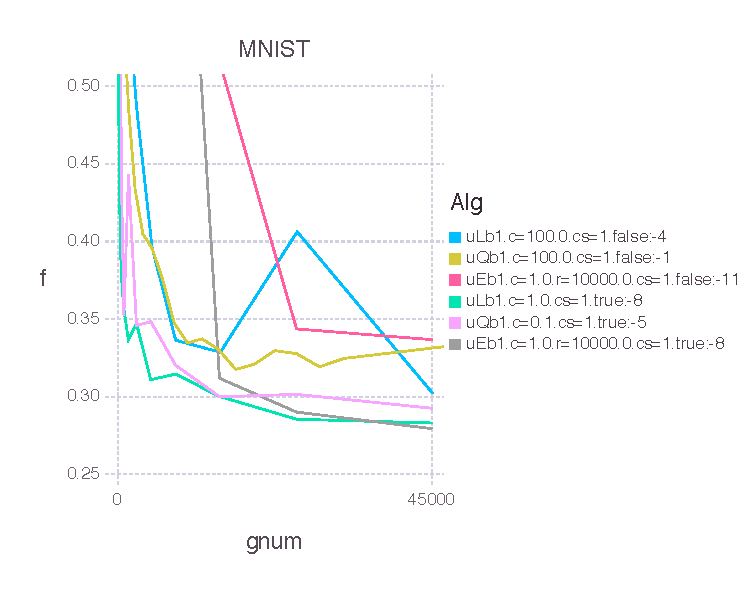
\includegraphics[width= 5in]{Figures/MNISTBLtruefInitialHeuristics.pdf}
   
   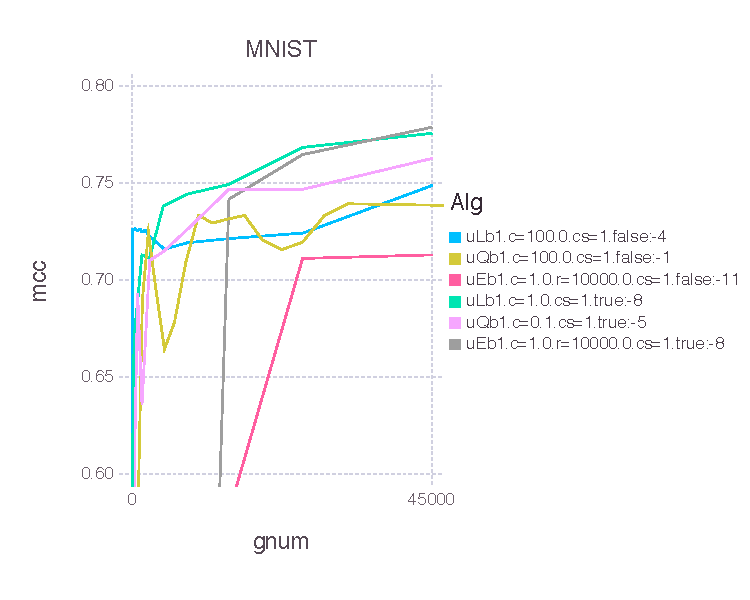
\includegraphics[width= 5in]{Figures/MNISTBLtruemccInitialHeuristics.pdf}
   
   \newpage
  
   \subsubsection{SG Comparison}
   
   Stepsizes were optimized to give best possible Testing function at the final iteration.

   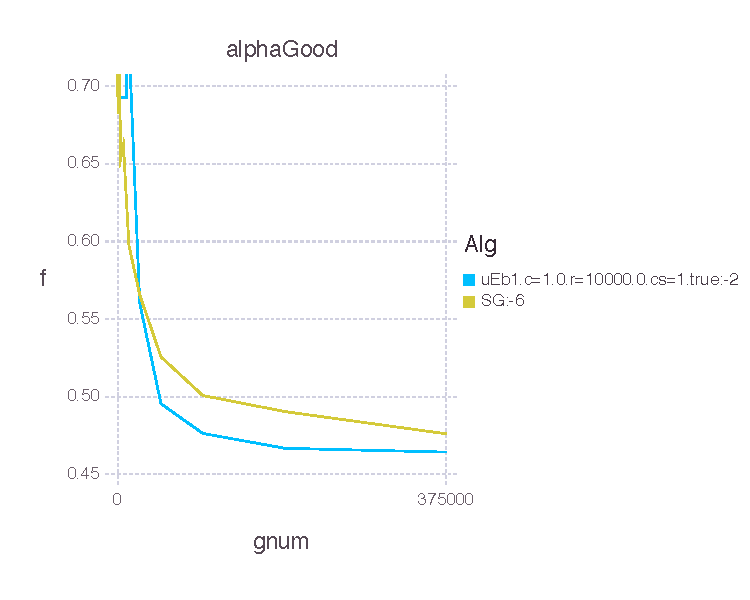
\includegraphics[width= 5in]{Figures/alphaGoodBLtruefWithSGglobal.pdf}
  
   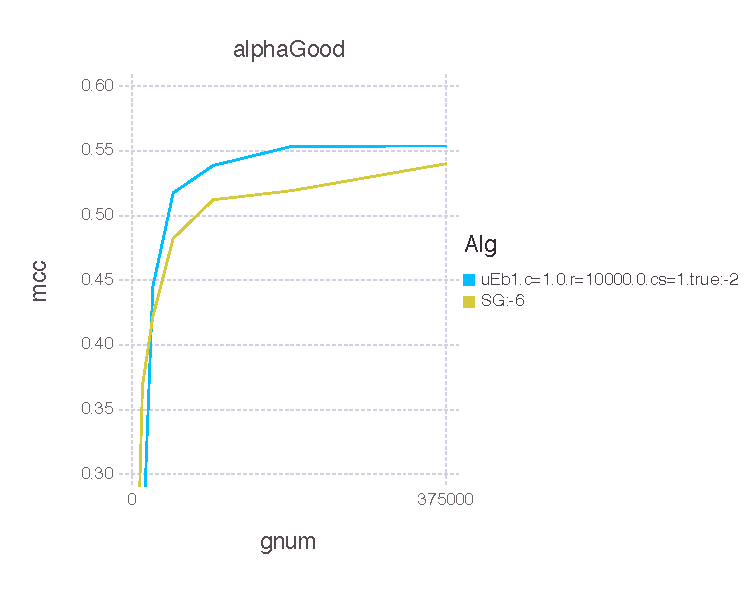
\includegraphics[width= 5in]{Figures/alphaGoodBLtruemccWithSGglobal.pdf}
   
   Stepsizes were optimized to give best possible Testing function value within the gradient evaluation limit.
   

   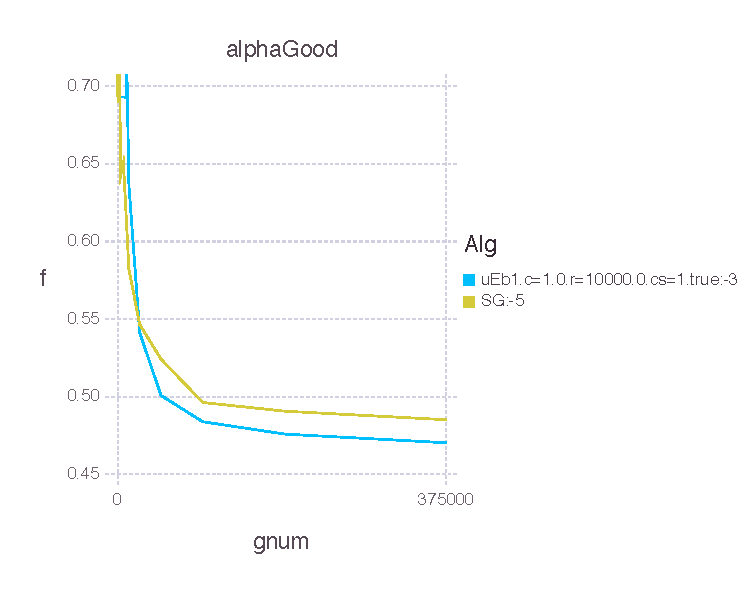
\includegraphics[width= 5in]{Figures/alphaGoodBLtruefWithSGoverTen.pdf}
  
   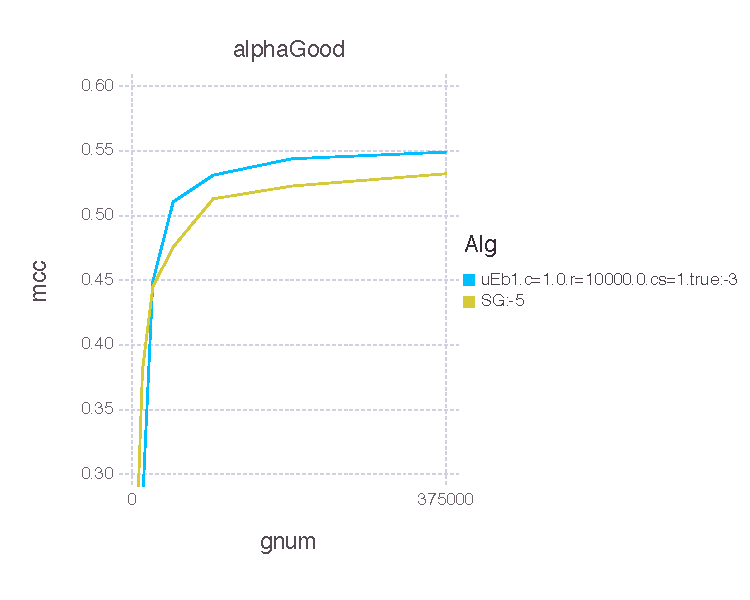
\includegraphics[width= 5in]{Figures/alphaGoodBLtruemccWithSGoverTen.pdf}
   
   
   \newpage
   
   \subsubsection{DSS Comparison}

   In this section, we show the difference between using the DSS method, and the EGR method with the same exponential growth rate.
   
   \newpage 
   
   \subsubsection{Performance Comparison}
   
   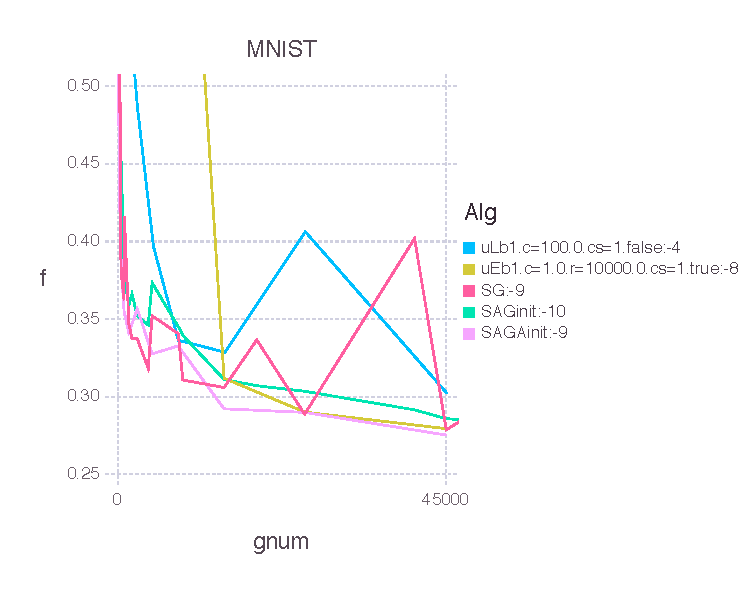
\includegraphics[width= 5in]{Figures/MNISTBLtruefOverall.pdf}
   
   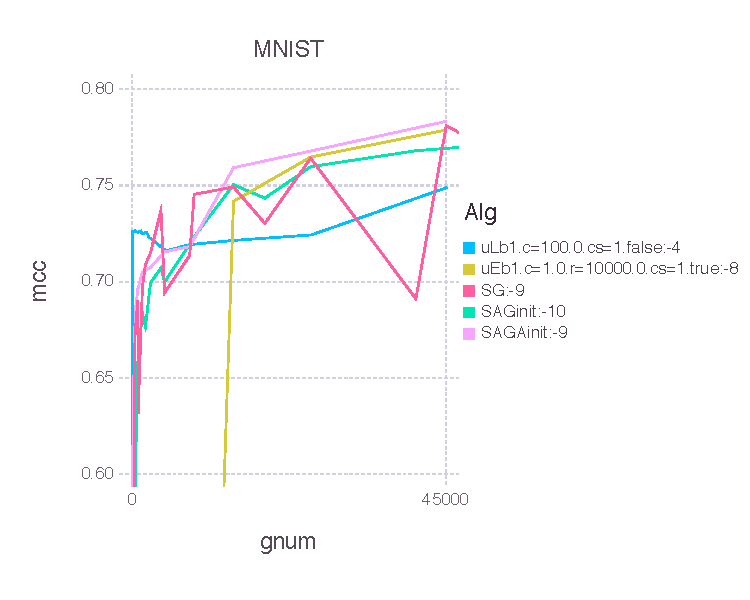
\includegraphics[width= 5in]{Figures/MNISTBLtruemccOverall.pdf}
   
   
   
\section{Final Remarks} \label{finalr}

\newpage \small 
\bibliographystyle{plain}

\bibliography{../References/references}


\end{document}

%%%%%%%%%%%%%%%%%%%%%%%%%%%%%%%%%
The suggested outline for the paper:
\begin{itemize}
	\item Define EGR
	\item Experiments
	\item Theory: 
	      \begin{itemize}
	\item EGR proof - only s (Figen's new proof)
	\item EGR-S proof - only s (My extension of SAGA proof)
	\item Work on extending to infinite case
	      \end{itemize}
		  \item Chunking
		  \begin{itemize}
		  	\item Batch-SAGA
		  	\item SAGA-SVRG continuum
		  	\item Representatives
		  \end{itemize}
\end{itemize}

Main question to figure out: 
\begin{itemize}
	\item Do our proof apply to a chunking technique?
	\item How to apply chunking to an unbounded problem? Maybe by growing chunks?
\end{itemize}

Questions about numerical experiments:
\begin{itemize}
	\item How does the training error look? Do we really need to plot training error?
	\item Variance evolution. Does it follow intuition?
	\item The three types of experiments: Are any of them more important/interesting than others? Other suggestions?
	      \begin{itemize}
	      	\item Multiple passes (5), methods that depend on $m$
	      	\item One pass, methods that do not use $m$
	      	\item Chunking?
	      	\item Other?
	      \end{itemize}
	\item Variety of test problems. What to note/compare in the experiments?
	\begin{itemize}
		\item Condition number
		\item Variance of gradients (or step directions)
		\item Sparse/dense
		\item Multiclass?
		\item Other loss functions?
		\item Regression vs classification?
		\item Diagonal dominance?
	\end{itemize}
\end{itemize}




\section{Introduction}






The minimizer of $F_m$ is $\theta^*_m$, and the corresponding objective value is $F^*_m$.  The relationship between these minima is well understood.

First, we have \cite[Proposition 10]{Kim:2015aa}  that 
$
         \mathbb{E} [F^*_m] \leq \mathbb{E} [F^*_{m+1}] \leq F^* ,
$
for any $m$, and under mild assumptions,
\[
         \mathbb{E} [ F^*_m ]-F^* = o(m^{-1/2}).
 \]
Furthermore, when a quadratic grown condition is satisfied we have that the minimizers satisfy,
\[ 
        \| \theta^*_m-\theta^*\| = O_p(m^{-1/2});
 \]
see \cite[Theorem 12]{Kim:2015aa}. Another result is cited in papers such as \cite{Frostig:2014aa} that state that under certain conditions on the distribution of $f^i$, we have 
\begin{equation}  \label{inc}
	\lim_{m \rightarrow \infty} \frac{\mathbb{E} \left[ F(\theta^*_m) - F*  \right] }{\sigma^2/m} = 1
\end{equation}
This means that we cannot hope to achieve better convergence rate than $O(1/m)$.

In Bottou-Bousquet\cite{bottou-bousquet-2008b}, it is stated that 
\begin{equation}
	\mathbb{E} \left[ \sup_{\theta} | F(\theta) - F_m(\theta) | \right] \leq c \sqrt{\frac{n}{m}}
\end{equation}
where the expectation is taken with respect to the random choice of the training set. 
\textcolor{blue}{JN: Stefan, compare these results carefully with those given in Bottou-Bousquet.}





%%%%%%%%%%%%%%
\section{The EGR Algorithm}


As already mentioned, the algorithm proposed in this paper is of the form \eqref{iteration}. At the $k$th iteration it adds some (say, $u_k$) new sample gradients to the running average, and at the same time, updates some (say, $s_k$) of the gradients previously stored. Thus, the total number of  gradients in the average, which we denote by $t_k$, increases. 

Specifically, the definition of $g^k$ in \eqref{iteration} is
\begin{align}  \label{gk}
	g^k = & \frac{1}{s_k+u_k} \left(  \sum_{j \in S_k} \left[  \nabla f_j(\phi_j^{k}) -  \nabla f_j(\phi^{k-1}_j) + \frac{1}{I_{k}} \sum_{i = 1}^{I_{k} }  \nabla f^i (\phi_i^{k-1})  \right] + \sum_{j \in U_k}  \nabla f_j(\phi_j^{k})\right). 
\end{align}
As we discuss below, this expression can be viewed as a variance reduced average of sampled gradients. Note the similarity with the SAGA iteration \eqref{saga}. The main changes are that the the second sum is over $t_k$ rather than $m$, that the first sum accounts for the fact that $S_k$ gradients in storage are updated, and the last sum represents the addition of $U_k$ gradients evaluated at the current iterate. A pseudocode is given in Algorithm~1

%%%% restart here
Concerning the sequence $\{ s_k \}$ that determines the number of points  revisited at each iteration, the variance reduction methods in \cite{many} use $s_k = 1$. In our algorithm, the value of $s_k$ can be larger in the light of the increasing size $t_k$ of the memory. Two natural choices are again $s_k = O(k)$ or $s_k= O(a^k)$.

Other choices of $u_k$ and $s_k$ are possible and give rise to some well known algorithms as illustrated in Table~\ref{tab1}. \textcolor{blue}{Maybe move this table to section 3?}
\bigskip
\begin{center} \label{tab1}
	\begin{tabular}  
		{ |c||c|c|c|c|c| } 
		\hline Algorithm & $u_k$ & $t_k$ & $\frac{u_k}{t_k}$ &$s_k$ for $k>0$ & $\frac{s_k}{I_k}$  \\
		\hline \hline \texttt{Only-add} & * & * & * & $0$ & $0$  \\
		\hline \texttt{Only-update}  &$ 
		\begin{array}{ll}
			m & \mbox{ if $k=0$} \\
			0 & \mbox{ if $k>0$} 
		\end{array}
		$& $m$ & $0$& * & * \\
		\hline \texttt{EGR-lin}  &$c$& $kc$ & $\frac{1}{k}$ &$c$ &$\frac{1}{k}$  \\
		\hline \texttt{EGR-quad}  &$c(k+1)$& $\frac{ck(k+1)}{2}$ & $\frac{2}{k}$ &$ck$ &$\frac{2}{k+1}$  \\
		\hline \texttt{EGR-exp}  &$ 
		\begin{array}{ll}
			c(r-1) & \mbox{ if $k=0$} \\
			c\left(\frac{r}{r-1}\right)^{k-1} & \mbox{ if $k>0$} 
		\end{array}
		$& $cr \left(\frac{r}{r-1}\right)^{k-2}$ & $\frac{1}{r-1}$&$c\left(\frac{r}{r-1}\right)^{k-1} $ &$\frac{1}{r-1}$\\
		\hline
	\end{tabular}
\end{center}
\bigskip

For simplicity, we did not include floor functions in the specifications of $s_k, u_k, I_k$, which are all integers. Some obvious adjustments must also be made to deal with special cases; for example for finite datasets of size $m$, the scalar $u_k$ must become $0$ once the whole training set has been exhausted. 



Two drawbacks are: this method is biased towards the samples included in $I$ early on. In addition, the required memory can approach $m$, and become unmanageable. This method is in itself a strategy to fill up the gradient memory from zero.




\subsection{Motivation: Variance Reduction}
To motivate the formula \eqref{gk}, we follow the argument given in  \cite{NIPS2014_5258} based on the control variate method of variance reduction.  Let $X$ and $Y$ be scalar random variables that are correlated. When the goal is to estimate $\mathbb{E} [X]$, an unbiased estimator of this quantity is
\[ Z_\beta = X - \beta ( Y - \mathbb{E}Y), \]
where $\beta \in \mathbb{R}$ is a control parameter parameter.
The variance is given by
\[ Var( Z_\beta) = Var(X) + \beta^2 Var(Y) -2 \beta Cov(X,Y). \]
When $X$ and $Y$ are correlated, the variance of the estimator is smaller than of $Var(X)$.

Choosing $X$ to be components of the sample gradient randomly chosen from the previously seen points, and $Y$ to be components of a previously computed gradient at that sample point, an unbiased estimate of the true gradient, with a (hopefully) reduced variance is
\[  \nabla f_j(\phi_j^{k}) - \beta_k \left( \nabla f_j(\phi^{k-1}_j) - \frac{1}{I_{k}} \sum_{i = 1}^{I_{k} }  \nabla f_i (\phi_i^{k-1}) \right). \]
When multiple such samples are considered, along with new sample gradients from unseen points, we can define an unbiased step of the form 
\begin{align*}
	g^k = & \frac{1}{s_k+u_k} \left(  \sum_{j \in S_k} \left[  \nabla f_j(\phi_j^{k}) - \beta_k \left(  \nabla f_j(\phi^{k-1}_j) - \frac{1}{I_{k}} \sum_{i = 1}^{I_{k} }  \nabla f_i (\phi_i^{k-1}) \right) \right] + \sum_{j \in U_k}  \nabla f_j(\phi_j^{k})\right). 
\end{align*}
Algorithm~1 employs to $\beta=1$. When $\beta_k=0$, the variance of the samples seen so far is not reduced. In general, the parameter $\beta_k$ can be tuned to the application.  A decreasing (increasing) sequence can be beneficial, because the variance reduction is more (less) important towards the end of the algorithm progress. 

\subsection{Related Methods}


The strategy of using an average gradient accumulated over all previous iterations occurs also in the \emph{Dual Averaging} method by Nesterov \cite{Nesterov:09}. That algorithm has the form
\[ \theta^{k+1} = -\frac{\sum_{i=1}^{k}g^i}{\beta^k}, \]
where each $g^i$ is a previously computed sample gradient, and $\beta^k$ is a  predefined sequence. Nesterov proves convergence results on the average iterate $\bar{\theta}^k = \frac{1}{k} \sum_{i=1}^{k} \theta^i$.

A natural question arises, why not use the average of the previously see gradients as a simple iterative step direction, of the form
\[ \theta^{k+1} = \theta^k- \alpha^k \frac{1}{k}\sum_{i=1}^{k}g^i . \]
The iteration above has not been analyzed, and it has never been used in practice because of poor performance. The past gradient average is a biased estimate of the true gradient, and certainly does not carry any second-order information.


%
%A similar method, SAG \cite{roux2012stochastic} has been proposed recently, and it has been effective on objectives of the form \eqref{saa}.
%\[ \theta^{k+1} = \theta^k- \alpha^k (\frac{1}{|I|} (  \nabla f_j(\theta^k) -  \nabla f_j(\phi_j^k)) + \frac{1}{|I|} \sum_{z_i \in I} \nabla f_i(\phi_i^k) ) \]
%. The step direction is once again a biased estimate of the gradient of $F_I$



A related method is SVRG, where the update direction is computed, at each iteration, by
\[ \nabla f_j(\theta^k) -  \nabla f_j(\tilde{\theta}) + \frac{1}{n}\sum_{i=1}^{n}  \nabla f_i (\tilde{\theta})\]

A method that is similar to ours is the Streaming SVRG method by 
SAGA assumes that initial sample gradients are known at $\theta^0$. Instead of using a full pass over the data, a heuristic is used to introduce data-points one-by-one. EGR does not rely on having a heuristic to jump-start the algorithm.

Another group of methods has iterations of the form
\begin{equation}
	\theta^k = \bar{\phi}^{k} - \alpha \frac{1}{m} \sum_{i=1}^{m} f'_i(\phi_i^k)
\end{equation}
where $\bar{\phi}^{k}$ is the current average of the historic points at which these sample gradients were evaluated. FINITO and MISO both follow this framework. They work on directly minimizing the average of the quadratic models corresponding to the individual samples. 
\begin{equation}
	\min \frac{1}{m} \sum_{i=1}^{m} \left[ f_i(\phi_i^k) + \langle \nabla f_i(\phi_i^k),y- \phi_i^k  \rangle + \alpha \|y-\phi_i^k  \|^2 \right]
\end{equation}
The proven convergence rate when $m \geq 2 \frac{L}{\mu}$, with a carefully chosen constant stepsize is 
\begin{equation}
	\mathbb{E} [F(\bar{\phi}^{k}) ] - F(\theta^*) \leq c \left( 1- \frac{1}{2m }\right)^k 
\end{equation}

The control variate idea is not new. "Variance Reduction for
Stochastic Gradient Optimization" paper by \cite{wang2013variance}.



\section{Parameter Discussion and Special Cases}

The algorithm presented requires three parameter sequences, but, as we demonstrate in the theory and the numerical results section, there are a few natural choices that have excellent properties. We suggest a parameter-free version that works well on all test problems encountered. 


\subsection{Choosing $\{s_k\}$ and $\{u_k\}$}

The algorithm specification requires that $s_0=0$, and $u_0>0$. $I_1 = u_0$, $I_2= u_0+u_1$, and in general $I_k = \sum_{i=0}^{k-1} u_i$ for $k>0$.

And additional necessary property is that $s_k \leq I_k$ for all $k$. 

In the following table we summarize all the choices of the growth sequences we considered, and provide additional details in the following subsections. 

Remember that these are not precisely implementable: A floor function is always used in the computation of $s_k$ and $u_k$.

In addition, for finite datasets of size $m$, $u_k$ must become $0$ once the whole training set has been exhausted. 

Some attempts to heuristically find the best growth rates are documented in Appendix~\ref{appendix:heuristics}.

\subsubsection{\texttt{Only-add}}

Many methods fall into this category, such as the incremental gradient method with a randomized order, stochastic gradient, and the DSS method \cite{dss}. These methods have been exhaustively explored, and are nevertheless very competitive in practice. The results are about how fast the true objective evaluated at the current iterate approaches $F^*$.

Bertsekas and Nedic\cite{nedic2001convergence} show that for an incremental gradient method with a randomized order, for a constant stepsize $\alpha$, we have 
\begin{equation}
	\inf_{k \geq 0} F_m(\theta^k) \leq F_m^* + 2.5 \alpha m c^2
\end{equation}
where $\| \nabla f_i(\theta) \| \leq c$, for any $i$ and $\theta$. 

They state that such a method with decreasing stepsizes converges (because it is possible to view the incremental gradient method with a randomized selection of the component function as a stochastic gradient method).

Finally, for a randomized method with a strong convexity assumption on $F$, we have that for $\alpha_k = \frac{R}{k+1}$,  $\mathbb{E} \|\theta^{k+1} - \theta^* \|^2  $ is of order $O(\frac{1}{k})$.


\subsubsection{\texttt{Only-update}}

Two major methods fall into this category: the classic gradient descent algorithm, and SAGA. These algorithms work on a static batch of size $m$. Most of the proven results are about the quantity $F^*_m$, but some also estimate $\|  \theta^K_m - \theta^*\|$.

This is the standard gradient descent method, applied to the function $F_m(x)$. The following standard results from convex optimization are known 
\begin{thm}
	\label{thm:gd1}
	For $\alpha_k = \frac{1}{L}$, and $F_{m} \in \mathcal{F}_L^{1,1} (R^n)$ 
	\begin{equation}
		F_m(\theta^{k}) - F_m^* \leq \frac{2 \|\theta_0-\theta^* \|^2}{k+4} 
	\end{equation}
\end{thm}
\begin{thm}
	\label{thm:gd2}
	For $\alpha_k = \frac{2}{\mu+L}$, and $F_{m} \in \mathcal{S}_{\mu,L}^{1,1} (R^n)$ 
	\begin{equation}
		F_m(\theta^{k}) - F_m^* \leq \frac{L}{2} \left( \frac{L/\mu-1}{L/\mu+1} \right)^{2k} \|\theta_0-\theta^* \|^2 
	\end{equation}
\end{thm}
\begin{thm}
	\label{thm:gd3}
	For $\alpha_k = \alpha  \in (0,2/L)$, and $F_{m} \in \mathcal{S}_{\mu,L}^{1,1} (R^n)$ 
	\begin{align*}
		\| \theta^{k+1} - \theta^* \|  &\leq \max \{ |1 -\alpha \mu|, |1 - \alpha L| \}\| \theta^{k} - \theta^* \| \\
		& \leq {\left(\max \{ |1 -\alpha \mu|, |1 - \alpha L| \}\right)}^{k}\| \theta^{0} - \theta^* \| \\
	\end{align*}
\end{thm}
\begin{thm}
	\label{thm:gd4}
	For $\alpha_k = \frac{2}{\mu+L}$, and $F_{m} \in \mathcal{S}_{\mu,L}^{1,1} (R^n)$ 
	\begin{align*}
		\| \theta^{k+1} - \theta^* \|  &\leq \frac{L/\mu-1}{L/\mu+1}\| \theta^{k} - \theta^* \| \\
		& \leq {\left(\frac{L/\mu-1}{L/\mu+1}\right)}^{k}\| \theta^{0} - \theta^* \| \\
	\end{align*}
\end{thm}

Don't forget that 
\begin{align*}
	\frac{L/\mu-1}{L/\mu+1} & = 1 - (1 - \frac{L/\mu-1}{L/\mu+1}) \\
	 						& = 1 - (\frac{L/\mu+1}{L/\mu+1} - \frac{L/\mu-1}{L/\mu+1}) \\
	 						& = 1 - \frac{2}{L/\mu+1}\\
\end{align*}

Recent results by Royset and Szechtman \cite{royset2013optimal}, state that for such an algorithm, if $c = n \times k$,
\[ \left( \frac{c}{a \log c}\right)^{1/2} (F_I(\theta^{k}) -F^*) = O(1) \]

For SAGA,the convergence results from \cite{NIPS2014_5258} apply directly. A linear convergence rate is established in the case of strong convexity of $f$: 
\begin{equation}
	\mathbb{E}{\| x^k - x^*_c\|}^2 \leq {\left( 1- \frac{\mu}{2 (\mu n +L)}\right)}^k \left[ {\| x^0 - x^*_c\|}^2 + \frac{n}{\mu n +L} F_c(x^0) - \langle  \nabla f_c(x^*_c), x^0 - x^*_c\rangle - F_c(x^*_c) \right] 
\end{equation}

\subsubsection{\texttt{egr-lin}}

\subsubsection{\texttt{egr-quad}}

\subsubsection{\texttt{egr-exp}}

The motivation for this growth rate is the desire to grow both the $\{I_k\}$ sequence by a fixed fraction at every iteration. This strategy starts with a large initial batch of size $c(r-1)$ for $u_0$, and then computes a constant fraction of $I_k$ and resamples that amount, thus growing at an exponential rate. 

We found, experimentally, that a value for $c=1$ and for $r = \frac{K}{400}$ where $K$ is the total number of iterations provides an overall well performing growth sequence. 

\subsection{Choosing $\{\alpha_k\}$}

In the spirit of methods that have continually improving gradient estimates as the algorithm progresses, we suggest using a fixed step size $\{\alpha_k\} = \alpha$. 

\section{Theory}

\subsection{To Prove}

The EGR algorithms have two types of convergence. The convergence to the true optimal objective value $F^*$ can at best be $O(\frac{1}{n})$. The two types of results we can show for $F^*$ are

\begin{thm}
	\label{thm:our}
	For some assumptions, 
	\begin{equation}
		F(\theta^{k}) - F^*
	\end{equation}
	is $O(\frac{1}{k})$ for some good constant, where $k$ is the total number of gradient evaluations to reach $\theta^{k}$
\end{thm}

\begin{thm}
	\label{thm:our}
	For some assumptions, 
	\begin{equation}
		F(\theta^{k}) - F^*
	\end{equation}
	is decreasing exponentially, where $k$ is the outer iteration count to reach $\theta^{k}$. These assumptions will probably require exponential growth in $s_k$ and $u_k$
\end{thm}

Furthermore, we can prove results for the finite sample case, such as
\begin{thm}
	\label{thm:our}
	For some assumptions, 
	\begin{equation}
		F(\theta^{k}) - F^*_m
	\end{equation}
	is decreasing exponentially, where $k$ is the total number of gradient evaluations to reach $\theta^{k}$ and $u_k$
\end{thm}

And, maybe a REGRET BOUND result!
\begin{thm}
	Let the regret function be 
	\begin{equation}
		R(T) = \sum_{t=1}^{T} \left[ f_t(\theta^t) - f_t(\theta^*)\right]
	\end{equation}
\end{thm}

\subsection{Finite incremental gradient proof!}


\subsection{Finite GD-like proof}


\subsection{DSS-like proof}

Let 
\begin{equation}
	\theta_{k+1} = \theta_k - \frac{1}{L} g^k 
\end{equation}

By Taylor's theorem, for any $g^k$, we have that 
\begin{equation}
	F(\theta_{k+1}) \leq F(\theta_k) - \frac{1}{L} \nabla F (\theta_k)^T g^k + \frac{1}{2L} \|g^k\|^2 
\end{equation}

Assume $\theta_k$ is constant. Then, the only random quantity in the expression above is $g^k$.

Taking expectations, and using $\mathbb{E} [g^k] = \nabla F(\theta_k)$, we have 
\begin{align*}
	\mathbb{E} [ F(\theta_{k+1}) ] & \leq F(\theta_k) - \frac{1}{L} \nabla F (\theta_k)^T\mathbb{E} [g^k] + \frac{1}{2L} \mathbb{E}[ \| g^k \|^2] \\
	& =F(\theta_k) - \frac{1}{L} \|\nabla F(\theta_k)\|^2 + \frac{1}{2L} (\|\nabla F(\theta_k)\|^2 + \sum_{i=1}^n \Var ( g^k_i) )
\end{align*}

Using $\nabla F(\theta)^T \nabla F(\theta) \geq \lambda \ (F(\theta ) - F^*)$ we have that
\begin{align*}
	\mathbb{E} [ F(\theta_{k+1}) ]  - F^* & \leq F(\theta_k) - \frac{1}{2L} \lambda \ (F(\theta_k) - F^*)   - F^*+ \frac{1}{2L}\Var (\| g^k\|) \\
                                          & =( 1-\frac{\lambda}{2L})  \ (F(\theta_k) - F^*)+ \frac{1}{2L}\sum_{i=1}^n \Var ( g^k_i)
\end{align*}

	
	\subsubsection{linear}
	
Assume 
\begin{equation}
	\mathbb{E} [ F(\theta_{k}) ]  - F^* \leq C p^k 
\end{equation}
for some $k$. Then, 
	\begin{align*}
		\mathbb{E} [ F(\theta_{k+1}) ]  - F^* & \leq ( 1-\frac{\lambda}{2L})   (F(\theta_k) - F^*)+ \frac{1}{2L}\sum_{i=1}^n \Var ( g^k_i) \\
											  & \leq ( 1-\frac{\lambda}{2L})   C p^k+ \frac{1}{2L}\sum_{i=1}^n \Var ( g^k_i)\\
											  & = C p^k ( 1-\frac{\lambda}{2L} + \frac{1}{2LC p^k }\sum_{i=1}^n \Var ( g^k_i)) \\
											  & \leq C p^{k+1}  
	\end{align*}
	with the condition that 
	\begin{equation}
		1-\frac{\lambda}{2L} + \frac{1}{2LC p^k }\sum_{i=1}^n \Var ( g^k_i) \leq p
	\end{equation}
	To guarantee this, we need 
	\begin{align*}
		 \sum_{i=1}^n \Var ( g^k_i) &\leq \left( p -1 +\frac{\lambda}{2L} \right) 2LC p^k  \\
		 &= 2LC p^{k+1} -2LC p^k +C p^k\lambda \\
		 &= C p^k \left( 2L p -2L +\lambda \right)  \\
	\end{align*}

To achieve a linear decrease in the objective value, $p$ must be strictly less than 1, and therefore the variance must go to zero. $p$ must also satisfy
\begin{equation}
	p \geq 1 -\frac{\lambda}{2L} 
\end{equation}
	
	So there are two ways of satisfying this. Either variance goes to zero because of an increasing batch size, or because of some other mechanism, such as our iterates being close enough together that the variance reduction technique gives a variance that decreases fast enough. This is indeed the case for the SAGA algorithm. 

For the SAGA algorithm, plug in 
	\begin{align*}
		 \sum_{i=1}^n \Var(X_i) + \Var(Y_i) -2 Cov(X_i,Y_i) &\leq \left( p -1 +\frac{\lambda}{2L} \right) 2LC p^k  \\
		 &= 2LC p^{k+1} -2LC p^k +C p^k\lambda \\
		 &= C p^k \left( 2L p -2L +\lambda \right)  \\
	\end{align*}
	
	Furthermore, if we define $D_i$ to be a random variable (dependent on $X$ and $Y$) that satisfies  $Y_i = X_i + D_i$, we arrive at 
	\begin{align*}
		 \sum_{i=1}^n \Var(D_i) &\leq \left( p -1 +\frac{\lambda}{2L} \right) 2LC p^k  \\
		 &= 2LC p^{k+1} -2LC p^k +C p^k\lambda \\
		 &= C p^k \left( 2L p -2L +\lambda \right)  \\
	\end{align*}
	
	
	\subsubsection{sublinear}
	Let's go the other route, to get sublinear convergence!
	
	Assume 
	\begin{equation}
		\mathbb{E} [ F(\theta_{k}) ]  - F^* \leq \frac{C}{k} 
	\end{equation}
	
	\begin{align*}
		\mathbb{E} [ F(\theta_{k+1}) ]  - F^* & \leq ( 1-\frac{\lambda}{2L})   (F(\theta_k) - F^*)+ \frac{1}{2L}\sum_{i=1}^n \Var ( g^k_i) \\
											  & \leq ( 1-\frac{\lambda}{2L})   \frac{C}{k}+ \frac{1}{2L}\sum_{i=1}^n \Var ( g^k_i)\\
											  & \leq  \frac{C}{k+1} 
	\end{align*}
	
	For this to be true, must have that 
	\begin{align*}
 ( 1-\frac{\lambda}{2L})   \frac{C}{k}+ \frac{1}{2L}\sum_{i=1}^n \Var ( g^k_i) \leq  \frac{C}{k+1} 
	\end{align*}
	Solving for the variance term, we get 
	\begin{align*}
	\sum_{i=1}^n \Var ( g^k_i) & \leq  \frac{2CL}{k+1}  -( 1-\frac{\lambda}{2L})   \frac{2CL}{k} \\
	& =  \frac{2CL}{k+1}  - \frac{2CL}{k} +  \frac{\lambda}{2L}   \frac{2CL}{k} \\
	& =  \frac{2CLk}{k(k+1)}  - \frac{2CL(k+1)}{k(k+1)} +  \frac{\lambda (k+1)}{2L}   \frac{2CL}{k(k+1)} \\
	& =  \frac{2CLk}{k(k+1)}  - \frac{2CL(k+1)}{k(k+1)} +   \frac{C\lambda (k+1)}{k(k+1)}\\
	& =   \frac{C\lambda (k+1) - 2CL}{k(k+1)} \\
	& =  C \left( \frac{\lambda}{k} - \frac{2L}{k(k+1)}\right) 
	\end{align*}

Here the variance still needs to go to zero!	
	
\subsection{TO DO}

put in the variance in Figen proof

\subsection{Quadratic Case}

 
\noindent 
Consider the quadratic finite sum minimization problem with $N$ data points, 
\[
 F(x) = \frac{1}{N}\sum_{i=1}^N f_i(x),
\]
and an extension of the SAG algorithm that updates each gradient component with probability $\eta$ at each iteration.  Let 
\[
 x_{k+1} = x_k -\alpha y_k
\]
and
\[
 y_k = \frac{1}{N}\sum_{i=1}^N \nabla f_i(x_{k(i)}) 
\]
where
\[
 \begin{cases}
  k(i) = k  & \mbox{ with probability }\eta,\\
  k(i) = [k-1](i) & \mbox{ with probability }1-\eta.
 \end{cases}
\]

It is necessary to define the initial $k$'s, for example by $[0](i)=0$.

\bigskip

\noindent
Define error terms 
\[
 e_k^i = \nabla f_i(x_{k(i)})-\nabla f_i(x_k) \qquad \mbox{and} \qquad e_k=\frac{1}{N}\sum_{i=1}^N e_k^i
\]
so that we can state 
\[
 y_k = \frac{1}{N}\sum_{i=1}^N (\nabla f_i(x_k)+e_k^i) = \nabla f(x_k) + e_k.
\]
Furthermore, 
\begin{align*}
 e_k^i = \nabla f_i(x_{k(i)})-\nabla f_i(x_{k-1})+\nabla f_i(x_{k-1})-\nabla f_i(x_k).
\end{align*}
	
Note that given $e_{k-1}$ and $x_{k-1}$, we have the conditional expectation 
\[
 E[e_k^i] = (1-\eta)(e_{k-1}^i + \nabla f_i(x_{k-1}) -\nabla f_i(x_k).
\]

\bigskip
\noindent
Finally, let us define two average Hessian matrices, $H_k$ and $\bar H_k$, for each $k$, such that
\[
 \nabla f(x_k) = \nabla f(x_{k-1})+H_k(x_k-x_{k-1}),
\]
\[
 \nabla f(x_k) = \bar H_k(x_k-x_\ast),
\]
and assume that 
\[
  \mu I \preceq H_k \preceq L I , \quad \mbox{and} \quad \mu I \preceq \bar H_k \preceq L I,\quad \mbox{for all }k
\]
are satisfied for some $\mu>0$ and $L>1$.

\bigskip

\noindent 
Now, we will write two relations on the change of $e_k$ and on the change of $x_k-x_\ast$, respectively, and then merge the two.
 \begin{align*}
  E[e_k] &= (1-\eta)(e_{k-1} + \nabla f_{k-1} - \nabla f_k)\\
  &= (1-\eta)(e_{k-1} - H_k(x_k-x_{k-1}))\\
  &= (1-\eta)(e_{k-1} - H_k(-\alpha y_{k-1}))\\
  &= (1-\eta)\left(e_{k-1} + \alpha H_k (\nabla f_{k-1}+e_{k-1})\right)\\
  &= (1-\eta)\left((I+\alpha H_k)e_{k-1} + \alpha H_k\nabla f_{k-1}\right)\\ 
  &= (1-\eta)(I+\alpha H_k)e_{k-1} + (1-\eta)\alpha H_k\bar H_{k-1}(x_{k-1}-x_\ast),
 \end{align*}
and
 \begin{align*}
  x_k-x_\ast &= x_{k-1}-x_\ast + (x_k-x_{k-1})\\
  &=x_{k-1}-x_\ast -\alpha y_{k-1}\\
  &=x_{k-1}-x_\ast -\alpha (\nabla f_{k-1} + e_{k-1})\\
  &=x_{k-1}-x_\ast -\alpha\bar H_{k-1}(x_{k-1}-x_\ast) -\alpha e_{k-1}\\
  &=(I-\alpha\bar H_{k-1})(x_{k-1}-x_\ast) -\alpha e_{k-1}.
 \end{align*}
 
\bigskip

\noindent  
So, merging the two equations yields,
\[
 \begin{pmatrix} \displaystyle\frac{1}{L}E[e_k] \\ x_k-x_\ast \end{pmatrix} 
= M_k
 \begin{pmatrix} \displaystyle\frac{1}{L}e_{k-1} \\ x_{k-1}-x_\ast \end{pmatrix}  \quad\mbox{for}\quad 
 M_k = \begin{pmatrix} (1-\eta)(I+\alpha H_k) & \displaystyle\frac{1}{L} (1-\eta)\alpha H_k\bar H_{k-1}\\  
                   -\alpha LI  & I-\alpha\bar H_{k-1} \end{pmatrix}.                   
\]

\bigskip
\noindent
We will consider choosing 
\[
 \alpha = \frac{\eta}{L}.
\]
With this choice of $\alpha$, we get
\[
 \|M_k^{11}\|= \|(1-\eta)(I+\frac{\eta}{L}H_k)\|\leq (1-\eta)(1+\eta) = 1-\eta^2 \leq 1,
\]
\[
 \|M_k^{12}\|= \|\frac{1}{L} (1-\eta)\frac{\eta}{L} H_k\bar H_{k-1}\|\leq \eta(1-\eta)\leq 1,
\]
\[
 \|M_k^{21}\|= \|-\frac{\eta}{L} LI \|\leq \eta \leq 1,
\]
\[
 \|M_k^{22}\|= \|I-\frac{\eta}{L}\bar H_{k-1} \|\leq 1-\eta\frac{\mu}{L} \leq 1.
\]


% \noindent
% Consider the following partitioning of the matrix $M_k$.
% \[
% T + E
% =\begin{pmatrix} (1-\sigma)(I+\alpha H_k) & (1-\sigma)\alpha H_k\bar H_{k-1}\\  
%                    0  & I-\alpha\bar H_{k-1} \end{pmatrix}              
% +\begin{pmatrix} 0 & 0 \\  
%                    -\alpha I  & 0 \end{pmatrix}                   
% \]
% Since $T$ is block triangular, it is eigenvalues are the eigenvalues of $T_{11}=(1-\sigma)(I+\alpha H_k)$ and $T_{22}=(I-\alpha\bar H_{k-1})$. (Let us denote these eigenvalues with $v$ and $w$, respectively).  Moreover, if $V$ and $W$ are the matrices containing the eigenvectors of $T_{11}$ and $T_{22}$, respectively, then the eigenvectors of $T$ are
% \[
%  R=\begin{pmatrix} V & K \\  
%                    0 & W \end{pmatrix},                   
% \]
% where the $ith$ column of $K$ is given as
% \[
%  K_i = -(T_{11}-w_iI)^{-1}T_{12}W_i.
% \]
% Note that $T_{11}$ and $T_{22}$ are symmetric; so, $V$ and $W$ are unitary matrices.  Also,
% \[
%  R^{-1}=\begin{pmatrix} V^{-1} & -V^{-1}KW^{-1} \\  
%                    0 & W^{-1} \end{pmatrix}.                   
% \]
% Then,
% \[
%  \kappa_1(R)=\|R\|_1\|R^{-1}\|_1\leq\max_i (\|K_i\|_1+1)^2
% \]
% The Bauer-Fike theorem implies that the maximum absolute gap between an eigenvalue $\lambda$ of $M_k$ and the eigenvalue of $A$ closest to $\lambda$ is 
% \[
%  \kappa_1(R)\|E\|_1 \leq \max_i (\|K_i\|_1+1)^2 \alpha.
% \]
% 
% 
% \bigskip\bigskip
% 
% 
% \paragraph{Goal:} $\lambda_{\max}(M_k)\leq \max\{1-\alpha\mu, (1-\sigma)(1+L\alpha)\}$ for $\alpha = \displaystyle\frac{\sigma}{L}$.
% 
% \noindent
% So, 
% \[
% 0<\lambda_{\max}(M_k)\leq \max\{1-\alpha\mu, (1-\sigma)(1+L\alpha)\}= \max\{1-\sigma\frac{\mu}{L}, 1-\sigma^2\}<1.
% \]


%\newpage

\bigskip\bigskip

\noindent
This result could be easily adapted to the growing sample case (as long as we provide that the gradient of each component function is updated with probability $\eta$) because there is no dependence on the sample size.


% \noindent 
% Note that there is no dependence on $N$ here.  To extend this result to the infinite sum case, we will consider the expectation wrt $z$ as well as the expectation wrt $\sigma$.  Also, we will no more assume that the memory size is fixed, we will denote the memory size at iteration $k$ as $|I_k|$, and will consider the iterations with $|I_k|>N$ for some $N$. 

 
\noindent 
Let us consider the following matrix
\[
 M_k = \begin{pmatrix} (1-\eta)(I+\alpha H_k) & \displaystyle\frac{1}{L} (1-\eta)\alpha H_k\bar H_{k-1}\\  
                   -\alpha LI  & I-\alpha\bar H_{k-1} \end{pmatrix}                  
\]
with $\alpha=\displaystyle\frac{\eta}{4L}$.

% \bigskip
% \noindent
% In our experiments on the minimization of the sum of random quadratics, we observed that this matrix always have all eigenvalues less than 1 (even if it has singular values slightly larger than 1!).  As expected, the maximum eigenvalue decreases as $\eta$ increases (which should indicate a higher convergence rate).  The following table illustrates the situation on instances with problem dimension($n$)=20, and component functions($N$)=100.  In all cases, the condition number is around $10^{-2}$, and $L$ is around $5\times 10^3$.
% \begin{center}
% \begin{tabular}{ccc}
%  \hline
%  $\eta$ & max(eigenvalue(M\_k)) & max(singular\_value(M\_k)) \\
%  \hline
%  0.01 & 0.9999 & 1.0001 \\
%  0.05 & 0.9998 & 1.0006 \\
%  0.1 & 0.9997 & 1.0013 \\
%  0.5 & 0.9983 & 1.0087 \\
%  \hline
% \end{tabular}
% \end{center}
%
% \bigskip

If we can generalize our numerical observation and prove that the spectral radius of this matrix is always less than 1, that would indicate 
\[
\prod_{t=1}^\infty M_t \rightarrow 0. 
\]
Since the random processes at each iteration are independent, this would provide $E[e_k, x_k-x_\ast]\rightarrow 0$ (did not yet think about the variance).


\bigskip

\paragraph{Bounding the spectral radius.}
To simplify $M_k$, let us for now set $\bar H_{k-1}=H_k=H$.  So, $M_k$ becomes
\[
M = \begin{pmatrix} (1-\eta)(I+\displaystyle\frac{\eta}{4L} H) & \displaystyle(1-\eta)\frac{\eta}{4L^2} HH\\ 
 \\
                   -\displaystyle\frac{\eta}{4}I  & I-\displaystyle\frac{\eta}{4L} H \end{pmatrix}.                  
\]
Let us first observe that 
\begin{align*}
\sum_i \lambda_i = trace(M) &= trace(M_{11})+trace(M_{22})\\
&=trace((1-\eta)(I+\frac{\eta}{4L} H))+trace(I-\frac{\eta}{4L} H)\\
&\geq n(1-\eta)(1+\frac{\eta\mu}{4L})+n(1-\frac{\eta}{4})>0,
\end{align*}
and
\begin{align*}
\prod_i \lambda_i = \det(M) &= \det\left((1-\eta)(I+\alpha H)(I-\alpha H) + (1-\eta)\alpha^2 HH\right)\\
&=\det\left((1-\eta)I\right) = (1-\eta)^n<1.\\
\end{align*}

\bigskip
\paragraph{Lemma 1.} The largest eigenvalue of $M$ is less than 1.  

\bigskip

\noindent
\textit{Proof.} Each eigenvalue $\lambda$ of $M$ by definition satisfies $\det(M-\lambda I)=0$.  Therefore,
\[
 \det \begin{pmatrix} (1-\eta)(I+\displaystyle\frac{\eta}{4L} H)-\lambda I & \displaystyle(1-\eta)\frac{\eta}{4L^2} HH\\ 
 \\
                   -\displaystyle\frac{\eta}{4}I  & I-\displaystyle\frac{\eta}{4L} H -\lambda I  \end{pmatrix}=0
\]
Since blocks $M_{21}$ and $M_{22}$ commute we have
\[
 \det\left((1-\eta)(I+\frac{\eta}{4L} H)-\lambda I)(I-\frac{\eta}{4L} H -\lambda I) + (1-\eta)\frac{\eta^2}{4^2L^2} HH \right)=0.
\]

With some algebra, this statement simplifies to 
\[
 \det\left((1-\lambda)(1-\lambda-\eta)I + \eta^2 \frac{\lambda}{4L}H \right)=0.
\]

Then, $-(1-\lambda)(1-\lambda-\eta)$ is an eigenvalue of the matrix $\eta^2 \displaystyle\frac{\lambda}{4L}H$; so,
\begin{equation}
 -(1-\lambda)(1-\lambda-\eta) \in \left[\frac{\eta^2\lambda\mu}{4L},\frac{\eta^2\lambda}{4}\right]
 \label{eq:p}
\end{equation}
should hold.

The concave function $p(\lambda)= -(1-\lambda)(1-\lambda-\eta)$ has two roots at $\lambda=1$ and at $\lambda=1-\eta$.  Then, $p(\lambda)<0$ for $\lambda>1$ and for $\lambda<1-\eta$.  So, having $\lambda>1$ is inconsistent with \eqref{eq:p}.  

\bigskip

\paragraph{Lemma 2.}$M$ has no negative eigenvalues.  

\bigskip

\noindent
\textit{Proof.} Suppose that $\lambda<0$ is an eigenvalue of $M$.  Then, $p(\lambda)\geq \displaystyle\frac{\eta^2 \lambda}{4}$ by \eqref{eq:p}(since $\lambda<0$). That is,
\begin{align*}
 &-(1-\lambda)(1-\lambda-\eta) \geq \displaystyle\frac{\eta^2 \lambda}{4}\\
 \Rightarrow&-\lambda^2+(2-\eta-\displaystyle\frac{\eta^2}{4})\lambda+\eta-1\geq 0.  
\end{align*}
The smaller root of the polynomial on the left hand side is
\begin{align*}
 &-\frac{1}{2}\left(-(2-\eta-\displaystyle\frac{\eta^2}{4})+\sqrt{(2-\eta-\displaystyle\frac{\eta^2}{4})^2+4(1-\eta)}\right)\\
 &=1-\frac{\eta}{2}-\frac{\eta^2}{8}-\frac{1}{8}\sqrt{\eta^4+8\eta^3}>1-\eta\geq 0 \quad \mbox{for}\quad \eta\in(0,1]
\end{align*}
as $\ \displaystyle\frac{\eta}{2}+\frac{\eta^2}{8}+\frac{1}{8}\sqrt{\eta^4+8\eta^3}<\frac{\eta}{2}+\frac{\eta}{8}+\frac{3\eta}{8}=\eta$.
Therefore, $p(\lambda)\geq \displaystyle\frac{\eta^2 \lambda}{4}$ cannot be satisfied for $\lambda<0$.  

\bigskip

Thus, we can conclude that for all eigenvalues of $M$ we have $\lambda\in(1-\eta,1)$.  We will next investigate the $\lambda$ values that satisfy $p(\lambda)\leq \displaystyle\frac{\eta^2 \lambda}{4}$ and $p(\lambda)\geq \displaystyle\frac{\eta^2 \lambda\mu}{4L}$ to obtain a tighter bound for the spectral radius.  Even if we saw that $\lambda$ is strictly less than 1 provided that we have strong convexity ($\mu>0$), we wish to know how it depends on $\mu$, $L$, and $\eta$.

\bigskip

\paragraph{Theorem.} For all eigenvalues $\lambda$ of $M$
\[
 \lambda\in\left(1-\eta \ , \ 1-\frac{\eta}{2}-\frac{\eta^2}{2}\right)\cup\left(1-\frac{\eta}{2}+\frac{\eta^2}{4} \ , \ 1-\frac{\mu\eta^2}{4L}\right)
\]
holds.  So, the spectral radius of $M$ is less than $1-\displaystyle\frac{\mu\eta^2}{4L}$.


\bigskip

\noindent
\textit{Proof.} 
\begin{itemize}
 \item[I.] Consider $p(\lambda)\leq \displaystyle\frac{\eta^2 \lambda}{4}$. We have already derived the roots of the polynomial $p(\lambda)-\displaystyle\frac{\eta^2 \lambda}{4}$. Then, 
 for the smaller root $\lambda_{s1}$ we have $\lambda_{s1}<1-\displaystyle\frac{\eta}{2}-\displaystyle\frac{\eta^2}{2}$, and for the larger root $\lambda_{l1}$ we have $\lambda_{l1}>1-\displaystyle\frac{\eta}{2}+\displaystyle\frac{\eta^2}{4}$.  So, if $p(\lambda)-\displaystyle\frac{\eta^2 \lambda}{4}\leq 0$, then either $\lambda < 1-\displaystyle\frac{\eta}{2}-\displaystyle\frac{\eta^2}{2}$ or $\lambda > 1-\displaystyle\frac{\eta}{2}+\displaystyle\frac{\eta^2}{4}$ (but not vice versa).
 \item[II.] Consider $p(\lambda)\geq \displaystyle\frac{\eta^2 \lambda\mu}{4L}$.  The larger root of the polynomial $p(\lambda)-\displaystyle\frac{\eta^2 \lambda\mu}{4L}$ is
 \[
  \lambda_{l2} = 1-\frac{\eta}{2}-\frac{\mu\eta^2}{8L}+\frac{\eta}{2}\sqrt{1-\frac{\mu}{L}+\frac{\mu\eta}{2L}+\left(\frac{\mu\eta}{4L}\right)^2}<1-\frac{\mu\eta^2}{4L}
 \]
as 
 \[
  \sqrt{1-\frac{\mu}{L}+\frac{\mu\eta}{2L}+\left(\frac{\mu\eta}{4L}\right)^2} = \sqrt{\left(1-\frac{\mu\eta}{4L}\right)^2-(1-\eta)\frac{\mu}{L}}<1-\frac{\mu\eta}{4L}.
 \]
Using the same argument, we observe that for the smaller root we have $\lambda_{s2}>1-\eta$.  So, if $p(\lambda)- \displaystyle\frac{\eta^2 \lambda\mu}{4L}\geq 0$, then $\lambda\in(1-\eta,1-\displaystyle\frac{\mu\eta^2}{4L})$ (but not vice versa). Merging all the bounds we get the result.

 
\end{itemize}


% \newpage
% 
% \paragraph{An earlier attempt to get a bound.}
% Let us first check the determinant of $M_k$ (product of all eigenvalues).  A result by Silvester (see Theorem 3 in paper \emph{block\_det.pdf} in this folder) simplifies the computation as follows.
% \begin{align*}
% \det(M_k) &= \det\left((1-\eta)(I+\alpha H_k)(I-\alpha\bar H_{k-1}) + (1-\eta)\alpha^2 H_k\bar H_{k-1}\right)\\
% &=\det\left((1-\eta)(I+\alpha(H_k-\bar H_{k-1}))\right) = (1-\eta)^n\det\left(I+\alpha(H_k-\bar H_{k-1})\right)\\
% &\leq (1-\eta^2)^n<1
% \end{align*}
% by Hadamard's inequality provided that $\max(diag(H_k-\bar H_{k-1}))\leq 4L$ holds and the matrix $(I+\alpha(H_k-\bar H_{k-1}))$ is positive definite. (For the quadratic case, $H_k=\bar H_{k-1}$, therefore $\det(M_k)=(1-\eta)^n$).
% 
% \bigskip
% 
% Now, we will try to provide a bound on the spectral radius of $M_k$ using Theorem 5 in paper \emph{spectral\_bound.pdf} by Derzko and Pfeffer, which provides a bound based on the determinant (in this folder as well).
% 
% \bigskip
% 
% (I quitted this approach because I numerically tested the bound in the above paper and saw that it does not provide a tight enough bound. I tried some other bounds that I found in other papers but none were tight enough to provide a bound that is less than 1. So I decided to directly work on the value of the maximum eigenvalue rather than a bound on it).

 \subsection{The non-Quadratic case}
\noindent 
Consider
\[
 M_k = \begin{pmatrix} (1-\eta)(I+\alpha H_k) & \displaystyle\frac{1}{L} (1-\eta)\alpha H_k\bar H_{k-1}\\  
                   -\alpha LI  & I-\alpha\bar H_{k-1} \end{pmatrix}                  
\]
with $\alpha=\displaystyle\frac{\eta}{4L}$; that is
\[
 M_k = \begin{pmatrix} (1-\eta)(I+\displaystyle\frac{\eta}{4L} H_k) & (1-\eta)\displaystyle\frac{\eta}{4L^2} H_k\bar H_{k-1}\\  
 \\
                   -\displaystyle\frac{\eta}{4} I  & I-\displaystyle\frac{\eta}{4L}\bar H_{k-1} \end{pmatrix}.                  
\]

% For any vector $y=[y_1; y_2]$, 
% \begin{align*}
%  \|M_k y\|^2 &= (1-\eta)^2\|(I+\displaystyle\frac{\eta}{4L} H_k)y_1 + \displaystyle\frac{\eta}{4L^2} H_k\bar H_{k-1}y_2\|^2 + \|-\displaystyle\frac{\eta}{4} y_1 + (I-\displaystyle\frac{\eta}{4L}\bar H_{k-1})y_2\|^2\\
%  &= 
% \end{align*}

\bigskip
The first remark is not needed for the \emph{slowly varying} theorem, but we mention it here for our notes.  The other remarks are about the conditions of the theorem.

\bigskip
\noindent
\paragraph{Remark 1.} We have 
\[
 (M-M_k)\succ 0 \qquad \mbox{and} \qquad \max(\lambda(M))<1
\]
for
\[
 M = \begin{pmatrix} (1-\eta)(1+\displaystyle\frac{\eta}{4})I & (1-\eta)\displaystyle\frac{\eta}{4L} \mu I\\  
 \\
                   -\displaystyle\frac{\eta}{4} I  & (I-\displaystyle\frac{\eta}{4L}\mu) I \end{pmatrix}.                  
\]

\bigskip

\paragraph{Remark 2.} $\|M_k\| = 1 + \displaystyle\frac{\eta}{4}\left(1-\frac{\mu}{L}\right)<1.25$. 
We obtain the bound by using
\begin{align*}
 \|M_k\| &\leq \left\|\begin{pmatrix} (1-\eta)(I+\displaystyle\frac{\eta}{4L} H_k) & 0\\  
 \\
                   0  & I-\displaystyle\frac{\eta}{4L}\bar H_{k-1} \end{pmatrix}\right\|
                   +
                   \left\|\begin{pmatrix} 0 & (1-\eta)\displaystyle\frac{\eta}{4L^2} H_k\bar H_{k-1}\\  
 \\
                   -\displaystyle\frac{\eta}{4} I  & 0 \end{pmatrix}\right\| \\
 \\
 &\leq \left\|\begin{pmatrix} \|(1-\eta)(I+\displaystyle\frac{\eta}{4L} H_k)\|^2I & 0\\  
 \\
                   0  & \|I-\displaystyle\frac{\eta}{4L}\bar H_{k-1}\|^2I \end{pmatrix}\right\|^{1/2}
                   +
                   \left\|\begin{pmatrix} \|(1-\eta)\displaystyle\frac{\eta}{4L^2} H_k\bar H_{k-1}\|^2I & 0\\  
 \\
                  0 & |-\displaystyle\frac{\eta}{4}|^2 I  \end{pmatrix}\right\|^{1/2} \\
 \\
 &\leq \max\left\lbrace(1-\eta)(1+\displaystyle\frac{\eta}{4}),1-\eta\displaystyle\frac{\mu}{4L}\right\rbrace + \max\left\lbrace(1-\eta)\displaystyle\frac{\eta}{4},\displaystyle\frac{\eta}{4}\right\rbrace
 = 1-\eta\displaystyle\frac{\mu}{4L} + \displaystyle\frac{\eta}{4}.
\end{align*}

\bigskip

\paragraph{Remark 3.} The spectral radius of $M_k$, $\rho(M_k)$ is in $(1-\eta,1)$.  We repeat our previous argument for the case with $H_k=\bar H_{k-1}=H$ in document \emph{ssag\_4.pdf}.  That yields, if $\lambda$ is an eigenvalue of $M_k$, then 
$ -(1-\eta-\lambda)(1-\lambda)$ is an eigenvalue of the matrix 
\[
 \frac{\eta}{4L}[(1-\lambda)(1-\eta)H_k-(1-\eta-\lambda)\bar H_{k-1}].
\]
\begin{itemize}
\item Let us first consider the region $\lambda<1-\eta$.  In this region, $(1-\lambda)>0$ and $(1-\eta-\lambda)>0$.  Therefore
\[
 -(1-\eta-\lambda)(1-\lambda)\geq\frac{\eta\mu}{4L}(1-\lambda)(1-\eta)-\frac{\eta}{4}(1-\eta-\lambda)
\]
should hold. That yields the inequality
\[
   -(1-\lambda)^2 +\left(\frac{5\eta}{4}-\frac{\eta(1-\eta)\mu}{4L}\right)(1-\lambda)-\frac{\eta^2}{4} \geq 0.
\]
The smaller root of the quadratic on the left hand side satisfies 
  \begin{align*}
   (1-\lambda)_{s1} &= \frac{5\eta}{8}-\frac{\eta(1-\eta)\mu}{8L}-\frac{1}{2}\sqrt{\left(\frac{5\eta}{4}-\frac{\eta(1-\eta)\mu}{4L}\right)^2-\eta^2}\\ 
   &> \frac{5\eta}{8}-\frac{\eta(1-\eta)\mu}{8L}-\frac{1}{2}\sqrt{\left(\frac{3\eta}{4}-\frac{\eta(1-\eta)\mu}{4L}\right)^2} = \frac{\eta}{4}.
  \end{align*}
 Similarly, for the larger root we have
  \begin{align*}
   (1-\lambda)_{l1} &= \frac{5\eta}{8}-\frac{\eta(1-\eta)\mu}{8L}+\frac{1}{2}\sqrt{\left(\frac{5\eta}{4}-\frac{\eta(1-\eta)\mu}{4L}\right)^2-\eta^2}\\ 
   &< \frac{5\eta}{8}-\frac{\eta(1-\eta)\mu}{8L}+\frac{1}{2}\sqrt{\left(\frac{3\eta}{4}-\frac{\eta(1-\eta)\mu}{4L}\right)^2} = \eta-\frac{\eta(1-\eta)\mu}{4L} = \eta(1-\frac{\mu}{4L}) - \frac{\eta^2\mu}{4L}<\eta(1-\frac{\mu}{4L}).
  \end{align*}
 So, such $\lambda$ values are contained in interval $\left(\displaystyle1-\eta + \frac{\eta\mu}{4L} \ , \ 1-\frac{\eta}{4}\right)$, which does not contain $1-\eta$.  Therefore, $\lambda < 1-\eta$ cannot be true. We have $\lambda\geq 1-\eta$ for all eigenvalues of $M_k$. 
 
 \bigskip
 
 \item Now, let us consider the region  $\lambda>1$. In this region, $(1-\lambda)<0$ and $(1-\eta-\lambda)<0$.  So, $\lambda$ values must satisfy 
 \[
-(1-\eta-\lambda)(1-\lambda)\geq\frac{\eta}{4}(1-\lambda)(1-\eta)-\frac{\eta\mu}{4L}(1-\eta-\lambda),
\]
that is,
  \[
   -(1-\lambda)^2+\left(\eta-\frac{\eta(1-\eta)}{4}+\frac{\eta\mu}{4L}\right)(1-\lambda)-\frac{\eta^2\mu}{4L}\geq 0.
  \]
\end{itemize}
Similar to the above discussion we obtain 
  \begin{align*}
   (1-\lambda)_{s1} &=\frac{\eta}{2}-\frac{\eta(1-\eta)}{8}+\frac{\eta\mu}{8L} -\frac{1}{2}\sqrt{\left(\eta-\frac{\eta(1-\eta)}{4}+\frac{\eta\mu}{4L}\right)^2-\eta^2\frac{\mu}{L}}\\ 
   &> \frac{\eta}{2}-\frac{\eta(1-\eta)}{8}+\frac{\eta\mu}{8L}-\frac{1}{2}\sqrt{\eta^2\left(1-\frac{(1-\eta)}{4}-\frac{\mu}{4L}\right)^2} = \frac{\eta\mu}{4L},
  \end{align*}
and
  \begin{align*}
   (1-\lambda)_{l1} &=\frac{\eta}{2}-\frac{\eta(1-\eta)}{8}+\frac{\eta\mu}{8L} +\frac{1}{2}\sqrt{\left(\eta-\frac{\eta(1-\eta)}{4}+\frac{\eta\mu}{4L}\right)^2-\eta^2\frac{\mu}{L}}\\ 
   &< \frac{\eta}{2}-\frac{\eta(1-\eta)}{8}+\frac{\eta\mu}{8L}+\frac{1}{2}\sqrt{\eta^2\left(1-\frac{(1-\eta)}{4}-\frac{\mu}{4L}\right)^2} = \eta(\frac{3+\eta}{4})<\eta,
  \end{align*}
Then, such $\lambda$ values are contained in interval $\left(\displaystyle 1-\eta , \ 1-\frac{\eta\mu}{4L}\right)$, which is inconsistent with $\lambda>1$.  We conclude that $\lambda\leq 1$ for all eigenvalues of $M_k$.
 
\bigskip

\paragraph{Remark 4.} $\rho(M_k)< 1-\displaystyle\frac{\eta^2\mu}{4L}$. As we showed above that $1-\eta\leq\rho(M_k)\leq 1$, and since $(1-\lambda)>0$ and $(1-\eta-\lambda)<0$ in this region, we require that 
\[
-(1-\eta-\lambda)(1-\lambda)\in[\frac{\lambda\eta^2\mu}{4L},\frac{\lambda\eta^2}{4}] 
\]
holds.  So, our previous argument in \emph{ssag\_4.pdf} directly applies.


\bigskip

\paragraph{Remark 5.} So far, we have obtained requirements (1) and (2) of the \emph{slowly varying} theorem.  We have found that the $M_k$ matrices we have satisfy these conditions with
\[
 K = 1 + \displaystyle\frac{\eta}{4}\left(1-\frac{\mu}{L}\right)<1.25
\]
and
\[
 \beta = 1-\displaystyle\frac{\eta^2\mu}{4L}<1
\]
for all $k$.  We are now going to discuss $\epsilon$ values such that
\[
 \|M_{k+1}-M_k\| \leq \epsilon.
\]
Since the block $(2,1)$ of all matrices are the same, this difference is a block upper triangular matrix. 
\[
 \Delta_k = M_{k+1}-M_k = \begin{pmatrix} (1-\eta)\alpha(H_{k+1}-H_k) & \displaystyle\frac{(1-\eta)\alpha}{L}(H_{k+1}\bar H_k-H_k\bar H_{k-1})\\  
 \\
                   0  & \alpha(\bar H_{k-1}-\bar H_k) \end{pmatrix}.
\]

\bigskip

Let us assume that there exists two constants $C$ and $D$ such that 
\[
 \|H_{k+1}-H_k\|\leq C\|x_{k+1}-x_k\| \qquad \mbox{ and } \qquad \|\bar H_{k-1}-\bar H_k\|\leq C\|x_k-x_{k-1}\|,
\]
and
\[
  \|\nabla_i f(x)\|\leq D \qquad \forall x, \quad \forall i\in\{1,\dots,N\}  
\]
so that we have $\|x_{k+1}-x_k\|<\alpha D$, for all $k$.

Note that 
\begin{align*}
     \frac{(1-\eta)\alpha}{L}\|H_{k+1}\bar H_k-H_k\bar H_{k-1}\| &= \frac{(1-\eta)\alpha}{L}\|(H_{k+1}-H_k)\bar H_{k-1}+H_{k+1}(\bar H_k-\bar H_{k-1})\|\\
     & \leq 2\alpha^2(1-\eta)C D
\end{align*}

\[
 (1-\eta)\alpha\|(H_{k+1}-H_k)\|\leq (1-\eta)\alpha^2CD  \quad \mbox{ and } \quad \alpha\|\bar H_{k-1}-\bar H_k\| \leq \alpha^2CD.
\]

\bigskip

Overall we have 
\[
 \|\Delta_k\| \leq \alpha^2CD(1 + 2(1-\eta)) = \frac{\eta^2(3-2\eta)}{16}\frac{CD}{L^2} = \epsilon
\]
for $\alpha = \eta / 4L$.

\bigskip

The convergence requirement of the theorem is 
\[
 \rho (\beta^2+\rho q^2 \epsilon^2)^{2q} < 1   \qquad \mbox{for } \rho = \frac{(K+1)^{4n-2}}{(1-\beta)^{4n}}.
\]
and for some $q>1$.  In our case,
\[
 \rho = \left(\frac{K+1}{1-\beta}\right)^{4n-2}\frac{1}{(1-\beta)^2} = \left(\frac{(8+\eta)L}{\eta^2\mu}-\frac{1}{\eta}\right)^{4n-2}\left(\frac{4L}{\eta^2\mu}\right)^2.
\]
For $C=0$ (the quadratic case), the theorem implies $q$-step linear convergence of $\|[\frac{1}{L}e_k; x_k-x_\ast]\|$ for 
\[
 q > \frac{-\log\rho}{4\log\beta} > \frac{(2n-1)\log 16 + \log 4}{4\log 0.75} \approx 5n-1.3.
\]
This should be a weak result because it does not reduce to the conventional linear convergence result for when $\eta=1$.

\bigskip

It is not possible to find a $q>1$ value which satisfies the convergence requirement of the theorem for any given $\epsilon$.  Therefore, for the non-quadratic case, the theorem works for small enough $C>0$ values only if we want to keep our choice for $\alpha$.  (But it always works as a local convergence result).  

\bigskip

On the other hand, $K$ and $\beta$ values that satisfy the conditions of the theorem can be found for $\alpha=\eta/\tau L$ with $\tau>4$.  So, keeping $\tau$ large enough, a small enough $\epsilon$ can be obtained for any $C<\infty$ which provides $q$-step linear convergence for some $q>1$.

\subsection{Adapt DSS proof for EGR-S} 
\subsection{Figen Proof for SAGA}

The step direction is
\begin{align*}
	y_k &= \nabla f_i(x_k) - \nabla f_i(x_{k(i)}) + \frac{1}{N} \sum_{j=1}^N \nabla f_j(x_{k(j)})
\end{align*} 

The error is then
\begin{align*} 
	e_k &= y_k -  \frac{1}{N} \sum_{j=1}^N \nabla f_j(x_k) \\
	    &= \nabla f_i(x_k) - \nabla f_i(x_{k(i)}) + \frac{1}{N} \sum_{j=1}^N \nabla f_j(x_{k(j)}) -  \frac{1}{N} \sum_{j=1}^N \nabla f_j(x_k) \\
		& = \frac{1}{N} \sum_{j=1}^N e_k^j
\end{align*} 


The individual contributions to the error are

For $j=i$
\begin{align*} 
	e_k^j &= \nabla f_j(x_k) - \nabla f_j(x_{k(j)}) + \frac{1}{N}  \nabla f_j(x_{k(j)}) -  \frac{1}{N}  \nabla f_j(x_k) \\
	 &= (1 - \frac{1}{N})(\nabla f_j(x_k) - \nabla f_j(x_{k(j)}))
\end{align*} 

For $j \neq i$
\begin{align*} 
	e_k^j &=  \frac{1}{N}  \nabla f_j(x_{k(j)}) -  \frac{1}{N}  \nabla f_j(x_k) \\
	 &= -\frac{1}{N}(\nabla f_j(x_k) - \nabla f_j(x_{k(j)}))
\end{align*} 

Now, we want $\mathbb{E} [e^j_k]$ as a function of $e^J_{k-1}$. This is easy, since the expected value is identically zero.

We define the recursion

So, merging the two equations yields,
\[
 \begin{pmatrix} \displaystyle E[e_k] \\ x_k-x_\ast \end{pmatrix} 
= M_k
 \begin{pmatrix} \displaystyle  e_{k-1} \\ x_{k-1}-x_\ast \end{pmatrix}  \quad\mbox{for}\quad 
 M_k = \begin{pmatrix} 0 &0 \\  
                   -\alpha  I  & I-\alpha\bar H_{k-1} \end{pmatrix}.                   
\]

If $\alpha \leq \frac{1}{L}$, we have that any eigenvalue of $M_k$ must satisfy $0 \leq \lambda \leq 1 - \alpha \mu$.

Applying the expectations recursively, we arrive at 
\[
\mathbb{E} \begin{pmatrix} \displaystyle e_k \\ x_k-x_\ast \end{pmatrix} 
= M_k \cdot M_{k-1} \cdot \ldots \cdot M_1
 \begin{pmatrix} \displaystyle  e_{0} \\ x_{0}-x_\ast \end{pmatrix}
	 \]

Compare with SAGA result, that states, for steplength $\gamma  = \frac{1}{3L}$
\begin{equation}
	\mathbb{E} \|x^k - x^*\|^2 \leq {\left( 1 - \min \left[ \frac{1}{4n}, \frac{\mu}{3L} \right]  \right)}^k \left[  \|x^0 - x^* \|^2 + \frac{2n}{3L} \left[ f(x^0) - f'(x^*)^T (x^0-x^*) - f(x^*)\right] \right]
\end{equation}

\subsection{What to do with Figen proof}


Assume that the join change in error and distance to the solution is modeled by  
\[ 
\begin{pmatrix}
	\beta E[e_k] \\
	x_k-x_\ast 
\end{pmatrix}
= M_k 
\begin{pmatrix}
	\displaystyle \beta e_{k-1} \\
	x_{k-1}-x_\ast 
\end{pmatrix}
\]
where $M_k$ is a scaling matrix.

Appying this relation recursively $k$ times, we arrive at
\[ 
\begin{pmatrix}
	\beta E[e_k] \\
	x_k-x_\ast 
\end{pmatrix}
= 
M_k \cdot M_{k-1} \cdot \ldots \cdot M_1
\begin{pmatrix}
	\displaystyle \beta e_0 \\
	x_0-x_\ast 
\end{pmatrix}
\]

Taking (an induced) norm of both sides, we have that
\[ 
\| 
\begin{pmatrix}
	\beta E[e_k] \\
	x_k-x_\ast 
\end{pmatrix}
\| 
\leq 
\| M_k \|  \cdot \|  M_{k-1} \| \cdot \ldots \cdot \|  M_1 \|
\|
\begin{pmatrix}
	\displaystyle \beta e_0 \\
	x_0-x_\ast 
\end{pmatrix}
\| 
\]

If $\|M_k\| < 1$ for all $k$, then we have that 
\[ 
\lim{k \rightarrow \infty}
\begin{pmatrix}
	\beta E[e_k] \\
	x_k-x_\ast 
\end{pmatrix}
= 
\begin{pmatrix}
	0\\
	0
\end{pmatrix}
\]
 
 
 
If we can find a matrix $S$ such that 
\[
\| S M_k S^{-1} \| < 1 
\]
we are done. 
 

Assume that there exists a matrix $M$ such that $\|M\| \leq 1$, and
\[
\|M_k x\| \leq \|M x \| 
\]
for all $k$ and $x$, then we have the result that we need.


\subsection{Figen Proof for EGR-S}

Consider iteration $k$ of the EGR-S algorithm. 
\begin{align*}
	g^k &= \gamma \frac{1}{s_k} \sum_{j \in S_k} \left[  \nabla f_j(\phi_j^{k}) - \beta ( \nabla f_j(\phi^{k-1}_j) - \frac{1}{I_{k}} \sum_{i = 1}^{I_{k}}  \nabla f_i (\phi_i^{k-1}))\right] +(1-\gamma) \frac{1}{u_k} \sum_{j \in U_k}  \nabla f_j(\phi_j^{k})\\
	x^{k+1} &= x^k - \alpha_k g^k 
\end{align*}

We will prove results about the \textit{incumbent} function 
\begin{equation}
	F_{I_k}(x) = \frac{1}{I_k} \sum_{i=1}^{I_k} f_i(x). 
\end{equation}

One source of error in $g^k$ is the fact that some sample gradients have been evaluated at previous iterations. There is additional error, since EGR-S is not purely a replacement algorithm, like SAG. Consider the case $\gamma=0$: 
\begin{align*}
	e_k &= \frac{1}{u_k} \sum_{j \in U_k}  \nabla f_j(x^{k}) - \frac{1}{I_k} \sum_{i = 1}^{I_{k}}  \nabla f_i(x^{k}) 
\end{align*}
There are no overlapping samples, so nothing cancels. The only hope to keep the error low is if the samples are highly correlated. Note that this method most closely resembles classic SG, or DSS.

Consider the case $\gamma=1$: 
\begin{align*}
	e_k &= \frac{1}{s_k} \sum_{j \in S_k} \left[  \nabla f_j(x^{k}) - \beta \left( \nabla f_j(\phi^{k-1}_j) - \frac{1}{I_{k}} \sum_{i = 1}^{I_{k}}  \nabla f_i (\phi_i^{k-1})\right)\right] - \frac{1}{I_k} \sum_{i = 1}^{I_{k}}  \nabla f_i(x^{k}) \\
	&= \frac{1}{s_k} \sum_{j \in S_k} \left[  \nabla f_j(x^{k}) - \frac{1}{I_k} \sum_{i = 1}^{I_{k}}  \nabla f_i(x^{k}) - \beta \left( \nabla f_j(\phi^{k-1}_j) - \frac{1}{I_{k}} \sum_{i = 1}^{I_{k}}  \nabla f_i (\phi_i^{k-1})\right)\right] 
\end{align*}

For $\beta=1$ 
\begin{align*}
	e_k &= \frac{1}{s_k} \sum_{j \in S_k} \left[  \nabla f_j(x^{k}) - \frac{1}{I_k} \sum_{i = 1}^{I_{k}}  \nabla f_i(x^{k}) -  \nabla f_j(\phi^{k-1}_j) + \frac{1}{I_{k}} \sum_{i = 1}^{I_{k}}  \nabla f_i (\phi_i^{k-1})\right] 
\end{align*}

Therefore, for the all indices $j$ (even $j \not \in S_k$), we can separate the error expression as follows: 
\begin{align*}
	e_k^j &=  \nabla f_j(x^{k}) - \frac{1}{I_k} \sum_{i = 1}^{I_{k}}  \nabla f_i(x^{k}) -  \nabla f_j(\phi^{k-1}_j) + \frac{1}{I_{k}} \sum_{i = 1}^{I_{k}}  \nabla f_i (\phi_i^{k-1})\\
	&=  \nabla f_j(x^{k}) -  \nabla f_j(\phi^{k-1}_j) - \frac{1}{I_k} \sum_{i = 1}^{I_{k}} \left(  \nabla f_i(x^{k})-  \nabla f_i (\phi_i^{k-1})\right) 
\end{align*}

The error evolves as follows 
\begin{align*}
	e_k^j =& e_{k-1}^j +  \nabla f_j(x^{k}) -  \nabla f_j(\phi^{k-1}_j) - \frac{1}{I_k} \sum_{i = 1}^{I_{k}} \left(  \nabla f_i(x^{k})-  \nabla f_i (\phi_i^{k-1})\right) \\
	&- \left(  \nabla f_j(x^{k-1}) -  \nabla f_j(\phi^{k-2}_j) - \frac{1}{I_{k-1}} \sum_{i = 1}^{I_{k-1}} \left(  \nabla f_i(x^{k-1})-  \nabla f_i (\phi_i^{k-2})\right) \right) 
\end{align*}

We have two cases here: At iteration $k-1$, $j$ was replaced or was not replaced. In the latter case, $\phi_i^{k-1} = x^{k-1}$. In the former case, $\phi_i^{k-1} = \phi_i^{k-2}$. Note that even when complete replacement has occurred, the error does not go to zero for that component. 

The expected error for each component function $j$ is 
\begin{equation*}
	E[e_k^j]= (1-P(\mbox{Replaced})) \left( e_{k-1}^j \right) 
\end{equation*}


\subsection{Some thoughts on the SAGA proof}

The Lyapunov function was chosent to be a sum of the distance to the optimal point, and the average difference for each component function between the function value and the predicted function value by a lower linear model that underapproximates it. The linear model is centered at $x^*$.

So, even if sometimes the true distance to the solution does not improve, the substition of a certain $\phi^{k-1}_i$ by $x^k$, allows for a sharp improvement in the linear model prediction, in a sense that now  $\phi^{k}_i$ is much closer to  $x^*$ than  $\phi^{k-1}_i$ was. 

We want a lyapunov function with the following properties:
\begin{equation}
	\mathbb{E}\left[ T^{k+1} \right] \leq \left(1-\frac{1}{\kappa} \right) T^k
\end{equation}
where the expectation is with respect to the choice of indices $j$ to resample at iteration $k$.

If, in addition, we know that $\|x^k - x^*\|^2 \leq c T^k$, we could get an R-linear convergence for $\|x^k - x^*\|^2$, and that is what we are shooting for. Note that if we had Q-linear convergence, the lyapunov function could simply be $\|x^k - x^*\|^2$.

So what should be different in our Lyapunov function? It should allow the effect of varying $s_k$ to show. For example, when $s_k=m$, I feel it should reduce to the standard notion of Q-linear convergence for $\|x^k - x^*\|^2$, because it is a simple gradient descent iteration. 

Why not subsititue $x^*$ by $x^k$????

Let's try to work with the following Lyapunov function:


 \begin{equation}
	 T(x^k, x^{k-1}, \phi_i^{k-1}) = \frac{1}{m}\sum_{i =1}^{m} \left( f_i(\phi_i^{k-1}) -  f_i(x^{k-1}) - \langle f'_i(x^{k-1}), x^{k-1} -\phi_i^{k-1} \rangle  \right) + c \|x^k - x^* \|^2 
 \end{equation}
 
 or the following:

 \begin{align*}
	 T(x^k, x^{k-1}, \phi_i^{k-1}) =& \frac{1}{m}\sum_{i =1}^{m} \left( f_i(\phi_i^{k-1}) -  f_i(x^{k-1}) - \langle f'_i(x^{k-1}), x^{k-1} -\phi_i^{k-1} \rangle  \right) \\
	 &+ c (F(x^k) -  F(x^*))\\
	 =& \frac{1}{m}\sum_{i =1}^{m} \left( f_i(\phi_i^{k-1}) -  f_i(x^{k-1}) - \langle f'_i(x^{k-1}), x^{k-1} -\phi_i^{k-1} \rangle  \right) \\
	 	 &+ c \frac{1}{m}\sum_{i =1}^{m} (f_i(x^k) -  f_i(x^*))
 \end{align*}
 
 or the following:
 \begin{equation}
	 T(x^k, x^{k-1}, \phi_i^{k-1}) = \frac{1}{m}\sum_{i =1}^{m} \left( f_i(\phi_i^{k-1}) -  f_i(x^{k-1}) - \langle f'_i(x^{k-1}), x^{k-1} -\phi_i^{k-1} \rangle  \right) + c \|x^{k-1} - x^* \|^2 
 \end{equation}
 
 or the following:
 \begin{equation}
	 \frac{1}{m}\sum_{i =1}^{m} \left( \| x^k -\phi_i^{k}\|^2  \right) + c \|x^k - x^* \|^2 
 \end{equation}
 
 Clearly, for the $s_k=m$ case, (when all $\phi_i^{k} = x^k$) both reduce to 

 \begin{equation}
	 c \|x^k - x^* \|^2 
 \end{equation}
 

Now, we want to compute $\mathbb{E} T^{k+1} =\mathbb{E} T(x^{k+1}, x^{k}, \phi_i^{k}) $, where the expectation is taken with respect to the set $S_k$ and the random variables are $x^{k+1}$ and $ \phi_i^{k}$.
 

For the first term, 
% \begin{align*}
% &\mathbb{E} \left[  \frac{1}{m}\sum_{i =1}^{m} \left( \| x^{k+1} -\phi_i^{k+1}\|^2  \right) \right] \\
% =&  \frac{1}{m}\sum_{i =1}^{m} \mathbb{E}\left( \| x^{k+1} -\phi_i^{k+1}\|^2  \right)   \\
% =&  \frac{1}{m}\sum_{i =1}^{m} \mathbb{E} \left[  \|x^k - \alpha g^k - \phi_i^{k+1} \|^2 \right]   \\
% \end{align*}

\begin{align*}
&\mathbb{E} \left[ \frac{1}{m}\sum_{i =1}^{m} \left( f_i(\phi_i^{k}) -  f_i(x^{k}) - \langle f'_i(x^{k}), x^{k} -\phi_i^{k} \rangle  \right) \right] \\
=&\frac{1}{m}\sum_{i =1}^{m} \left( \mathbb{E} f_i(\phi_i^{k}) -  \mathbb{E} f_i(x^{k}) - \mathbb{E} \langle f'_i(x^{k}), x^{k} -\phi_i^{k} \rangle  \right)  \\
=& \frac{1}{m}\sum_{i =1}^{m} \left( \frac{s_k}{m}f_i(x^{k}) + (1-\frac{s_k}{m})f_i(\phi_i^{k-1}) -   f_i(x^{k}) - (1-\frac{s_k}{m})\langle f'_i(x^{k}), x^{k} -\phi_i^{k-1} \rangle  \right)  \\
=&(1-\frac{s_k}{m}) \frac{1}{m}\sum_{i =1}^{m} \left(  f_i(\phi_i^{k-1}) -   f_i(x^{k}) - \langle f'_i(x^{k}), x^{k} -\phi_i^{k-1} \rangle  \right)  \\
\end{align*}


For the second term
\begin{align*}
	\mathbb{E} c \|x^{k+1} - x^* \|^2  =& \mathbb{E} \left[  \|x^k - \alpha g^k - x^* \|^2 \right] \\
	=&  c\|x^k - x^* \|^2  +  c\mathbb{E} \left[ 2 (x^k - x^* )^T (- \alpha g^k) \right]  +  c\mathbb{E} \left[  \|\alpha g^k \|^2 \right] \\
	=&  c\|x^k - x^* \|^2  + 2 c(x^k - x^* )^T (- \alpha  F'(x^k)) \\
	&+ \alpha^2 c\mathbb{E} \left[  \|\frac{1}{s_k} \sum_{j \in S_k} \left[  \nabla f_j(\phi_j^{k}) \right]- \frac{ \beta_k }{s_k} \sum_{j \in S_k} \left[  \nabla f_j(\phi^{k-1}_j) - \frac{1}{m} \sum_{i = 1}^{m }  \nabla f_i (\phi_i^{k-1}) \right]  \|^2 \right] \\
	% =&  \|x^k - x^* \|^2  \\
	% &+ 2 (x^k - x^* )^T (- \alpha  F'(x^k))\\
	% &+  \alpha^2 \mathbb{E} \left[  \| \frac{1}{s_k} \sum_{j \in S_k} \left[  \nabla f_j(\phi_j^{k}) \right] \|^2  \right] \\
	% &-  \alpha^2 \mathbb{E} \left[ 2(\frac{1}{s_k} \sum_{j \in S_k} \left[  \nabla f_j(\phi_j^{k}) \right])^T(\frac{ \beta_k }{s_k} \sum_{j \in S_k} \left[  \nabla f_j(\phi^{k-1}_j) - \frac{1}{m} \sum_{i = 1}^{m }  \nabla f_i (\phi_i^{k-1}) \right]  ) \right]\\
	% &+  \alpha^2 \mathbb{E} \left[ \|\frac{ \beta_k }{s_k} \sum_{j \in S_k} \left[  \nabla f_j(\phi^{k-1}_j) - \frac{1}{m} \sum_{i = 1}^{m }  \nabla f_i (\phi_i^{k-1}) \right]  \|^2 \right] \\
	% =&  \|x^k - x^* \|^2  +  \alpha^2 \mathbb{E} \left[ \| \frac{1}{s_k} \sum_{j \in S_k} \left[  \nabla f_j(\phi_j^{k}) - \beta_k  \nabla f_j(\phi^{k-1}_j) \right] +\frac{ \beta_k }{m} \sum_{i = 1}^{m }  \nabla f_i (\phi_i^{k-1}) \|^2 \right] \\
	% =&  \|x^k - x^* \|^2  +  \alpha^2  \mathbb{E} \| \frac{1}{s_k} \sum_{j \in S_k} \left[  \nabla f_j(\phi_j^{k})    -  \beta_k  \nabla f_j(\phi^{k-1}_j) \right] \|^2 \\
	% &+  2 (\frac{1}{s_k} \mathbb{E} \sum_{j \in S_k} \left[  \nabla f_j(\phi_j^{k})    -  \beta_k  \nabla f_j(\phi^{k-1}_j) \right])^T (\frac{ \beta_k }{m} ( \sum_{i = 1}^{m }  \nabla f_i (\phi_i^{k-1}) ) \\
	% &+ \frac{ \beta_k }{m} \| \sum_{i = 1}^{m }  \nabla f_i (\phi_i^{k-1}) \|^2\\
\end{align*}

Now, let's plug things in!
\begin{align*}
&\mathbb{E}\left[ T^{k+1} \right] - \left(1-\frac{1}{\kappa} \right) T^k\\
=& (1-\frac{s_k}{m}) \frac{1}{m}\sum_{i =1}^{m} \left(  f_i(\phi_i^{k-1}) -   f_i(x^{k}) - \langle f'_i(x^{k}), x^{k} -\phi_i^{k-1} \rangle  \right)  \\
  & +c\|x^k - x^* \|^2  + 2 c(x^k - x^* )^T (- \alpha  F'(x^k)) \\
	&+ \alpha^2 c\mathbb{E} \left[  \|\frac{1}{s_k} \sum_{j \in S_k} \left[  \nabla f_j(\phi_j^{k}) \right]- \frac{ \beta_k }{s_k} \sum_{j \in S_k} \left[  \nabla f_j(\phi^{k-1}_j) - \frac{1}{m} \sum_{i = 1}^{m }  \nabla f_i (\phi_i^{k-1}) \right]  \|^2 \right] \\
  & -  \left(1-\frac{1}{\kappa} \right)\frac{1}{m}\sum_{i =1}^{m} \left( f_i(\phi_i^{k-1}) -  f_i(x^{k-1}) - \langle f'_i(x^{k-1}), x^{k-1} -\phi_i^{k-1} \rangle  \right)\\
  & - \left(1-\frac{1}{\kappa} \right)c \|x^{k} - x^* \|^2  \\
\end{align*}

Simplifying, we get
\begin{align*}
& (1-\frac{s_k}{m}) \frac{1}{m}\sum_{i =1}^{m} \left(  f_i(\phi_i^{k-1}) -   f_i(x^{k}) - \langle f'_i(x^{k}), x^{k} -\phi_i^{k-1} \rangle  \right)  \\
  & 2 c(x^k - x^* )^T (- \alpha  F'(x^k)) \\
	&+ \alpha^2 c\mathbb{E} \left[  \|\frac{1}{s_k} \sum_{j \in S_k} \left[  \nabla f_j(\phi_j^{k}) \right]- \frac{ \beta_k }{s_k} \sum_{j \in S_k} \left[  \nabla f_j(\phi^{k-1}_j) - \frac{1}{m} \sum_{i = 1}^{m }  \nabla f_i (\phi_i^{k-1}) \right]  \|^2 \right] \\
  & -  \left(1-\frac{1}{\kappa} \right)\frac{1}{m}\sum_{i =1}^{m} \left( f_i(\phi_i^{k-1}) -  f_i(x^{k-1}) - \langle f'_i(x^{k-1}), x^{k-1} -\phi_i^{k-1} \rangle  \right)\\
  & +\frac{1}{\kappa} c \|x^{k} - x^* \|^2  \\
\end{align*}

Combining like in the SAGA paper, we get 
\begin{align*}
& (\frac{1}{\kappa} -\frac{s_k}{m}) \frac{1}{m}\sum_{i =1}^{m} \left(  f_i(\phi_i^{k-1}) -   f_i(x^{k}) -  f_i(x^{k-1})- \langle f'_i(x^{k}), x^{k} -\phi_i^{k-1} \rangle  - \langle f'_i(x^{k-1}), x^{k-1} -\phi_i^{k-1} \rangle \right)  \\
  & 2 c(x^k - x^* )^T (- \alpha  F'(x^k)) \\
	&+ \alpha^2 c\mathbb{E} \left[  \|\frac{1}{s_k} \sum_{j \in S_k} \left[  \nabla f_j(\phi_j^{k}) \right]- \frac{ \beta_k }{s_k} \sum_{j \in S_k} \left[  \nabla f_j(\phi^{k-1}_j) - \frac{1}{m} \sum_{i = 1}^{m }  \nabla f_i (\phi_i^{k-1}) \right]  \|^2 \right] \\
  & +  \left(1-\frac{1}{\kappa} \right)\frac{1}{m}\sum_{i =1}^{m} \left( -   f_i(x^{k}) - \langle f'_i(x^{k}), x^{k} -\phi_i^{k-1} \rangle \right)\\
  & -  \left(1-\frac{s_k}{m} \right)\frac{1}{m}\sum_{i =1}^{m} \left(  -  f_i(x^{k-1})  - \langle f'_i(x^{k-1}), x^{k-1} -\phi_i^{k-1} \rangle \right)\\
  & +\frac{1}{\kappa} c \|x^{k} - x^* \|^2  \\
\end{align*}
\subsection{SAGA Proof for EGR}

We analyze the extended SAGA step first. It extends SAGA in two ways: 
\begin{itemize}
	\item Multiple sample points are chosen
	\item The variance reduction formula has a parameter $\beta_k$
\end{itemize}

\newpage 

\begin{align*}
	g_k &=  \frac{1}{s_k} \sum_{j \in S_k} \left[  \nabla f_j(\phi_j^{k}) - \beta_k \left(  \nabla f_j(\phi^{k-1}_j) - \frac{1}{m} \sum_{i = 1}^{m }  \nabla f_i (\phi_i^{k-1}) \right) \right] \\ 
	&=  \frac{1}{s_k} \sum_{j \in S_k} \left[  \nabla f_j(\phi_j^{k}) \right]- \frac{1}{s_k} \sum_{j \in S_k} \left[  \beta_k \left(  \nabla f_j(\phi^{k-1}_j) - \frac{1}{m} \sum_{i = 1}^{m }  \nabla f_i (\phi_i^{k-1}) \right) \right] \\ 
	&=  \frac{1}{s_k} \sum_{j \in S_k} \left[  \nabla f_j(\phi_j^{k}) \right]- \frac{ \beta_k }{s_k} \sum_{j \in S_k} \left[  \nabla f_j(\phi^{k-1}_j) - \frac{1}{m} \sum_{i = 1}^{m }  \nabla f_i (\phi_i^{k-1}) \right] \\ 
	% &=  \frac{1}{s_k} \sum_{j \in S_k} \left[  \nabla f_j(\phi_j^{k}) \right]- \frac{1}{s_k} \sum_{j \in S_k} \left[  \beta_k  \nabla f_j(\phi^{k-1}_j) \right] +\frac{1}{s_k} \sum_{j \in S_k} \left[ \frac{ \beta_k }{m} \sum_{i = 1}^{m }  \nabla f_i (\phi_i^{k-1})  \right] \\
	% &=  \frac{1}{s_k} \sum_{j \in S_k} \left[  \nabla f_j(\phi_j^{k}) \right]- \frac{1}{s_k} \sum_{j \in S_k} \left[  \beta_k  \nabla f_j(\phi^{k-1}_j) \right] +\frac{ \beta_k }{m} \sum_{i = 1}^{m }  \nabla f_i (\phi_i^{k-1}) \\
	% &=  \frac{1}{s_k} \sum_{j \in S_k} \left[  \nabla f_j(\phi_j^{k}) - \beta_k  \nabla f_j(\phi^{k-1}_j) \right] +\frac{ \beta_k }{m} \sum_{i = 1}^{m }  \nabla f_i (\phi_i^{k-1}) \\
\end{align*}


Consider the Lyapunov function

\begin{equation}
	T^k \defeqq \frac{1}{m} \sum_{i =1}^{m} f_i(\phi_i^{k-1}) - F(x^*) - \frac{1}{m}  \sum_{i =1}^{m} \langle f'_i(x^*), \phi_i^{k-1} - x^*\rangle + c \|x^k - x^* \|^2
\end{equation}


We have,
\begin{align*}
\mathbb{E} \left[ \frac{1}{m} \sum_{i =1}^{m} f_i(\phi_i^{k}) \right] & =\frac{1}{m} \sum_{i =1}^{m} \mathbb{E} \left[ f_i(\phi_i^{k}) \right] \\
& = \frac{1}{m} \sum_{i =1}^{m} \left[ \frac{s_k}{m}  f_i(x^k) + \left(1 - \frac{s_k}{m} \right ) f_i(\phi_i^{k-1}) \right]\\
& = \frac{s_k}{m}  F(x^k) +\frac{1}{m}  \left(1 - \frac{s_k}{m} \right )\sum_{i =1}^{m} \left[  f_i(\phi_i^{k-1}) \right]\\
\end{align*}

For the second term, 
\begin{align*}
\mathbb{E} \left[  -  \frac{1}{m}  \sum_{i =1}^{m} \langle f'_i(x^*), \phi_i^{k} - x^*\rangle \right] &= -  \frac{1}{m}  \sum_{i =1}^{m} \mathbb{E} \left[  \langle f'_i(x^*), \phi_i^{k} - x^*\rangle \right] \\
&=  -\frac{1}{m}  \sum_{i =1}^{m} \left[  \frac{s_k}{m}  \langle f'_i(x^*), x^k - x^*\rangle  +  \left(1 - \frac{s_k}{m} \right )  \langle f'_i(x^*), \phi_i^{k-1} - x^*\rangle \right] \\
&=   -\frac{s_k}{m}  \langle F'(x^*), x^k - x^*\rangle  -\frac{1}{m}\left(1 - \frac{s_k}{m} \right )   \sum_{i =1}^{m} \left[   \langle f'_i(x^*), \phi_i^{k-1} - x^*\rangle \right] \\
\end{align*}

For the third term, (without $c$) 
\begin{align*}
	\mathbb{E}  \|x^{k+1} - x^* \|^2  =& \mathbb{E} \left[  \|x^k - \alpha g^k - x^* \|^2 \right] \\
	=&  \|x^k - x^* \|^2  +  \mathbb{E} \left[ 2 (x^k - x^* )^T (- \alpha g^k) \right]  +  \mathbb{E} \left[  \|\alpha g^k \|^2 \right] \\
	=&  \|x^k - x^* \|^2  + 2 (x^k - x^* )^T (- \alpha  F'(x^k)) \\
	&+ \alpha^2 \mathbb{E} \left[  \|\frac{1}{s_k} \sum_{j \in S_k} \left[  \nabla f_j(\phi_j^{k}) \right]- \frac{ \beta_k }{s_k} \sum_{j \in S_k} \left[  \nabla f_j(\phi^{k-1}_j) - \frac{1}{m} \sum_{i = 1}^{m }  \nabla f_i (\phi_i^{k-1}) \right]  \|^2 \right] \\
	% =&  \|x^k - x^* \|^2  \\
	% &+ 2 (x^k - x^* )^T (- \alpha  F'(x^k))\\
	% &+  \alpha^2 \mathbb{E} \left[  \| \frac{1}{s_k} \sum_{j \in S_k} \left[  \nabla f_j(\phi_j^{k}) \right] \|^2  \right] \\
	% &-  \alpha^2 \mathbb{E} \left[ 2(\frac{1}{s_k} \sum_{j \in S_k} \left[  \nabla f_j(\phi_j^{k}) \right])^T(\frac{ \beta_k }{s_k} \sum_{j \in S_k} \left[  \nabla f_j(\phi^{k-1}_j) - \frac{1}{m} \sum_{i = 1}^{m }  \nabla f_i (\phi_i^{k-1}) \right]  ) \right]\\
	% &+  \alpha^2 \mathbb{E} \left[ \|\frac{ \beta_k }{s_k} \sum_{j \in S_k} \left[  \nabla f_j(\phi^{k-1}_j) - \frac{1}{m} \sum_{i = 1}^{m }  \nabla f_i (\phi_i^{k-1}) \right]  \|^2 \right] \\
	% =&  \|x^k - x^* \|^2  +  \alpha^2 \mathbb{E} \left[ \| \frac{1}{s_k} \sum_{j \in S_k} \left[  \nabla f_j(\phi_j^{k}) - \beta_k  \nabla f_j(\phi^{k-1}_j) \right] +\frac{ \beta_k }{m} \sum_{i = 1}^{m }  \nabla f_i (\phi_i^{k-1}) \|^2 \right] \\
	% =&  \|x^k - x^* \|^2  +  \alpha^2  \mathbb{E} \| \frac{1}{s_k} \sum_{j \in S_k} \left[  \nabla f_j(\phi_j^{k})    -  \beta_k  \nabla f_j(\phi^{k-1}_j) \right] \|^2 \\
	% &+  2 (\frac{1}{s_k} \mathbb{E} \sum_{j \in S_k} \left[  \nabla f_j(\phi_j^{k})    -  \beta_k  \nabla f_j(\phi^{k-1}_j) \right])^T (\frac{ \beta_k }{m} ( \sum_{i = 1}^{m }  \nabla f_i (\phi_i^{k-1}) ) \\
	% &+ \frac{ \beta_k }{m} \| \sum_{i = 1}^{m }  \nabla f_i (\phi_i^{k-1}) \|^2\\
\end{align*}

We are ready to check the decrease in the Lyapunov function. We want the following to be true
\begin{align*}
	\mathbb{E}\left[ T^{k+1} \right] \leq \left(1-\frac{1}{\kappa} \right) T^k
\end{align*}
Or
\begin{align*}
	\mathbb{E}\left[ T^{k+1} \right] - \left(1-\frac{1}{\kappa} \right) T^k \leq 0
\end{align*}

Writing one ginormous expression, by plugging everything in to $\mathbb{E}\left[ T^{k+1} \right] - \left(1-\frac{1}{\kappa} \right) T^k $, we get
\begin{align*}
	&\frac{s_k}{m}  F(x^k) \\
	+&\frac{1}{m}  \left(1 - \frac{s_k}{m} \right )\sum_{i =1}^{m} \left[  f_i(\phi_i^{k-1}) \right]\\
	-& F(x^*)\\
	-&\frac{s_k}{m}  \langle F'(x^*), x^k - x^*\rangle  \\
	-&\frac{1}{m}\left(1 - \frac{s_k}{m} \right )   \sum_{i =1}^{m} \left[   \langle f'_i(x^*), \phi_i^{k-1} - x^*\rangle \right] \\
	&+c  \|x^k - x^* \|^2  \\
		&+c 2 (x^k - x^* )^T (- \alpha  F'(x^k))\\
		&+c  \alpha^2\mathbb{E} \left[  \|\frac{1}{s_k} \sum_{j \in S_k} \left[  \nabla f_j(\phi_j^{k}) \right]- \frac{ \beta_k }{s_k} \sum_{j \in S_k} \left[  \nabla f_j(\phi^{k-1}_j) - \frac{1}{m} \sum_{i = 1}^{m }  \nabla f_i (\phi_i^{k-1}) \right]  \|^2 \right] \\
		&-\left(1-\frac{1}{\kappa} \right)(\frac{1}{m} \sum_{i =1}^{m} f_i(\phi_i^{k-1}))\\
		&-\left(1-\frac{1}{\kappa} \right)(- F(x^*) )\\
		&-\left(1-\frac{1}{\kappa} \right)( - \frac{1}{m}  \sum_{i =1}^{m} \langle f'_i(x^*), \phi_i^{k-1} - x^*\rangle )\\
		&-\left(1-\frac{1}{\kappa} \right)( c \|x^k - x^* \|^2)\\
\end{align*}

Remember, we need to prove that this whole mess is less than or equal to zero. 

\newpage

Combining some stuff, we get
\begin{align*}
	&\frac{s_k}{m}  F(x^k) \\
	+&\frac{1}{m}  \left(\frac{1}{\kappa} - \frac{s_k}{m} \right )\sum_{i =1}^{m} \left[  f_i(\phi_i^{k-1}) \right]\\
	-&\frac{s_k}{m}  \langle F'(x^*), x^k - x^*\rangle  \\
	-&\frac{1}{m}\left(\frac{1}{\kappa} - \frac{s_k}{m} \right )   \sum_{i =1}^{m} \left[   \langle f'_i(x^*), \phi_i^{k-1} - x^*\rangle \right] \\
		+&c 2 (x^k - x^* )^T (- \alpha  F'(x^k))\\
		+&c  \alpha^2 \mathbb{E} \left[  \|\frac{1}{s_k} \sum_{j \in S_k} \left[  \nabla f_j(\phi_j^{k}) \right]- \frac{ \beta_k }{s_k} \sum_{j \in S_k} \left[  \nabla f_j(\phi^{k-1}_j) - \frac{1}{m} \sum_{i = 1}^{m }  \nabla f_i (\phi_i^{k-1}) \right]  \|^2 \right] \\
		-&\frac{1}{\kappa}( F(x^*) )\\
		+&\frac{1}{\kappa}( c \|x^k - x^* \|^2)\\
\end{align*}

\newpage

Starting to group in the same way as in the SAGA paper ( on page 8)
\begin{align*}
	& \left( \frac{s_k}{m}  \right) \left[   F(x^k) - F(x^*) -  \langle F'(x^*), x^k - x^*\rangle \right] \\
	+& \left( \frac{1}{\kappa} - \frac{s_k}{m}\right) \left[ \frac{1}{m}\sum_{i =1}^{m}  f_i(\phi_i^{k-1})   - F(x^*)  -\frac{1}{m}\sum_{i =1}^{m}   \langle f'_i(x^*), \phi_i^{k-1} - x^*\rangle \right] \\
	+& \left( \frac{1}{\kappa} \right) \left[ c \|x^k - x^* \|^2 \right] \\
	-&2c \alpha(x^k - x^* )^T ( F'(x^k))\\
	+&c  \alpha^2 \mathbb{E} \left[  \|\frac{1}{s_k} \sum_{j \in S_k} \left[  \nabla f_j(\phi_j^{k}) \right]- \frac{ \beta_k }{s_k} \sum_{j \in S_k} \left[  \nabla f_j(\phi^{k-1}_j) - \frac{1}{m} \sum_{i = 1}^{m }  \nabla f_i (\phi_i^{k-1}) \right]  \|^2 \right]  \\
\end{align*}
 
 
\newpage

\subsubsection{What To Do With $-2c \alpha  (x^k - x^* )^T ( F'(x^k))$}
%
% Since F is both strongly convex and has Lipschitz continuous gradients
% \begin{equation}
% (\nabla F(x^k))^T (x^k-x^*) \geq \frac{\mu L}{\mu+L}||x^k-x^*||_2^2 + \frac{1}{\mu+L} ||\nabla F(x^k)||_2^2
% \end{equation}
%
% \begin{equation}
% (-2c \alpha \nabla F(x^k))^T (x^k-x^*) \leq \frac{ -2c \alpha \mu L}{\mu+L}||x^k-x^*||_2^2 + \frac{ -2c \alpha }{\mu+L} ||\nabla F(x^k)||_2^2
% \end{equation}
%
%
% A stronger approach, assuming $\mu$-strong convexity, and $L$-Lipschitz continuous gradients for each $f_i$!
% \begin{align*}
% (\nabla f_i(x^k)-\nabla f_i(x^*))^T (x^k-x^*) \geq& \frac{\mu L}{\mu+L}||x^k-x^*||_2^2 + \frac{1}{\mu+L} ||\nabla f_i(x^k)-\nabla f_i(x^*)||_2^2 \\
% \frac{1}{m} \sum_{i = 1}^{m } (\nabla f_i(x^k)-\nabla f_i(x^*))^T (x^k-x^*) \geq& \frac{\mu L}{\mu+L}||x^k-x^*||_2^2 + \frac{1}{\mu+L} \frac{1}{m} \sum_{i = 1}^{m } ||\nabla f_i(x^k)-\nabla f_i(x^*)||_2^2 \\
%  \nabla F(x^k)^T (x^k-x^*) \geq& \frac{\mu L}{\mu+L}||x^k-x^*||_2^2 + \frac{1}{\mu+L} \frac{1}{m} \sum_{i = 1}^{m } ||\nabla f_i(x^k)-\nabla f_i(x^*)||_2^2 \\
%  -2c \alpha \nabla F(x^k)^T (x^k-x^*) \leq& \frac{-2c \alpha \mu L}{\mu+L}||x^k-x^*||_2^2 + \frac{-2c \alpha }{\mu+L} \frac{1}{m} \sum_{i = 1}^{m } ||\nabla f_i(x^k)-\nabla f_i(x^*)||_2^2\\
% \end{align*}

Another approach, assuming $\mu$-strong convexity, and $L$-Lipschitz continuous gradients for each $\frac{1}{s_k} \sum_{j \in  s_k} f_j$!
\begin{align*}
(\frac{1}{s_k} \sum_{j \in  s_k}\nabla f_j(x^k)-\frac{1}{s_k} \sum_{j \in  s_k} \nabla f_j(x^*))^T (x^k-x^*) \geq& \frac{\mu L}{\mu+L}||x^k-x^*||_2^2 + \frac{1}{\mu+L} ||\frac{1}{s_k} \sum_{j \in  s_k} \nabla f_j(x^k)-\frac{1}{s_k} \sum_{j \in  s_k} \nabla f_j(x^*)||_2^2
\end{align*}

Summing over all possible permutations, and averaging, we get
\begin{align*}
\frac{s_k! (m-s_k)!}{m!} \cdots \\
 \nabla F(x^k)^T (x^k-x^*) \geq& \frac{\mu L}{\mu+L}||x^k-x^*||_2^2 + \frac{1}{\mu+L} \mathbb{E} \| \frac{1}{s_k} \sum_{j \in S_k}   \nabla f_j(x^k) -\frac{1}{s_k} \sum_{j \in S_k}   \nabla f_j(x^*) \|^2  \\
 -2c \alpha \nabla F(x^k)^T (x^k-x^*) \leq& \frac{-2c \alpha \mu L}{\mu+L}||x^k-x^*||_2^2 + \frac{-2c \alpha }{\mu+L}\mathbb{E} \| \frac{1}{s_k} \sum_{j \in S_k}   \nabla f_j(x^k) -\frac{1}{s_k} \sum_{j \in S_k}   \nabla f_j(x^*) \|^2 \\
\end{align*}

 
\subsubsection{Keep going, plug in the bound for  $-2c \alpha  (x^k - x^* )^T ( F'(x^k))$}
\begin{align*}
	& \left( \frac{s_k}{m}  \right) \left[   F(x^k) - F(x^*) -  \langle F'(x^*), x^k - x^*\rangle \right] \\
	+& \left( \frac{1}{\kappa} - \frac{s_k}{m}\right) \left[ \frac{1}{m}\sum_{i =1}^{m}  f_i(\phi_i^{k-1})   - F(x^*)  -\frac{1}{m}\sum_{i =1}^{m}   \langle f'_i(x^*), \phi_i^{k-1} - x^*\rangle \right] \\
	+& \left( \frac{1}{\kappa} \right) \left[ c \|x^k - x^* \|^2 \right] \\
	% -& \frac{-2c \alpha \mu L}{\mu+L}||x^k-x^*||_2^2 \\
	% +& \frac{-2c \alpha }{\mu+L}\mathbb{E} \| \frac{1}{s_k} \sum_{j \in S_k}   \nabla f_j(x^k) -\frac{1}{s_k} \sum_{j \in S_k}   \nabla f_j(x^*) \|^2\\
	-&\frac{ 2c \alpha \mu L}{\mu+L}||x^k-x^*||_2^2 \\
	+& \frac{ -2c \alpha }{\mu+L}\mathbb{E} \| \frac{1}{s_k} \sum_{j \in S_k}   \nabla f_j(x^k) -\frac{1}{s_k} \sum_{j \in S_k}   \nabla f_j(x^*) \|^2 \\
	+&c  \alpha^2 \mathbb{E} \left[  \|\frac{1}{s_k} \sum_{j \in S_k} \left[  \nabla f_j(\phi_j^{k}) \right]- \frac{ \beta_k }{s_k} \sum_{j \in S_k} \left[  \nabla f_j(\phi^{k-1}_j) - \frac{1}{m} \sum_{i = 1}^{m }  \nabla f_i (\phi_i^{k-1}) \right]  \|^2 \right]  \\
\end{align*}
 
% \subsection{What to do with the Expectations, Attempt 1 (like lemma 7 in saga), without $x*$}
% \begin{align*}
%  & \mathbb{E} \left[  \|\frac{1}{s_k} \sum_{j \in S_k} \left[  \nabla f_j(\phi_j^{k}) \right]- \frac{ \beta_k }{s_k} \sum_{j \in S_k} \left[  \nabla f_j(\phi^{k-1}_j) - \frac{1}{m} \sum_{i = 1}^{m }  \nabla f_i (\phi_i^{k-1}) \right]  \|^2 \right] \\
% = &  \mathbb{E}   \|\frac{1}{s_k} \sum_{j \in S_k} \left[  \nabla f_j(\phi_j^{k}) \right]- \frac{ \beta_k }{s_k} \sum_{j \in S_k} \left[  \nabla f_j(\phi^{k-1}_j) - \frac{1}{m} \sum_{i = 1}^{m }  \nabla f_i (\phi_i^{k-1})  \right] - \nabla F (x^k) \|^2   +  \|\nabla F (x^k) \|^2 \\
% = &  \mathbb{E}   \|  - \frac{ \beta_k }{s_k} \sum_{j \in S_k}  \nabla f_j(\phi^{k-1}_j) +   \beta_k \frac{1}{m} \sum_{i = 1}^{m }  \nabla f_i (\phi_i^{k-1}) +\frac{1}{s_k} \sum_{j \in S_k}  \nabla f_j(\phi_j^{k}) - \nabla F (x^k) \|^2   +  \|\nabla F (x^k) \|^2 \\
% = &  \mathbb{E}   \|  - \frac{ \beta_k }{s_k} \sum_{j \in S_k}  \nabla f_j(\phi^{k-1}_j) +   \beta_k \frac{1}{m} \sum_{i = 1}^{m }  \nabla f_i (\phi_i^{k-1})+\frac{1}{s_k} \sum_{j \in S_k}  \nabla f_j(\phi_j^{k}) - \nabla F (x^k)\|^2   +  \|\nabla F (x^k) \|^2 \\
% \leq  &  (1+\xi^{-1})\mathbb{E}   \|  - \frac{ \beta_k }{s_k} \sum_{j \in S_k}  \nabla f_j(\phi^{k-1}_j) +   \beta_k \frac{1}{m} \sum_{i = 1}^{m }  \nabla f_i (\phi_i^{k-1})  \|^2  \\
% &+ (1+\xi) \mathbb{E} \| \frac{1}{s_k} \sum_{j \in S_k}  \nabla f_j(\phi_j^{k}) - \nabla F (x^k) \|^2   \\
% & +  \|\nabla F (x^k) \|^2 \\
% = &  (1+\xi^{-1})\mathbb{E}   \|  - \frac{ \beta_k }{s_k} \sum_{j \in S_k}  \nabla f_j(\phi^{k-1}_j) \|^2  -(1+\xi^{-1})\| \beta_k \frac{1}{m} \sum_{i = 1}^{m }  \nabla f_i (\phi_i^{k-1})  \|^2\\
% &+ (1+\xi) \mathbb{E} \| \frac{1}{s_k} \sum_{j \in S_k}  \nabla f_j(\phi_j^{k}) \|^2  - (1+\xi) \|  \nabla F (x^k) \|^2   \\
% & +  \|\nabla F (x^k) \|^2 \\
% \leq &  (1+\xi^{-1})\mathbb{E}   \|  - \frac{ \beta_k }{s_k} \sum_{j \in S_k}  \nabla f_j(\phi^{k-1}_j) \|^2 \\
% &+ (1+\xi) \mathbb{E} \| \frac{1}{s_k} \sum_{j \in S_k}  \nabla f_j(\phi_j^{k}) \|^2  - (1+\xi) \|  \nabla F (x^k) \|^2   \\
% & +  \|\nabla F (x^k) \|^2 \\
% \end{align*}

\subsubsection{What to do with the Expectations, Attempt 2 (like lemma 7 in saga), with $x*$}
\begin{align*}
 & \mathbb{E} \left[  \|\frac{1}{s_k} \sum_{j \in S_k} \left[  \nabla f_j(\phi_j^{k}) \right]- \frac{ \beta_k }{s_k} \sum_{j \in S_k} \left[  \nabla f_j(\phi^{k-1}_j) - \frac{1}{m} \sum_{i = 1}^{m }  \nabla f_i (\phi_i^{k-1}) \right]  \|^2 \right] \\
= &  \mathbb{E}   \|\frac{1}{s_k} \sum_{j \in S_k} \left[  \nabla f_j(\phi_j^{k}) \right]- \frac{ \beta_k }{s_k} \sum_{j \in S_k} \left[  \nabla f_j(\phi^{k-1}_j) - \frac{1}{m} \sum_{i = 1}^{m }  \nabla f_i (\phi_i^{k-1})  \right] - \nabla F (x^k) \|^2   +  \|\nabla F (x^k) \|^2 \\
= &  \mathbb{E}   \|  - \frac{ \beta_k }{s_k} \sum_{j \in S_k}  \nabla f_j(\phi^{k-1}_j) +   \beta_k \frac{1}{m} \sum_{i = 1}^{m }  \nabla f_i (\phi_i^{k-1}) +\frac{1}{s_k} \sum_{j \in S_k}  \nabla f_j(\phi_j^{k}) - \nabla F (x^k) \|^2   +  \|\nabla F (x^k) \|^2 \\
= &  \mathbb{E}   \|  - \frac{ \beta_k }{s_k} \sum_{j \in S_k}  \nabla f_j(\phi^{k-1}_j) +   \beta_k \frac{1}{m} \sum_{i = 1}^{m }  \nabla f_i (\phi_i^{k-1})+\frac{1 }{s_k} \sum_{j \in S_k}  \nabla f_j(x^*) \\
& +\frac{1}{s_k} \sum_{j \in S_k}  \nabla f_j(\phi_j^{k}) - \nabla F (x^k) - \frac{ 1}{s_k} \sum_{j \in S_k}  \nabla f_j(x^*)\|^2   +  \|\nabla F (x^k) \|^2 \\
\leq  &  (1+\xi^{-1})\mathbb{E}   \|  - \frac{ \beta_k }{s_k} \sum_{j \in S_k}  \nabla f_j(\phi^{k-1}_j) +   \beta_k \frac{1}{m} \sum_{i = 1}^{m }  \nabla f_i (\phi_i^{k-1})  +\frac{ 1 }{s_k} \sum_{j \in S_k}  \nabla f_j(x^*)\|^2  \\
&+ (1+\xi) \mathbb{E} \| \frac{1}{s_k} \sum_{j \in S_k}  \nabla f_j(\phi_j^{k}) - \nabla F (x^k) -\frac{ 1}{s_k} \sum_{j \in S_k}  \nabla f_j(x^*)\|^2   \\
& +  \|\nabla F (x^k) \|^2 \\
= &  (1+\xi^{-1})\mathbb{E}   \|  - \frac{ \beta_k }{s_k} \sum_{j \in S_k}  \nabla f_j(\phi^{k-1}_j) + \frac{ 1 }{s_k} \sum_{j \in S_k}  \nabla f_j(x^*)\|^2  -(1+\xi^{-1})\| \beta_k \frac{1}{m} \sum_{i = 1}^{m }  \nabla f_i (\phi_i^{k-1})  \|^2\\
&+ (1+\xi) \mathbb{E} \| \frac{1}{s_k} \sum_{j \in S_k}  \nabla f_j(\phi_j^{k}) - \frac{ 1 }{s_k} \sum_{j \in S_k}  \nabla f_j(x^*)\|^2  - (1+\xi) \|  \nabla F (x^k) \|^2   \\
& +  \|\nabla F (x^k) \|^2 \\
\leq &  (1+\xi^{-1})\mathbb{E}   \|  - \frac{ \beta_k }{s_k} \sum_{j \in S_k}  \nabla f_j(\phi^{k-1}_j) + \frac{ 1}{s_k} \sum_{j \in S_k}  \nabla f_j(x^*)\|^2 \\
&+ (1+\xi) \mathbb{E} \| \frac{1}{s_k} \sum_{j \in S_k}  \nabla f_j(\phi_j^{k}) - \frac{ 1 }{s_k} \sum_{j \in S_k}  \nabla f_j(x^*)\|^2  - (1+\xi) \|  \nabla F (x^k) \|^2   \\
& +  \|\nabla F (x^k) \|^2 \\
\end{align*}



 
\subsubsection{Keep going, plug in the bound for the expectations}
\begin{align*}
	& \left( \frac{s_k}{m}  \right) \left[   F(x^k) - F(x^*) -  \langle F'(x^*), x^k - x^*\rangle \right] \\
	+& \left( \frac{1}{\kappa} - \frac{s_k}{m}\right) \left[ \frac{1}{m}\sum_{i =1}^{m}  f_i(\phi_i^{k-1})   - F(x^*)  -\frac{1}{m}\sum_{i =1}^{m}   \langle f'_i(x^*), \phi_i^{k-1} - x^*\rangle \right] \\
	+& \left( \frac{1}{\kappa} \right) \left[ c \|x^k - x^* \|^2 \right] \\
	% -& \frac{-2c \alpha \mu L}{\mu+L}||x^k-x^*||_2^2 \\
	% +& \frac{-2c \alpha }{\mu+L}\mathbb{E} \| \frac{1}{s_k} \sum_{j \in S_k}   \nabla f_j(x^k) -\frac{1}{s_k} \sum_{j \in S_k}   \nabla f_j(x^*) \|^2\\
	-&\frac{ 2c \alpha \mu L}{\mu+L}||x^k-x^*||_2^2 \\
	+& \frac{ -2c \alpha }{\mu+L}\mathbb{E} \| \frac{1}{s_k} \sum_{j \in S_k}   \nabla f_j(x^k) -\frac{1}{s_k} \sum_{j \in S_k}   \nabla f_j(x^*) \|^2 \\
	+&c \alpha^2 (1+\xi^{-1})\mathbb{E}   \|  - \frac{ \beta_k }{s_k} \sum_{j \in S_k}  \nabla f_j(\phi^{k-1}_j) + \frac{1}{s_k} \sum_{j \in S_k}  \nabla f_j(x^*)\|^2 \\
	+&c \alpha^2 (1+\xi) \mathbb{E} \| \frac{1}{s_k} \sum_{j \in S_k}  \nabla f_j(\phi_j^{k}) - \frac{1 }{s_k} \sum_{j \in S_k}  \nabla f_j(x^*)\|^2  - c \alpha^2(1+\xi) \|  \nabla F (x^k) \|^2   \\
	+&c \alpha^2  \|\nabla F (x^k) \|^2 \\
\end{align*}

\subsubsection{Keep going, simplify}
\begin{align*}
	& \left( \frac{s_k}{m}  \right) \left[   F(x^k) - F(x^*) \right] \\
	+& \left( \frac{1}{\kappa} - \frac{s_k}{m}\right) \left[ \frac{1}{m}\sum_{i =1}^{m}  f_i(\phi_i^{k-1})   - F(x^*)  -\frac{1}{m}\sum_{i =1}^{m}   \langle f'_i(x^*), \phi_i^{k-1} - x^*\rangle \right] \\
	+& \left( \frac{1}{\kappa} -\frac{ 2c \alpha \mu L}{\mu+L}\right) \left[ c \|x^k - x^* \|^2 \right] \\
	% -& \frac{-2c \alpha \mu L}{\mu+L}||x^k-x^*||_2^2 \\
	% +& \frac{-2c \alpha }{\mu+L}\mathbb{E} \| \frac{1}{s_k} \sum_{j \in S_k}   \nabla f_j(x^k) -\frac{1}{s_k} \sum_{j \in S_k}   \nabla f_j(x^*) \|^2\\
	+&c \alpha^2 (1+\xi^{-1})\mathbb{E}   \|  - \frac{ \beta_k }{s_k} \sum_{j \in S_k}  \nabla f_j(\phi^{k-1}_j) + \frac{1 }{s_k} \sum_{j \in S_k}  \nabla f_j(x^*)\|^2 \\
	+&(c \alpha^2 (1+\xi)-\frac{ 2c \alpha }{\mu+L}) \mathbb{E} \| \frac{1}{s_k} \sum_{j \in S_k}  \nabla f_j(\phi_j^{k}) - \frac{ 1}{s_k} \sum_{j \in S_k}  \nabla f_j(x^*)\|^2    \\
	-&c \alpha^2 \xi \|\nabla F (x^k) \|^2 \\
\end{align*}

\subsubsection{What to do with $||\nabla F(x^k)||_2^2$}

Since F is strongly convex, we have that 
\begin{equation}
	 - ||\nabla F(x^k)||_2^2  \leq -2\mu (F(x^k) - F(x^*))
\end{equation}


\subsubsection{Keep going, plug in $||\nabla F(x^k)||_2^2$}
\begin{align*}
	& \left( \frac{s_k}{m}   - 2 c \alpha^2 \mu \xi\right) \left[   F(x^k) - F(x^*)  \right] \\
	+& \left( \frac{1}{\kappa} - \frac{s_k}{m}\right) \left[ \frac{1}{m}\sum_{i =1}^{m}  f_i(\phi_i^{k-1})   - F(x^*)  -\frac{1}{m}\sum_{i =1}^{m}   \langle f'_i(x^*), \phi_i^{k-1} - x^*\rangle \right] \\
	+& \left( \frac{1}{\kappa} -\frac{ 2c \alpha \mu L}{\mu+L}\right) \left[ c \|x^k - x^* \|^2 \right] \\
	% -& \frac{-2c \alpha \mu L}{\mu+L}||x^k-x^*||_2^2 \\
	% +& \frac{-2c \alpha }{\mu+L}\mathbb{E} \| \frac{1}{s_k} \sum_{j \in S_k}   \nabla f_j(x^k) -\frac{1}{s_k} \sum_{j \in S_k}   \nabla f_j(x^*) \|^2\\
	+&c \alpha^2 (1+\xi^{-1})\mathbb{E}   \|  - \frac{ \beta_k }{s_k} \sum_{j \in S_k}  \nabla f_j(\phi^{k-1}_j) + \frac{1 }{s_k} \sum_{j \in S_k}  \nabla f_j(x^*)\|^2 \\
	+&(c \alpha^2 (1+\xi)-\frac{ 2c \alpha }{\mu+L}) \mathbb{E} \| \frac{1}{s_k} \sum_{j \in S_k}  \nabla f_j(\phi_j^{k}) - \frac{ 1}{s_k} \sum_{j \in S_k}  \nabla f_j(x^*)\|^2    \\
\end{align*}



\subsubsection{Assume $\beta_k = 1$}

By strong convexity, 
\begin{align*}
	\frac{1}{2L} \| \frac{1 }{s_k} \sum_{j \in S_k}  \nabla f_j(x^*) - \frac{ 1}{s_k} \sum_{j \in S_k}  \nabla f_j(\phi^{k-1}_j)\|^2  &\leq \frac{1 }{s_k} \sum_{j \in S_k}   f_j(\phi_j^{k-1})   - F(x^*)  -  \langle \frac{1 }{s_k} \sum_{j \in S_k} f'_j(x^*), \phi_j^{k-1} - x^*\rangle\\
	\| \frac{1 }{s_k} \sum_{j \in S_k}  \nabla f_j(x^*) - \frac{ 1}{s_k} \sum_{j \in S_k}  \nabla f_j(\phi^{k-1}_j)\|^2  &\leq 2L( \frac{1 }{s_k} \sum_{j \in S_k}   f_j(\phi_j^{k-1})   - F(x^*)  -  \langle \frac{1 }{s_k} \sum_{j \in S_k} f'_j(x^*), \phi_j^{k-1} - x^*\rangle)\\
	\mathbb{E} \| \frac{1 }{s_k} \sum_{j \in S_k}  \nabla f_j(x^*) -\frac{1}{m}\sum_{i =1}^{m} \nabla f_j(\phi^{k-1}_j)\|^2  &\leq 2L(\frac{1}{m}\sum_{i =1}^{m}  f_i(\phi_i^{k-1})   - F(x^*)  -  \langle \frac{1 }{m} \sum_{j \in S_k} f'_i(x^*), \phi_i^{k-1} - x^*\rangle)\\
\end{align*}

Therefore, 

\begin{align*}
	& \left( \frac{s_k}{m}   - 2c \alpha^2 \mu \xi\right) \left[   F(x^k) - F(x^*)  \right] \\
	+& \left( \frac{1}{\kappa} - \frac{s_k}{m} + c \alpha^2 (1+\xi^{-1}) 2L\right) \left[ \frac{1}{m}\sum_{i =1}^{m}  f_i(\phi_i^{k-1})   - F(x^*)  -\frac{1}{m}\sum_{i =1}^{m}   \langle f'_i(x^*), \phi_i^{k-1} - x^*\rangle \right] \\
	+& \left( \frac{1}{\kappa} -\frac{ 2c \alpha \mu L}{\mu+L}\right) \left[ c \|x^k - x^* \|^2 \right] \\
	% -& \frac{-2c \alpha \mu L}{\mu+L}||x^k-x^*||_2^2 \\
	% +& \frac{-2c \alpha }{\mu+L}\mathbb{E} \| \frac{1}{s_k} \sum_{j \in S_k}   \nabla f_j(x^k) -\frac{1}{s_k} \sum_{j \in S_k}   \nabla f_j(x^*) \|^2\\
	+&c \alpha( \alpha (1+\xi)-\frac{ 2 }{\mu+L}) \mathbb{E} \| \frac{1}{s_k} \sum_{j \in S_k}  \nabla f_j(\phi_j^{k}) - \frac{ 1}{s_k} \sum_{j \in S_k}  \nabla f_j(x^*)\|^2    \\
\end{align*}


\newpage 
%
%
% \subsubsection{What To Do With The Expectations attempt 2}
%
% \begin{align*}
% 	& \mathbb{E} \left[ 2(\frac{1}{s_k} \sum_{j \in S_k} \left[  \nabla f_j(\phi_j^{k}) \right])^T(\frac{ \beta_k }{s_k} \sum_{j \in S_k} \left[  \nabla f_j(\phi^{k-1}_j) - \frac{1}{m} \sum_{i = 1}^{m }  \nabla f_i (\phi_i^{k-1}) \right]  ) \right]\\
% 	 =&  2\frac{1}{s_k} \frac{ \beta_k }{s_k}  \mathbb{E} \left[ (\sum_{j \in S_k} \left[  \nabla f_j(\phi_j^{k}) \right])^T(\sum_{j \in S_k} \left[  \nabla f_j(\phi^{k-1}_j)  \right]- \sum_{j \in S_k} \left[\frac{1}{m} \sum_{i = 1}^{m }  \nabla f_i (\phi_i^{k-1}) \right]  ) \right] \\
% 	 =&  2\frac{1}{s_k} \frac{ \beta_k }{s_k}  \mathbb{E} \left[ (\sum_{j \in S_k} \left[  \nabla f_j(\phi_j^{k}) \right])^T\sum_{j \in S_k} \left[  \nabla f_j(\phi^{k-1}_j)  \right] \right]-2\frac{1}{s_k} \frac{ \beta_k }{s_k}\mathbb{E}(\sum_{j \in S_k} \left[  \nabla f_j(\phi_j^{k}) \right])^T \left[ \sum_{j \in S_k} \left[\frac{1}{m} \sum_{i = 1}^{m }  \nabla f_i (\phi_i^{k-1}) \right]  )\right] \\
% 	 =&  2 \beta_k   \mathbb{E}  (\frac{1}{s_k}\sum_{j \in S_k} \left[  \nabla f_j(\phi_j^{k}) \right])^T(\frac{1}{s_k}\sum_{j \in S_k} \left[  \nabla f_j(\phi^{k-1}_j)  \right])   -2\beta_k (\frac{1}{m} \sum_{i = 1}^{m }\nabla f_i(\phi_j^{k}))^T \left[\frac{1}{m} \sum_{i = 1}^{m }  \nabla f_i (\phi_i^{k-1}) \right]\\
% \end{align*}
%
% \begin{align*}
% 	& \mathbb{E} \left[ \|\frac{ \beta_k }{s_k} \sum_{j \in S_k} \left[  \nabla f_j(\phi^{k-1}_j) - \frac{1}{m} \sum_{i = 1}^{m }  \nabla f_i (\phi_i^{k-1}) \right]  \|^2 \right] \\
% 	=&  \beta_k^2   \mathbb{E} \left[\frac{1}{s_k}  \|\sum_{j \in S_k} \left[  \nabla f_j(\phi^{k-1}_j) - \frac{1}{m} \sum_{i = 1}^{m }  \nabla f_i (\phi_i^{k-1}) \right]  \|^2 \right]  \\
% 	=&  \beta_k^2  \mathbb{E} \left[ \|\frac{1}{s_k} \sum_{j \in S_k} \left[  \nabla f_j(\phi^{k-1}_j) \right] -  \frac{ 1}{s_k} \sum_{j \in S_k} \left[  \frac{1}{m} \sum_{i = 1}^{m }  \nabla f_i (\phi_i^{k-1}) \right]  \|^2 \right] \\
% 	=&  \beta_k^2  \mathbb{E} \left[ \|\frac{1}{s_k} \sum_{j \in S_k} \left[  \nabla f_j(\phi^{k-1}_j) \right] -    \frac{1}{m} \sum_{i = 1}^{m }  \nabla f_i (\phi_i^{k-1})  \|^2 \right] \\
% 	=&  \beta_k^2  \mathbb{E} \left[ \|\frac{1}{s_k} \sum_{j \in S_k} \left[  \nabla f_j(\phi^{k-1}_j) \right] \|^2 \right] - \beta_k^2 \mathbb{E} (\frac{1}{s_k} \sum_{j \in S_k} \left[  \nabla f_j(\phi^{k-1}_j) \right])^T (\frac{1}{m} \sum_{i = 1}^{m }  \nabla f_i (\phi_i^{k-1}))+\beta_k^2  \| \frac{1}{m} \sum_{i = 1}^{m }  \nabla f_i (\phi_i^{k-1}) \|^2 \\
% 	=&  \beta_k^2  \mathbb{E} \left[ \|\frac{1}{s_k} \sum_{j \in S_k} \left[  \nabla f_j(\phi^{k-1}_j) \right] \|^2 \right] - \beta_k^2 (\frac{1}{m} \sum_{i = 1}^{m }  \nabla f_i (\phi_i^{k-1}))^T (\frac{1}{m} \sum_{i = 1}^{m }  \nabla f_i (\phi_i^{k-1}))+\beta_k^2  \| \frac{1}{m} \sum_{i = 1}^{m }  \nabla f_i (\phi_i^{k-1}) \|^2
% \end{align*}
%
% \subsection{Plug in the expanded expectations}
% Simplify some notation by setting
% \begin{align*}
% 	X &= \frac{1}{s_k} \sum_{j \in S_k}  \nabla f_j(\phi^{k}_j) \\
% 	Y &= \frac{1}{s_k} \sum_{j \in S_k}   \nabla f_j(\phi^{k-1}_j) \\
% \end{align*}
% \begin{align*}
% 	& \left( \frac{s_k}{m}  \right) \left[   F(x^k) - F(x^*) -  \langle F'(x^*), x^k - x^*\rangle \right] \\
% 	+& \left( \frac{1}{\kappa} - \frac{s_k}{m}\right) \left[ \frac{1}{m}\sum_{i =1}^{m}  f_i(\phi_i^{k-1})   - F(x^*)  -\frac{1}{m}\sum_{i =1}^{m}   \langle f'_i(x^*), \phi_i^{k-1} - x^*\rangle \right] \\
% 	+& \left( \frac{1}{\kappa} \right) \left[ c \|x^k - x^* \|^2 \right] \\
% 	-&\frac{2c \alpha \mu L}{\mu+L}||x^k-x^*||_2^2 \\
% 	+&\frac{ -2c \alpha }{\mu+L} ||\nabla F(x^k)||_2^2  \\
% 	+&c  \alpha^2 \mathbb{E} \left[ \| X \|^2  \right] \\
% 	-&c  \alpha^2 \left[ 2 \beta_k   \mathbb{E} [ X^T Y]   -2\beta_k (\mathbb{E} [ X])^T \mathbb{E} [ Y] \right]\\
% 	+&c  \alpha^2  \left[\beta_k^2  \mathbb{E} \left[ \|Y \|^2 \right] \right] \\
% \end{align*}

		
		So, combining all, we have 
				\begin{align*}
					&\mathbb{E}\left[ T^{k+1} \right] - \left(1-\frac{1}{\kappa} \right) T^k \\
					\leq  &( \frac{1}{\kappa}c-c \alpha \mu)\|x^k - x^* \|^2 \\
			&+ ((1+\xi)c \alpha^2 - \frac{c \alpha }{L})\mathbb{E} \| \frac{1}{s_k} \sum_{j \in S_k}   \nabla f_j(x^k) -\frac{1}{s_k} \sum_{j \in S_k}   \nabla f_j(x^*) \|^2\\
			&+(1+\xi^{-1})c \alpha^2 2L(\frac{1}{m}\sum_{i =1}^{m}  f_i(\phi_i^{k-1})   - F(x^*)  -  \langle \frac{1 }{m} \sum_{i =1}^{m}   f'_i(x^*), \phi_i^{k-1} - x^*\rangle)\\
		&+( -\frac{2c \alpha(L - \mu)}{L}- 2 \xi c \alpha^2 \mu) (F(x^k) - F(x^*))\\
		&+\frac{s_k}{m}  F(x^k) + \left(1 - \frac{s_k}{m} \right )\frac{1}{m} \sum_{i =1}^{m} \left[  f_i(\phi_i^{k-1}) \right] \\		
		&-F(x^*)\\
		& -\frac{s_k}{m}  \langle F'(x^*), x^k - x^*\rangle  -\left(1 - \frac{s_k}{m} \right ) \frac{1}{m}  \sum_{i =1}^{m} \left[   \langle f'_i(x^*), \phi_i^{k-1} - x^*\rangle \right] \\
		&-  \left(1-\frac{1}{\kappa} \right)( \frac{1}{m} \sum_{i =1}^{m} f_i(\phi_i^{k-1}) - F(x^*) - \frac{1}{m}  \sum_{i =1}^{m} \langle f'_i(x^*), \phi_i^{k-1} - x^*\rangle )	\\
		= &( \frac{1}{\kappa}c-c \alpha \mu)\|x^k - x^* \|^2 \\
			&+ ((1+\xi)c \alpha^2 - \frac{c \alpha }{L})\mathbb{E} \| \frac{1}{s_k} \sum_{j \in S_k}   \nabla f_j(x^k) -\frac{1}{s_k} \sum_{j \in S_k}   \nabla f_j(x^*) \|^2\\
			&+((1+\xi^{-1})c \alpha^2 2L+\frac{1}{\kappa}- \frac{s_k}{m})(\frac{1}{m}\sum_{i =1}^{m}  f_i(\phi_i^{k-1})   - F(x^*)  -  \langle \frac{1 }{m} \sum_{i =1}^{m}   f'_i(x^*), \phi_i^{k-1} - x^*\rangle)\\
		&+(\frac{s_k}{m} -\frac{2c \alpha(L - \mu)}{L}- 2 \xi c \alpha^2 \mu) (F(x^k) - F(x^*))\\
	\end{align*}
		
		We want $\frac{1}{\kappa}$ to be as BIG as possible. But the constraints are 
		\begin{align*}
			 \frac{1}{\kappa}- \alpha \mu &\leq 0 \\
			(1+\xi)\alpha - \frac{1 }{L}  &\leq 0 \\
			(1+\xi^{-1})c \alpha^2 2L+\frac{1}{\kappa}- \frac{s_k}{m}&\leq 0 \\
		    \frac{s_k}{m} -\frac{2c \alpha(L - \mu)}{L}- 2 \xi c \alpha^2 \mu &\leq 0 \\
		\end{align*}
		
		Let $\alpha = \frac{1/2}{\frac{m}{s_k}\mu+L}$, $\frac{1}{\kappa} = \frac{1/2 \mu}{ \frac{m}{s_k}\mu+L}=\frac{1}{2( \frac{m}{s_k}+L/\mu)}$
		
		Furthermore, $\xi =\frac{\mu \frac{m}{s_k}+1/2L}{1/2 L }  = \frac{2 \mu \frac{m}{s_k}+L}{ L }$. The constraints on $c$ are automatically satisfied in this case for any choice of $\mu$, $L$, $m$ and $s_k$. $c$ can take either extreme value. 
		
By now we have shown that 
\begin{align*}
		\mathbb{E}\left[ T^{k+1} \right] \leq \left(1-\frac{1}{\kappa} \right) T^k \\
\end{align*}
Chaining the expectations we see that 
\begin{align*}
		\mathbb{E}\left[ T^{k+1} \right] \leq \left(1-\frac{1}{\kappa} \right)^k T^0 \\
\end{align*}

Recall the defintion of the Lyapunov function again, 
\begin{align*}
	T^k \defeqq &  \frac{1}{m} \sum_{i =1}^{m} f_i(\phi_i^{k-1}) - F(x^*) - \frac{1}{m}  \sum_{i =1}^{m} \langle f'_i(x^*), \phi_i^{k-1} - x^*\rangle + c \|x^k - x^* \|^2 \\
	= & \frac{1}{m} \sum_{i =1}^{m} f_i(\phi_i^{k-1}) - \frac{1}{m} \sum_{i =1}^{m} f_i(x^*) - \frac{1}{m}  \sum_{i =1}^{m} \langle f'_i(x^*), \phi_i^{k-1} - x^*\rangle + c \|x^k - x^* \|^2 \\
	= & \frac{1}{m} \left(\sum_{i =1}^{m} f_i(\phi_i^{k-1}) -  \sum_{i =1}^{m} f_i(x^*) -  \sum_{i =1}^{m} \langle f'_i(x^*), \phi_i^{k-1} - x^*\rangle  \right) + c \|x^k - x^* \|^2 \\
	= & \frac{1}{m}\sum_{i =1}^{m} \left( f_i(\phi_i^{k-1}) -  f_i(x^*) - \langle f'_i(x^*), \phi_i^{k-1} - x^*\rangle  \right) + c \|x^k - x^* \|^2 \\
	\geq & \frac{1}{m}\sum_{i =1}^{m} \left(  \frac{\mu}{2} \| \phi_i^{k-1} - x^*\| ^2 \right) + c \|x^k - x^* \|^2 \\
	\geq &  c \|x^k - x^* \|^2
\end{align*}
\newpage

\subsubsection{OUR LYAPUNOV FUNCTION: option 1}

\begin{equation}
	T^k \defeqq \frac{1}{I_k} \sum_{i =1}^{I_k} f_i(\phi_i^{k-1}) - F(x^*) - \frac{1}{I_k}  \sum_{i =1}^{I_k} \langle f'_i(x^*), \phi_i^{k-1} - x^*\rangle + c \|x^k - x^* \|^2
\end{equation}

\subsubsection{OUR LYAPUNOV FUNCTION: option 2}

Change to the function is now infinite!




\section{Implementation Details}

\subsection{Algorithm Implementation}

The way Algorithm \ref{alg:egr-s} is stated suggest computing a sum over all $\{1, \ldots ,I \} $ at every iteration. This costly computation can be avoided by storing the current sum, and updating it accordingly at every iteration. 
%
% Note that we can rewrite the $g^k$ computation as follows:
% \begin{align*}
% 	g^k &= \gamma \frac{1}{I_k} \sum_{j =1}^{I_k}  \nabla f_j(\phi_j^{k}) +(1-\gamma) \frac{1}{u_k} \sum_{j \in U_k}  \nabla f_j(\phi_j^{k}) \\
% 	&= \gamma \left( \frac{1}{I_k} \sum_{j =1}^{I_k}  \nabla f_j(\phi_j^{k}) \right) +(1-\gamma) \frac{1}{u_k} \sum_{j \in U_k}  \nabla f_j(\phi_j^{k}) \\
% 	&= \gamma \left( \frac{1}{I_k} \sum_{j =1}^{I_k} \left[  \nabla f_j(\phi_j^{k}) -  \nabla f_j(\phi_j^{k-1}) \right] +\frac{1}{I_k} \sum_{j =1}^{I_k}  \nabla f_j(\phi_j^{k-1}) \right) +(1-\gamma) \frac{1}{u_k} \sum_{j \in U_k}  \nabla f_j(\phi_j^{k}) \\
% 	&= \gamma \left( \frac{1}{I_k} \sum_{j \in S_k} \left[  \nabla f_j(\phi_j^{k}) -  \nabla f_j(\phi_j^{k-1}) \right] +\frac{1}{I_k} \sum_{j =1}^{I_k}  \nabla f_j(\phi_j^{k-1}) \right) +(1-\gamma) \frac{1}{u_k} \sum_{j \in U_k}  \nabla f_j(\phi_j^{k}) \\
% 	&= \gamma \left( \frac{1}{I_k} \sum_{j \in S_k}  \nabla f_j(\phi_j^{k}) - \frac{1}{I_k} \sum_{j \in S_k}  \nabla f_j(\phi_j^{k-1}) +\frac{1}{I_k} \sum_{j =1}^{I_k}  \nabla f_j(\phi_j^{k-1}) \right) +(1-\gamma) \frac{1}{u_k} \sum_{j \in U_k}  \nabla f_j(\phi_j^{k}) \\
% \end{align*}
% where $\gamma = \frac{I_k}{I_k+u_k}$.
%
% Using the expansion above, we can write the algorithm in the following way, which avoids the summation notation, and is efficient in practice. The $A$ stands for the average of the sample gradients, and the $y$'s are the sample gradients.
% \begin{algorithm}
% 	[H]
% 	\caption{EGR Algorithm (Implementation Version)}
% 	\label{alg:egr-i}
% 	{\bf Input:} $\{ s_k\}$, $\{ u_k \}$, $\{ \alpha_k \}$, $\theta$, $\gamma \in [0,1]$
% 	\begin{algorithmic}
% 		[1]
% 		\State $I \defeqq 0$, $k \defeqq 0$, $A \defeqq 0$
% 		\Loop
% 		\State $U \defeqq \{I+1,\ldots, I+u_k \}$
% 		\State $\mbox{sample } u_k \mbox{ new datapoints from } P $, and define corresponding $f_{I+1},\ldots, f_{I+u_k}$
% 		\State $S \defeqq \mbox{sample of } s_k \mbox{ indices from }\{ 1, \ldots ,I\}$
% 		\State $B\defeqq\sum_{j \in S} y_j$
% 		\State $y_j \defeqq  \nabla f_j(\theta) \mbox{ for all } j \in S\cup U$
% 		\State
% 		\begin{align*}
% 			g &\defeqq\gamma \frac{1}{I} \left( A - B + \sum_{j \in S} y_j \right) +(1-\gamma) \frac{1}{u_k} \sum_{j \in U} y_j\\
% 			&= \frac{A - B+ \sum_{j \in S\cup U}y_j}{I+u_k} \mbox{ for } \gamma = \frac{I}{I+u_k}
% 		\end{align*}
% 		\State $\theta \defeqq \theta - \alpha_k g$
% 		\State $I \defeqq I +u_k$
% 		\State $A \defeqq A - B+ \sum_{j \in S\cup U}y_j$
% 		\State $k \defeqq k+1$
% 		\EndLoop
% 	\end{algorithmic}
% \end{algorithm}
%
% The reason for not eliminating $\gamma$ is illustrative, see next section.
%

\begin{algorithm}
	[H] 
	\caption{EGR-S Algorithm (Implementation Version)}
	\label{alg:egr-s-i}
	{\bf Input:} $\{ s_k\} $,$\{ u_k \}$, $\{ \alpha_k \}$,$\theta$, $\{\beta_k \}$
	\begin{algorithmic}
		[1] 
		\State $I \defeqq 0$, $k \defeqq 0$, $A \defeqq 0$
		\Loop 
		\State $U \defeqq \{I+1,\ldots, I+u_k \}$ 
		\State $\mbox{sample } u_k \mbox{ new datapoints from } P $, and define corresponding $f_{I+1},\ldots, f_{I+u_k}$ 
		\State $S  \defeqq  \mbox{sample of } s_k \mbox{ indices from }\{ 1, \ldots ,I\}$ 
		\State $B \defeqq \sum_{j \in S} y_j$ 
		\State $y_j \defeqq  \nabla f_j(\theta) \mbox{ for all } j \in S\cup U$ 
		\State 
		\begin{equation}
			g \defeqq  \frac{\beta_k \frac{s_k}{I} A - \beta_k B +\sum_{j \in S\cup U}y_j}{s_k+u_k} 
		\end{equation}
		\State $\theta  \defeqq  \theta - \alpha_k g$ 
		\State $I  \defeqq  I +u_k$ 
		\State $A  \defeqq  A - B+ \sum_{j \in S\cup U}y_j$ 
		\State $k \defeqq k+1$ 
		\EndLoop 
	\end{algorithmic}
\end{algorithm}

\subsection{Sampling Strategies}

Within the framework we are considering, with an available distribution $P$ from which infinite independent samples can be drawn, sampling from $P$ can only be done in one way. For our numerical tests, the datapoints are shuffled to remove any possible bias in the ordering, and sampled sequentially. In a working implementation of our method, once the full training set has been exhausted, the sequence $\{u_k\}$ must be set to zero. It is never a concern in our numerical tests, since we always terminate after number of sample gradient evaluations is equal to the size of the training set. Thus, we are always operating in a context of one-pass learning.

Sampling $s_k$ indices from $\{ 1, \ldots ,I_k\}$ is a different issue, and can be approached in a number of ways. 

\begin{itemize}
	\item Sampling uniformly. This is the simplest to implement method, and has the advantage of being the least questionable. This random sampling might introduce unnecessary computational burden.
	\item Sampling the oldest first. This method has the advantage that newer information is used in the step computation. This method is not random. This sort of sampling might be biased. 
\end{itemize}

\subsection{Chunking - Reducing memory requirements in Aggregated Gradient methods}

Aggregated gradient methods such as SAG and SAGA require storing $O(m)$ gradient history. We propose four approaches to reduce this memory requirement
\begin{itemize}
	\item Chunking
	\item SVRG - like
	\item Storing only class values
	\item Evolving gradient methods
		  \begin{itemize}
		  	\item SAGinit
		  	\item SAGAinit
		  	\item EGR
		  	\item SSVRG
		  \end{itemize}
\end{itemize}

\subsubsection{SAG and SAGA chunking}
Separate into chunks, save averages of gradients, recompute whole chunks. 


Assume that $s_k$ is divisible by $C$ for every $k$. In this case, we can introduce the concept of chunking, or mini-batch replacement and storing. Instead of storing the values of each $ \nabla f_j(\phi_j^k)$, we store appropriate sample gradient averages $\frac{1}{m} \sum_{i=1}^m  \nabla f_i(x)$. Note that this algorithm is a modified version of our EGR method, for a number of reasons:
\begin{itemize}
	\item Assuming batches are of equal size, it is precisely a mini-batch implementation of our method. The only drawback is the compact storage property is not able to be utilized. On the other hand, for large enough chunks this might not a drawback at all, since the 
\end{itemize}


we created a modified version of our framework, in which computation and storage is done in chunks. 

Here is an example of a possible chunking algorithm

\newpage


\begin{algorithm}
	[H] 
	\caption{SAG - Chunking}
	\label{alg:sag-chunking}
	{\bf Input:} Initial iterate $\theta^0$, number of chunks $C$, $\{ \alpha_k \}$, number of datapoints $m$
	\begin{algorithmic}
		[1] 
		\State Initialize $g_i^{-1} = \frac{C}{m} \sum_{j \in \mbox{chunk } i }  \nabla f_{j}(\theta^0) $
		\Loop { $k= \{ 0,1,\ldots \}$}
		\State Sample $i$ from $\{ 1, \ldots, C \}$
		\State $ g_i^k = \frac{C}{m} \sum_{j \in \mbox{chunk } i }  \nabla f_{j}(\theta^k) $ 
		\State $ g_j^k = g_j^{k-1} $ for $j \neq i$ 
		\State $g^k = \frac{1}{C} \sum_{j=1}^C g_j^k$ 
		\State $\theta^{k+1} = \theta^k - \alpha_k g^k$ 
		\EndLoop 
	\end{algorithmic}
\end{algorithm}


\begin{algorithm}
	[H] 
	\caption{SAGA - Chunking}
	\label{alg:saga-chunking}
	{\bf Input:} Initial iterate $\theta^0$, number of chunks $C$, $\{ \alpha_k \}$, number of datapoints $m$
	\begin{algorithmic}
		[1] 
		\State Initialize $g_i^{-1} = \frac{C}{m} \sum_{j \in \mbox{chunk } i }  \nabla f_{j}(\theta^0) $
		\Loop { $k= \{ 0,1,\ldots \}$}
		\State Sample $j$ from $\{ 1, \ldots, C \}$
		\State $g_i^k = \frac{C}{m} \sum_{j\in \mbox{chunk } i }  \nabla f_{j}(\theta^k) $ 
		\State $ g_j^k = g_j^{k-1} $ for $j \neq i$ 
		\State $g^k =  g_i^{k} -  g_i^{k-1}  + \frac{1}{C} \sum_{j = 1}^{C}g_j^{k-1}$ 
		\State $\theta^{k+1} = \theta^k - \alpha_k g^k$ 
		\EndLoop 
	\end{algorithmic}
\end{algorithm}

The following experiments show the algorithm progress after 40 passes over the data. Only two types of chunking are tested: SAG and SAGA chunking. The labels are in the format \texttt{algorithm numChunks StepsizePower}. The stepsizes were tuned to give the best final function value. 
     
	 \newpage
	 
\includegraphics[width= 5in]{Figures/agaricusBLtruefchunking.pdf}

\includegraphics[width= 5in]{Figures/agaricusBLtruemccchunking.pdf}

\includegraphics[width= 5in]{Figures/myrandBLtruefchunking.pdf}

\includegraphics[width= 5in]{Figures/myrandBLtruemccchunking.pdf}

\includegraphics[width= 5in]{Figures/MNISTBLtruefchunking.pdf}

\includegraphics[width= 5in]{Figures/MNISTBLtruemccchunking.pdf}

\includegraphics[width= 5in]{Figures/alphaGoodBLtruefchunking.pdf}

\includegraphics[width= 5in]{Figures/alphaGoodBLtruemccchunking.pdf}


\newpage

The follwing experiements show comparisons of the aggregated gradient methods SAG and SAGA with respect to Batching vs Chunking. We conducted experiments comparing Chunking vs Batching on three datasets, and two aggregated gradient methods: SAG and SAGA. This experiment was suggested to verify the previous chunking results (on pages 41-43), because these previous experiments suggested that the chunking idea is not working well in practice. 

The new experiments are ran with 40 equivalent passes over the data, and stepsizes were chosen to give the best possible function value over the progress of all iterations. Each method was tested with the following two configurations:
a) Batching - batches of size 2, chunks of size 1  (blue and red on plots)
b) Chunking - chunks of size 2, batches of size 1 (yellow and green on plots)

The chunking methods seem to perform much worse than the equivalent batching methods. 

\newpage 

\includegraphics[width= 5in]{Figures/myrandBLtruef-d.pdf}

\includegraphics[width= 5in]{Figures/myrandBLtruemcc-d.pdf}

\includegraphics[width= 5in]{Figures/MNISTBLtruemcc-d.pdf}

\includegraphics[width= 5in]{Figures/MNISTBLtruef-d.pdf}

\includegraphics[width= 5in]{Figures/agaricusBLtruef-d.pdf}

\includegraphics[width= 5in]{Figures/agaricusBLtruemcc-d.pdf}


\newpage

\includegraphics[width= 5in]{Figures/MNISTBLtruef-k.pdf}

\includegraphics[width= 5in]{Figures/MNISTBLtruemcc-k.pdf}

\includegraphics[width= 5in]{Figures/myrandBLtruef-k.pdf}

\includegraphics[width= 5in]{Figures/myrandBLtruemcc-k.pdf}

\includegraphics[width= 5in]{Figures/alphaGoodBLtruef-k.pdf}

\includegraphics[width= 5in]{Figures/alphaGoodBLtruemcc-k.pdf}

\newpage


\begin{algorithm}
	[H] 
	\caption{EGR Algorithm - Chunking}
	\label{alg:egr-chunking}
	{\bf Input:} Initial iterate $\theta^0$, chunk size $C$ and non-negative sequences $\{ s_k\} $, $\{ u_k \}$, $\{ \alpha_k \}$.
	\begin{algorithmic}
		[1] 
		\State Set $I_0 = 0$ 
		\Loop { $k= \{ 0,1,\ldots \}$}
		\State $U_k =\{I_k+1,\ldots, I_k+u_k \}$  \Comment{something}
		\State $\mbox{sample } C u_k \mbox{ new datapoints from } P $, and compute $u_k$ chunks $c_{I_k+1} = \frac{1}{C} \sum_{i \in \mbox{chunk}}  \nabla f_{i}(\theta^k)$ 
		\State $S_k = \mbox{sample of } s_k \mbox{ chunks from }\{ 1, \ldots ,I_k\}$ 
		\State $\mbox{set } \phi_i^k = \theta^k \mbox{ for all } i \in S_k\cup U_k$ 
		\State $\mbox{set }\phi_i^k=\phi_i^{k-1}\mbox{ for all } i \in \{ 1, \ldots ,I_k \} \setminus S_k$ 
		\State $g^k = \frac{1}{I_k+u_k} \sum_{j =1}^{I_k+u_k}\frac{1}{C} \sum_{i \in \mbox{chunk}}  \nabla f_{i}(\theta^k)$ 
		\State $\theta^{k+1} = \theta^k - \alpha_k g^k$ 
		\State $t_{k+1} = I_{k} +u_k$ 
		\EndLoop 
	\end{algorithmic}
\end{algorithm}


\subsubsection{Between SAGA and SVRG}
Instead of $\tilde{x}$, save a few $\tilde{\theta_{c(j)}}$. This reduces the storage of saga from $m$ vectors to however many chunks are chosen.
This method creates a continuum between SAGA and SVRG (these are limiting cases). 
\[ \nabla f_j(\theta^k) -  \nabla f_j(\tilde{\theta_{c(j)}}) + \frac{1}{m}\sum_{i=1}^{m}  \nabla f_i (\tilde{\theta_{c(j)}})\]


\subsubsection{Chunk by class}
Do normal computations, only update once for class, not for each datapoint. 




\section{Numerical Results}

We performed experiments to validate the effectiveness of EGR. Binary and multiclass classification problem were constructed using the GOOGLE, MNIST, and other test sets. A cross-entropy loss function with L2 regularization was used on all test sets.

Each dataset is split into two parts: a \emph{training set} and a \emph{testing set}. The training set constitues the information avaiable to the algorithms throught the iterations, and in the case of the EGR and SG methods is used as a proxy for sampling from the distribution $P$. Other methods, such as SAG, work directly with the training set without such an assumption. The testing set is used to assess the effectiveness of the algorithms compared, which we do using two performance measures. The \emph{test function value} is defined as \eqref{saa} using the testing set, and is used as an estimate for $F$. The \emph{percent correctly classified} measure is commonly used in measuring the quality of classifiers in machine learning settings, and is defined as a fraction of the test set that has been assigned to the correct class for a given classifier.

The basis for comparison of the different methods is the number of gradient evaluations: this is a fair estimate of the total work expended for the methods tested.

This section has the following experiments: 
\begin{itemize}
	\item EGR comparison. We test, empirically, the efficiency of the various growth rates of the EGR method. 
	\item EGR vs DSS. We show the practical difference in performance when similar settings for EGR and DSS are used. The batch sizes grow exponentially, and the stepsize schemes are identical. There is ambiguity in the EGR method implementation, since an exponentially growing batch size could refer to either the size of $I_k$, or to $s_k+u_k$ which is a better basis of comparison since work per iteration would be identical for EGR and DSS. Furthermore, for both options, the relative magnitudes of $u_k$ and $s_k$ can be modified without changing the exponential growth rate property. We explore all options, and talk about an inherent bias in the EGR method. 
	\item A detailed comparison with SAG. We explore the perfomance in context of \emph{one pass learning}, which we define as running algorithms with a limit of gradient evaluations equal to the size of the training set. In this tricky setting, (which is nevertheless appropriate for some large scale machine learning problems), the initialization phase of SAG is crucial. 
	\item A final comparison of a reasonably chosen EGR implementation with state of the art algorithms such as SAG, SDCA, SVRG, MISO, SAGA, and others. 
\end{itemize}

In this section we demonstrate the continuous progression of the algorithm toward the minimizer of $F$.

EGR is superior to SGD, SAG, and other methods when the goal is finding a minimizer of $F$ to a required accuracy.

\subsection{From discussion on may 18}

We propose to run two sets of experiments. 
\begin{itemize}
	\item Algorithms that depend on $m$. EGR, EGR-S, SAGA, SVRG, SAG, FINITO, MISO. \\
		  These we run for 5 passes through the data. 
    \item Algorithms that do not depend on $m$. EGR, EGR-S, SAGinit, SAGAinit, S-SVRG, C5. \\
		  These we run for one epoch.
    \item Experiments with chunking \\
\end{itemize}

Put in Variance plots!

Reducing memory dependence of SAGA. 

\begin{itemize}
	\item Increase batch size, like EGR and SSVRG
	\item Do the intermediate SSVRG - SAGA technique
	\item Chunking: split data into chunks, sample chunk $C$. The storage cost is only $\frac{m}{c}$ averages, one for each chunk. Work is recomputing the chunk at each iteration. 
	\begin{equation}
		\frac{1}{c} \sum_{i \in C} \nabla f_i(\theta^k) - \frac{1}{c} \sum_{i \in C} \nabla f_i(\phi_i^{k-1})  + \frac{1}{m} \sum_{j=1}^m \nabla f_j(\phi_j^{k-1})
		\end{equation}
	\item Representative for each chunk. This method has no dependence on $m$ at all. Works when chunks are fairly uniform. 
	\begin{equation}
		\nabla f_i(\theta^k) -\nabla f_i(\phi_{C(i)}^{k-1})  + \frac{1}{C} \sum_{c \in Chunks} \nabla f_{i(c)}(\phi_{i(c)}^{k-1})
	\end{equation}
\end{itemize}

\subsection{Datasets}
Dense datasets, with approximately evenly split -1 and +1 labels
\begin{verbatim}
 "alphaGood" =>"numFeatures"=>"500",   "numDatapoints"=>"500000"
 "MNIST"     =>"numFeatures"=>"768",   "numDatapoints"=>"60000"
 "myrand"    =>"numFeatures"=>"50",    "numDatapoints"=>"700000"
 "HIGGS"     =>"numFeatures"=>"28",    "numDatapoints"=>"11000000"
 "SUSY"      =>"numFeatures"=>"18",    "numDatapoints"=>"5000000"
\end{verbatim}

A dense dataset for multiclass logistic regression
\begin{verbatim}
 "Speech"    =>"numFeatures"=>"235",   "numDatapoints"=>"191607", "numClasses"=>"129"
\end{verbatim}

A sparse dataset, with approximately evenly split -1 and +1 labels 
\begin{verbatim}
 "farm"      =>"numFeatures"=>"54877", "numDatapoints"=>"4143" - sparse
\end{verbatim}

Training points are 75\% of the total datapoints. 

Always have L2 regularization of $\frac{1}{\mbox{num training points}}$

Discarded datasets:
\begin{verbatim}
  "Classify_Convex"  => "numFeatures"=>"784",  "numDatapoints"=>"8000"
  "BreakMe"          => "numFeatures"=>"5000", "numDatapoints"=>"5000"
\end{verbatim}


\subsection{CompareInitialHeuristics}

Here we compare the following methods:

EGR\\
SG\\
SAGAinit\\
S-SVRG\\
SAGinit\\
DSS

on a single pass through the data. These are the most important results for EGR. These are results of running the methods that grow the batch dynamically, and stop once a single (equivalent) pass through the data is achieved. SVRG would not be a good comparison, since it does one full pass in the initial computation, so it wouldn't work with these results.

\newpage 


\includegraphics[width= 5in]{Figures/myrandBLtruefInitialHeuristics.pdf}

\includegraphics[width= 5in]{Figures/myrandBLtruemccInitialHeuristics.pdf}

\includegraphics[width= 5in]{Figures/SUSYBLtruefInitialHeuristics.pdf}

\includegraphics[width= 5in]{Figures/SUSYBLtruemccInitialHeuristics.pdf}

\includegraphics[width= 5in]{Figures/alphaGoodBLtruefInitialHeuristics.pdf}

\includegraphics[width= 5in]{Figures/alphaGoodBLtruemccInitialHeuristics.pdf}

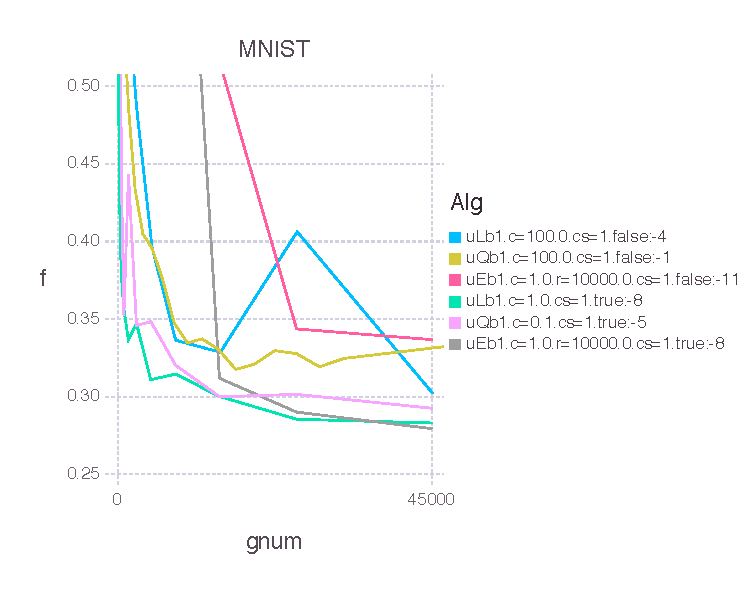
\includegraphics[width= 5in]{Figures/MNISTBLtruefInitialHeuristics.pdf}

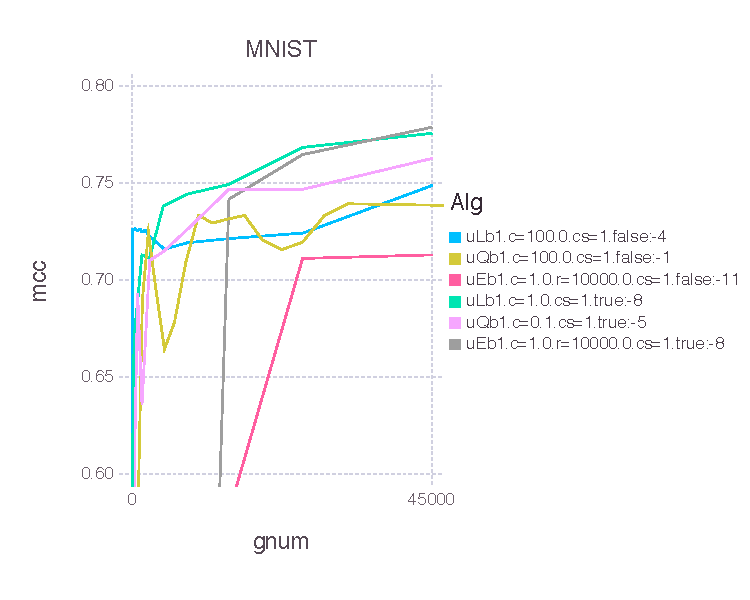
\includegraphics[width= 5in]{Figures/MNISTBLtruemccInitialHeuristics.pdf}

\includegraphics[width= 5in]{Figures/agaricusBLtruefInitialHeuristics.pdf}

\includegraphics[width= 5in]{Figures/agaricusBLtruemccInitialHeuristics.pdf}

\includegraphics[width= 5in]{Figures/SpeechMLtruefInitialHeuristics.pdf}

\includegraphics[width= 5in]{Figures/SpeechMLtruepccInitialHeuristics.pdf}

\includegraphics[width= 5in]{Figures/HIGGSBLtruefInitialHeuristics.pdf}

\includegraphics[width= 5in]{Figures/HIGGSBLtruemccInitialHeuristics.pdf}

\subsection{Adding the variance reduction ($\beta_k=0$ vs other choices)}

\subsection{Different choices for $\beta_k$ sequence}


\subsection{EGR vs SG}

\subsection{Why discard}

     \newpage 
	 
\includegraphics[width= 5in]{Figures/Classify_ConvexBLtruef.pdf} 

\includegraphics[width= 5in]{Figures/Classify_ConvexBLtruepcc.pdf} 

% \includegraphics[width= 3.5in]{Figures/Classify_ConvexBLtruemcc.pdf}


     \newpage 
     
\includegraphics[width= 5in]{Figures/BreakMeBLtruef.pdf} 

\includegraphics[width= 5in]{Figures/BreakMeBLtruepcc.pdf} 

% \includegraphics[width= 3.5in]{Figures/BreakMeBLtruemcc.pdf}

\subsection{Why L2}

On most problems, adding an L2 regularizer did not bring significant improvements to the classification quality of the solution. MNIST showed a slight improvement.

     
\includegraphics[width= 3.5in]{Figures/alphaGoodBLmcc-L2.pdf} 
\includegraphics[width= 3.5in]{Figures/myrandBLmcc-L2.pdf} 

\includegraphics[width= 3.5in]{Figures/SUSYBLmcc-L2.pdf} 
\includegraphics[width= 3.5in]{Figures/MNISTBLmcc-L2.pdf} 

\subsection{EGR vs SG}

All tests were conducted to 1 epoch equivalent limit on sample gradient evaluations

The decimal number growth corresponds to exponential growth in the current batchsize
The \emph{lin} growth corresponds to a linear growth in batchsize

Stepsizes were optimized to give best possible Testing function value within the gradient evaluation limit. 

 \newpage
     
\includegraphics[width= 5in]{Figures/MNISTBLtruef.pdf} 

\includegraphics[width= 5in]{Figures/MNISTBLtruemcc.pdf} 
     
\includegraphics[width= 5in]{Figures/myrandBLtruef.pdf} 

\includegraphics[width= 5in]{Figures/myrandBLtruemcc.pdf} 
     
\includegraphics[width= 5in]{Figures/alphaGoodBLtruef.pdf} 

\includegraphics[width= 5in]{Figures/alphaGoodBLtruemcc.pdf} 
     
\includegraphics[width= 5in]{Figures/SUSYBLtruef.pdf} 

\includegraphics[width= 5in]{Figures/SUSYBLtruemcc.pdf} 

\includegraphics[width= 5in]{Figures/farmSBLtruef.pdf} 

\includegraphics[width= 5in]{Figures/farmSBLtruemcc.pdf} 

\includegraphics[width= 5in]{Figures/SpeechMLfalsef.pdf} 

\includegraphics[width= 5in]{Figures/SpeechMLfalsepcc.pdf} 

\includegraphics[width= 5in]{Figures/HIGGSBLtruef.pdf} 

\includegraphics[width= 5in]{Figures/HIGGSBLtruemcc.pdf} 

\subsection{EGR vs SAG}

Compare total work? Passes?

For SAG, say one pass. What's better? 1/10 of the data, or 1/2 of the data?

Or Schmidt code?

\subsection{DSS vs EGR}

In this section, we show the difference between using the DSS method, and the EGR method with the same exponential growth rate.

\newpage 

\includegraphics[width= 5in]{Figures/MNISTBLtruef-dss.pdf}

\includegraphics[width= 5in]{Figures/MNISTBLtruemcc-dss.pdf}

\includegraphics[width= 5in]{Figures/myrandBLtruef-dss.pdf}

\includegraphics[width= 5in]{Figures/myrandBLtruemcc-dss.pdf}

\includegraphics[width= 5in]{Figures/alphaGoodBLtruef-dss.pdf}

\includegraphics[width= 5in]{Figures/alphaGoodBLtruemcc-dss.pdf}

\includegraphics[width= 5in]{Figures/SUSYBLtruef-dss.pdf}

\includegraphics[width= 5in]{Figures/SUSYBLtruemcc-dss.pdf}

\includegraphics[width= 5in]{Figures/farmSBLtruef-dss.pdf}

\includegraphics[width= 5in]{Figures/farmSBLtruemcc-dss.pdf}

DSS performs so great here, because the small number of datapoints does not warrant the variance reduction at the initial steps. If $\beta$ we small initially, the algorithms might have performed better. 

\subsection{Class - Based memory reduction}

\includegraphics[width= 5in]{Figures/MNISTBLtruefCB.pdf}

\includegraphics[width= 5in]{Figures/MNISTBLtruemccCB.pdf}

\includegraphics[width= 5in]{Figures/myrandBLtruefCB.pdf}

\includegraphics[width= 5in]{Figures/myrandBLtruemccCB.pdf}

\includegraphics[width= 5in]{Figures/agaricusBLtruefCB.pdf}

\includegraphics[width= 5in]{Figures/agaricusBLtruemccCB.pdf}

\includegraphics[width= 5in]{Figures/alphaGoodBLtruefCB.pdf}

\includegraphics[width= 5in]{Figures/alphaGoodBLtruemccCB.pdf}



\newpage
\appendices 
\section{Search for $s_k$ and $u_k$ heuristics}
\label{appendix:heuristics}

Our methods introduce two tunable sequnces, $\{s_k\}$ and $\{u_k\}$. We conduct test to determine whethere a heuristic based on some data properties gives reasonable estimates for the sequences, without the need to fine-tune them. 

\section{Search for $\alpha_k$ heuristics}
\label{appendix:heuristics}



\end{document} 



\subsection{Richard Byrd Argument}

Assume that the join change in error and distance to the solution is modeled by  
\[ 
\begin{pmatrix}
	\beta E[e_k] \\
	x_k-x_\ast 
\end{pmatrix}
= M_k 
\begin{pmatrix}
	\displaystyle \beta e_{k-1} \\
	x_{k-1}-x_\ast 
\end{pmatrix}
\]
where $M_k$ is a scaling matrix.

Appying this relation recursively $k$ times, we arrive at
\[ 
\begin{pmatrix}
	\beta E[e_k] \\
	x_k-x_\ast 
\end{pmatrix}
= 
M_k \cdot M_{k-1} \cdot \ldots \cdot M_1
\begin{pmatrix}
	\displaystyle \beta e_0 \\
	x_0-x_\ast 
\end{pmatrix}
\]

Taking (an induced) norm of both sides, we have that
\[ 
\| 
\begin{pmatrix}
	\beta E[e_k] \\
	x_k-x_\ast 
\end{pmatrix}
\| 
\leq 
\| M_k \|  \cdot \|  M_{k-1} \| \cdot \ldots \cdot \|  M_1 \|
\|
\begin{pmatrix}
	\displaystyle \beta e_0 \\
	x_0-x_\ast 
\end{pmatrix}
\| 
\]

If $\|M_k\| < 1$ for all $k$, then we have that 
\[ 
\lim{k \rightarrow \infty}
\begin{pmatrix}
	\beta E[e_k] \\
	x_k-x_\ast 
\end{pmatrix}
= 
\begin{pmatrix}
	0\\
	0
\end{pmatrix}
\]
 
 
\subsubsection{Richard Approach 1}
 
If we can find a matrix $S$ such that 
\[
\| S M_k S^{-1} \| < 1 
\]
we are done. 
 
\subsubsection{Richard Approach 2}

Assume that there exists a matrix $M$ such that $\|M\| \leq 1$, and
\[
\|M_k x\| \leq \|M x \| 
\]
for all $k$ and $x$, then we have the result that we need. 